%%%%%%%%%%%%%%%%%%%%%%%%%%%%%%%%%%%%%%%%%%%%%%%%%%%%%%%%%%%%%%%%%%%%%%%%%%%%%%%%
%% Plantilla de memoria en LaTeX para la ETSIT - Universidad Rey Juan Carlos
%%
%% Por Gregorio Robles <grex arroba gsyc.urjc.es>
%%     Grupo de Sistemas y Comunicaciones
%%     Escuela Tcnica Superior de Ingenieros de Telecomunicacin
%%     Universidad Rey Juan Carlos
%% (muchas ideas tomadas de Internet, colegas del GSyC, antiguos alumnos...
%%  etc. Muchas gracias a todos)
%%
%% La ltima versin de esta plantilla est siempre disponible en:
%%     https://github.com/gregoriorobles/plantilla-memoria
%%
%% Para obtener PDF, ejecuta en la shell:
%%   make
%% (las imgenes deben ir en PNG o JPG)

%%%%%%%%%%%%%%%%%%%%%%%%%%%%%%%%%%%%%%%%%%%%%%%%%%%%%%%%%%%%%%%%%%%%%%%%%%%%%%%%

\documentclass[a4paper, 12pt]{book}
%\usepackage[T1]{fontenc}
\usepackage{hyperref}
\usepackage[a4paper, left=2.5cm, right=2.5cm, top=3cm, bottom=3cm]{geometry}
\usepackage{times}
\usepackage[latin1]{inputenc}
\usepackage[spanish,activeacute]{babel} % Comenta esta lnea si tu memoria es en ingls
\usepackage{url}
%\usepackage[dvipdfm]{graphicx}
\usepackage{fancybox}
\usepackage{subfigure}
\usepackage{graphicx}
\usepackage{float}  %% H para posicionar figuras
\usepackage[nottoc, notlot, notlof, notindex]{tocbibind} %% Opciones de ndice
\usepackage{latexsym}  %% Logo LaTeX
\usepackage{framed, color}

\title{Memoria del Proyecto}
\author{Adri\'an S\'aez Clemente}

\renewcommand{\baselinestretch}{1.5}  %% Interlineado

\begin{document}

%\renewcommand{\refname}{Bibliografa}  %% Renombrando
\renewcommand{\appendixname}{Ap\'endice}
\definecolor{shadecolor}{rgb}{1,0.8,0.3}
%%%%%%%%%%%%%%%%%%%%%%%%%%%%%%%%%%%%%%%%%%%%%%%%%%%%%%%%%%%%%%%%%%%%%%%%%%%%%%%%
% PORTADA

\begin{titlepage}
\begin{center}
\begin{tabular}[c]{c c}
%\includegraphics[bb=0 0 194 352, scale=0.25]{logo} &

\includegraphics[scale=0.25]{img/logo_vect.png} &
\begin{tabular}[b]{l}
\Huge
\textsf{UNIVERSIDAD} \\
\Huge
\textsf{REY JUAN CARLOS} \\
\end{tabular}
\\
\end{tabular}

\vspace{3cm}


\Large
GRADO EN INGENIER\'IA EN TECNOLOG\'IAS DE LA TELECOMUNICACI\'ON

\vspace{0.4cm}

\large
Curso Acad\'emico 2015/2016

\vspace{0.8cm}

Trabajo Fin de Grado

\vspace{2.5cm}

\LARGE
DESARROLLO Y DESPLIEGUE DE APLICACIONES EN EL \'AMBITO EDUCATIVO

\textit{Dise\~no y despliegue de un planeta de blogs}
\vspace{4cm}

\large
Autor : Adri\'an S\'aez Clemente \\
Tutor : Gregorio Robles Mart\'inez
\end{center}
\end{titlepage}

\newpage
\mbox{}
\thispagestyle{empty} % para que no se numere esta pagina


%%%%%%%%%%%%%%%%%%%%%%%%%%%%%%%%%%%%%%%%%%%%%%%%%%%%%%%%%%%%%%%%%%%%%%%%%%%%%%%%
%%%% Dedicatoria

%\chapter*{}
%\pagenumbering{Roman} % para comenzar la numeracion de paginas en numeros romanos
%\begin{flushright}
%\textit{Dedicado a \\
%mi familia / mi abuelo / mi abuela}
%\end{flushright}

%%%%%%%%%%%%%%%%%%%%%%%%%%%%%%%%%%%%%%%%%%%%%%%%%%%%%%%%%%%%%%%%%%%%%%%%%%%%%%%%
%%%% Agradecimientos

\chapter*{Agradecimientos}
\addcontentsline{toc}{chapter}{Agradecimientos} % si queremos que aparezca en el ndice
\markboth{AGRADECIMIENTOS}{AGRADECIMIENTOS} % encabezado 
Quiero agradecer a mis padres, por haber hecho posible que este largo camino haya dado sus frutos de una manera satisfactoria y exitosa. 
Gracias por vuestro apoyo constante. Sin vosotros, nada de esto pod\'ia haber sucedido.\\

\textit{``El que da, no debe volver a acordarse; pero el que recibe nunca debe olvidar''}\\

%%%%%%%%%%%%%%%%%%%%%%%%%%%%%%%%%%%%%%%%%%%%%%%%%%%%%%%%%%%%%%%%%%%%%%%%%%%%%%%%
%%%% Resumen

\chapter*{Resumen}
\addcontentsline{toc}{chapter}{Resumen} % si queremos que aparezca en el ndice
\markboth{RESUMEN}{RESUMEN} % encabezado
\begin{itemize}
  \item \texttt{Objetivos}: En este proyecto se realiza el desarrollo de una aplicaci\'on web que se basa en la creaci\'on de un planeta de 
  blogs donde sus principales objetivos son la formaci\'on y el aprendizaje de los usuarios.

  \item \texttt{Tecnolog\'ias}: El proyecto ha sido realizado en un entorno Linux, usando \textit{Python} como lenguaje de programaci\'on y Django como 
  framework. Destacar el uso de tecnolog\'ias modernas como \textit{HTML5}, \textit{CSS3}, \textit{AJAX} y dise\~no responsive con \textit{BootStrap} que han dado dinamismo, rapidez, adaptabilidad y 
  est\'etica a la aplicaci\'on.

  \item \texttt{Contexto}: El proyecto est\'a pensado e implementado para un entorno de \'ambito educativo. Concretamente para c\'irculos con un n\'umero variable de 
  usuarios, como aulas de universidad o de instituto, aulas online, cursos en academias, etc.
\end{itemize}


%%%%%%%%%%%%%%%%%%%%%%%%%%%%%%%%%%%%%%%%%%%%%%%%%%%%%%%%%%%%%%%%%%%%%%%%%%%%%%%%
%%%% Resumen en ingls

\chapter*{Summary}
\addcontentsline{toc}{chapter}{Summary} % si queremos que aparezca en el ndice
\markboth{SUMMARY}{SUMMARY} % encabezado
\begin{itemize}
  \item \texttt{Objetives}: This project develops a web application that is based on creating a planet blogs where its main objectives are the formation and learning
  of its members.
  
  \item \texttt{Technologies}: The project was carried out in a Linux environment, using programming language \textit{Python} and \texttt{Django} as framework. Emphasize the use of modern 
  technologies like \textit{HTML5}, \textit{CSS3}, \textit{AJAX} and responsive design (\textit{BootStrap}) given dynamism, speed, adaptability and aesthetics to the application.

  \item \texttt{Context}: The project is designed and implemented for environment education. Specifically for circles with a variable number of users, such as university 
  classrooms or school, online classes, courses in academies, etc.
\end{itemize}


%%%%%%%%%%%%%%%%%%%%%%%%%%%%%%%%%%%%%%%%%%%%%%%%%%%%%%%%%%%%%%%%%%%%%%%%%%%%%%%%
%%%%%%%%%%%%%%%%%%%%%%%%%%%%%%%%%%%%%%%%%%%%%%%%%%%%%%%%%%%%%%%%%%%%%%%%%%%%%%%%
% NDICES %
%%%%%%%%%%%%%%%%%%%%%%%%%%%%%%%%%%%%%%%%%%%%%%%%%%%%%%%%%%%%%%%%%%%%%%%%%%%%%%%%

% Las buenas noticias es que los ndices se generan automticamente.
% Lo nico que tienes que hacer es elegir cules quieren que se generen,
% y comentar/descomentar esa instruccin de LaTeX.

%%%% ndice de contenidos
\tableofcontents 
%%%% ndice de figuras
\cleardoublepage
\phantomsection
\addcontentsline{toc}{chapter}{Lista de figuras} % para que aparezca en el indice de contenidos
\listoffigures % indice de figuras
%%%% ndice de tablas
%\cleardoublepage
%\addcontentsline{toc}{chapter}{Lista de tablas} % para que aparezca en el indice de contenidos
%\listoftables % indice de tablas


%%%%%%%%%%%%%%%%%%%%%%%%%%%%%%%%%%%%%%%%%%%%%%%%%%%%%%%%%%%%%%%%%%%%%%%%%%%%%%%%
%%%%%%%%%%%%%%%%%%%%%%%%%%%%%%%%%%%%%%%%%%%%%%%%%%%%%%%%%%%%%%%%%%%%%%%%%%%%%%%%
% INTRODUCCIN %
%%%%%%%%%%%%%%%%%%%%%%%%%%%%%%%%%%%%%%%%%%%%%%%%%%%%%%%%%%%%%%%%%%%%%%%%%%%%%%%%

\cleardoublepage
\chapter{Introducci\'on}
\label{sec:intro} % etiqueta para poder referenciar luego en el texto con ~\ref{sec:intro}
\pagenumbering{arabic} % para empezar la numeracin de pgina con nmeros

\section{Descripci\'on del proyecto}
\label{sec:descripcion}
En este proyecto se implementa una aplicaci\'on web que consiste en el desarrollo de un planeta de blogs. Est\'a enfocado al \'ambito educativo y puede
ser usado en cualquier entorno que simule un aula, ya sea en universidades, institutos, colegios, academias, cursos online, etc,...

El contenido de la aplicaci\'on recoge autom\'aticamente mensajes o entradas de un conjunto de blogs externos que comparten una tem\'atica com\'un.

El tutor ser\'a el responsable de crear hilos donde los alumnos podr\'an suscribirse y formar parte de la tem\'atica de inter\'es. Dentro de cada hilo,
los alumnos podr\'an visualizar las entradas del conjunto de blogs que est\'an suscritos a ese hilo.

Como novedad incluye la posibilidad de interactuar, valorar y comentar los mensajes de compa\~neros de una forma divertida mediante un proceso de 
gamificaci\'on. En este proceso los participantes de cada hilo podr\'an luchar por un puesto en la clasificaci\'on definitiva consiguiendo 
puntos (llamados planets) y subiendo de nivel seg\'un el compromiso y la capacidad de interacci\'on de cada alumno.

Existe una secci\'on de b\'usqueda para poder encontrar entradas introduciendo nick de usuario y/o identificador de entrada. Y adem\'as, dentro de la
aplicaci\'on se puede encontrar dos secciones con las bases de las puntuaciones y las estad\'isticas generales de cada usuario.

\section{Contexto tecnol\'ogico}
\label{sec:contexto}
Actualmente, la sociedad se encuentra en un proceso de evoluci\'on enorme en la era de la tecnolog\'ia. Esta evoluci\'on llama a la mayor\'ia 
de los usuarios del mundo que usan internet a aprender a manejar nuevas aplicaciones, herramientas o tecnolog\'ias para poder obtener 
conocimientos nuevos y compartirlos.
Todo esto contrasta con un proceso de asimilaci\'on y descubrimiento por otra parte de usuarios con una cierta edad que nunca convivieron con 
el mundo de ``los aparatos e internet''.

En la actualidad tecnol\'ogica, se est\'a produciendo una gran crecimiento y progresi\'on en el \'ambito m\'ovil, con la aparici\'on de los 
denominados smartphones o tel\'efonos inteligentes, aportando una herramienta para conectarse a internet desde cualquier sitio.

El principal problema es la gran diversidad de smartphones y de computadoras modernas, referido tanto a la diversidad hardware 
\rule[1mm]{4mm}{0.1mm}diferentes tama\~nos de pantalla\rule[1mm]{4mm}{0.1mm} como a la variedad de sistemas operativos, e incluso entre ellos, 
diferentes versiones. En este proyecto se ha fijado 
como fuente de test y desarrollo, un sistema operativo Linux Ubuntu 14.04 con un navegador Firefox, que es uno de los navegadores de internet m\'as 
utilizados en la actualidad. El desarrollo de aplicaciones utilizando tecnolog\'ias libres y abiertas, en concreto \textit{CSS}, \textit{HTML} y 
\textit{JavaScript}, tiene como ventaja la creaci\'on de un programa compatible con casi cualquier dispositivo, teniendo que preocuparse exclusivamente 
de peque\~nas variaciones debidas a las diferencias entre navegadores de internet (ya que se cambia
la idea de adaptarse a diferentes sistemas operativos por diferentes navegadores de internet) y a los diferentes tama\~nos de pantalla y m\'etodos
de control (pantallas t\'actiles en m\'oviles y tablets o rat\'on y teclado en ordenadores)







%%%%%%%%%%%%%%%%%%%%%%%%%%%%%%%%%%%%%%%%%%%%%%%%%%%%%%%%%%%%%%%%%%%%%%%%%%%%%%%%
%%%%%%%%%%%%%%%%%%%%%%%%%%%%%%%%%%%%%%%%%%%%%%%%%%%%%%%%%%%%%%%%%%%%%%%%%%%%%%%%
% OBJETIVOS %
%%%%%%%%%%%%%%%%%%%%%%%%%%%%%%%%%%%%%%%%%%%%%%%%%%%%%%%%%%%%%%%%%%%%%%%%%%%%%%%%

\cleardoublepage
\chapter{Objetivos}
\label{chap:objetivos}

\section{Objetivo general}
\label{sec:objetivo-general}
El objetivo principal del proyecto es el desarrollo de una aplicaci\'on educativa que englobe y unifique multitud de temas para que a trav\'es de ellos los usuarios 
puedan interactuar, formarse correctamente y optimizar su aprendizaje.

\section{Objetivos espec\'ificos}
\label{sec:objetivos-especificos}
\begin{itemize}
  \item \textit {Usabilidad sencilla:} Cuanta m\'as sencillez de uso, mayor n\'umero de personas podr\'an manejar la aplicaci\'on. 
  Fue implementada para personas que no est\'an muy familiarizadas con las nuevas tecnolog\'ias, de esta forma se conseguir\'ia 
  abarcar mayor variedad de usuarios.
  \item \textit {Integraci\'on de elementos sociales:} Estamos en un contexto en el que se muestra un gran inter\'es en los elementos sociales. La aplicaci\'on
  integra funciones sociales para la atracci\'on de usuarios. Estas funciones son muy importantes para demostrar la capacidad del usuario 
  de interactuar dentro de un mundo digital. Con un simple comentario, un ``Me gusta'', un ``No me gusta'' o una valoraci\'on por parte del 
  tutor, se crean v\'inculos digitales capaces de mover diferentes sentimientos y pensamientos en las personas como son la curiosidad o el 
  af\'an de superaci\'on.
  \item \textit {Inclusi\'on de gamificaci\'on:} Otro punto importante de la aplicaci\'on es su moneda de cambio, el \textit{planet}. A 
  partir de la creaci\'on de esta moneda se inicia un proceso de gamificaci\'on que alienta la participaci\'on y el compromiso, y mejora la 
  experiencia del usuario. 
  Se obtiene una motivaci\'on y una recompensaci\'on extra con la realizaci\'on de tareas a cambio de estas monedas. As\'i mismo se incita a una 
  mayor colaboraci\'on de los usuarios mediante la retroalimentaci\'on continua sobre el progreso en el ranking. Mejor posici\'on en el ranking 
  significar\'ia el logro de un determinado objetivo personal.\\
  En resumen, volvemos a una de las primeras actividades que realizamos en la vida, jugar. Una actividad que es la principal fuente de 
  aprendizaje cuando somos ni\~nos y el principal motivo de diversi\'on cuando somos adolescentes e, incluso, adultos.
  \item \textit {Adaptabilidad:} La aplicaci\'on ha sido implementada con un dise\~no responsive mediante \textit{BootStrap}. El fin de este dise\~no 
  es mejorar la experiencia del usuario con una adaptabilidad de todos los elementos del contenido de una p\'agina web. Con este fin se logra 
  reducir el uso constante del zoom sobre las webs, de modo que el ancho de pantalla se adapta al dispositivo. Adem\'as se simplifica el 
  acceso a los men\'us y contenidos, y se elimina la ejecuci\'on de aplicaciones secundarias que no funcionan en dispositivos m\'oviles.
  \item \textit {Dinamismo y rapidez:} Otro de los objetivos primordiales es la obtenci\'on de una aplicaci\'on din\'amica. En el momento en que un 
  usuario interactua de alguna manera en cualquier documento \textit{HTML}, tiene la sensaci\'on de que los cambios se producen instant\'aneamente. Esto se ha logrado 
  gracias a la tecnolog\'ia \textit{AJAX}. Esta tecnolog\'ia permite realizar funciones din\'amicas sin necesidad de recargar la p\'agina web, por lo que proporciona 
  m\'as ligereza y velocidad, reduciento el tiempo implicado en cada transacci\'on.
\end{itemize}


%%%%%%%%%%%%%%%%%%%%%%%%%%%%%%%%%%%%%%%%%%%%%%%%%%%%%%%%%%%%%%%%%%%%%%%%%%%%%%%%
%%%%%%%%%%%%%%%%%%%%%%%%%%%%%%%%%%%%%%%%%%%%%%%%%%%%%%%%%%%%%%%%%%%%%%%%%%%%%%%%
% ESTADO DEL ARTE %
%%%%%%%%%%%%%%%%%%%%%%%%%%%%%%%%%%%%%%%%%%%%%%%%%%%%%%%%%%%%%%%%%%%%%%%%%%%%%%%%

\cleardoublepage
\chapter{Tecnolog\'ias utilizadas}

\section{Django y Python} 
\label{sec:djangopython}

\subsection{Django} 
\label{subsec:django}
\texttt{Django} es un framework de desarrollo web de c\'odigo abierto. Est\'a escrito en \textit{Python}, y respeta el paradigma Modelo-Vista-Controlador. 
Este patr\'on se usa para desarrollar software y se basa en la separaci\'on de los datos, de la interfaz del usuario y de la l\'ogica interna. 
En aplicaciones web se usa con mucha frecuencia, d\'onde la vista es la p\'agina HTML, el modelo es el Sistema de Gesti\'on de Base de Datos y la 
l\'ogica interna, y el controlador es el responsable de recibir los eventos y darles soluci\'on.

-Modelo: Es la capa de acceso a la base de datos. Esta capa contiene toda la informaci\'on sobre los datos: como acceder a estos, como validarlos, 
cual es el comportamiento que tiene, y las relaciones entre los datos. Se utiliza como representaci\'on de la informaci\'on en el sistema. Trabaja junto 
a la vista para mostrar la informaci\'on al usuario y es accedido por el controlador para a\~nadir, eliminar, consultar o actualizar datos. 
     
-Vista: Es la capa de la l\'ogica de negocios. Esta capa contiene la l\'ogica que accede al modelo y la delega a la plantilla apropiada. Se presenta 
como un puente entre los modelos y las plantillas.

-Controlador: Es el elemento m\'as abstracto. Recibe, trata y responde los eventos enviados por el usuario o por la propia aplicaci\'on. Interactua 
tanto con el modelo como con la vista.



\subsection{Python} 
\label{subsec:python}
\textit{Python} es un lenguaje de programaci\'on con una sintaxis muy limpia y que favorece un c\'odigo legible. Se ejecuta utilizando un programa intermedio 
llamado int\'erprete, en lugar de compilar el c\'odigo a lenguaje m\'aquina que pueda comprender
y ejecutar directamente una computadora. Tiene una ejecuci\'on m\'as lenta que los lenguajes compilados pero es m\'as flexible y portable.

Tiene la caracter\'istica de tipado din\'amico que se refiere a que no es necesario declarar el tipo de dato que va a contener una determinada 
variable, sino que su tipo se determinar\'a en tiempo de ejecuci\'on seg\'un el tipo del valor al que se asigne, y el tipo de esta variable puede 
cambiar si se le asigna un valor de otro tipo. Adem\'as, \textit{Python} es un lenguaje fuertemente tipado que no permite tratar a una variable como si fuera 
de un tipo distinto al que tiene, es necesario convertir de forma expl\'icita dicha variable al nuevo tipo previamente. 

El int\'erprete de \textit{Python} est\'a disponible en multitud de plataformas (UNIX, Solaris, Linux, DOS, Windows, OS/2, Mac OS, etc.) 
por lo que si no utilizamos librer\'ias espec\'ificas de cada plataforma nuestra aplicaci\'on podr\'a correr en todos estos sistemas sin grandes 
cambios.

Es un lenguaje orientado a objetos. Este concepto se define como un paradigma de programaci\'on en el que los conceptos del mundo real relevantes 
para nuestro problema se trasladan a clases y objetos en nuestra aplicaci\'on. La ejecuci\'on de la aplicaci\'on consiste en una serie de interacciones 
entre los objetos.

En este proyecto, \textit{Python} se usa principalmente para el desarrollo de las vistas en el lado del servidor, donde mediante 
peticiones de los usuarios, recoge y procesa la informaci\'on y devuelve los datos a la presentaci\'on correspondiente. Tambi\'en se usa para recoger el 
modelo de datos y las URLs necesarias para enlazar con las vistas.


\section{HTML5}
\label{sec:html5}
\textit{HTML5} (HyperText Markup Language) Es la versi\'on 5 del lenguaje en el que se escriben las p\'aginas webs. Un lenguaje que s\'olo son capaces 
de leer los \'ultimos navegadores, ya que los que son m\'as anticuados hay algunas etiquetas que no son capaces de interpretar. Sirve para integrar 
contenidos multimedia, flash y para dar un sentido sem\'antico a cada parte de la p\'agina web.

\textit{HTML5} disminuye el tiempo de carga de las p\'aginas y tambi\'en ayuda a bajar el ratio de texto/\textit{HTML} ya que es un lenguaje m\'as simple.
Es un lenguaje m\'as sem\'antico que dota de un significado a las diferentes partes de la p\'agina Web. Ayuda a los buscadores a entender la p\'agina 
web y tambi\'en sirve para que los navegadores muestren de forma inteligente diferentes versiones de la p\'agina Web sin tener que usar plug-ins para 
dispositivos espec\'ificos.

\textit{HTML5} incluye m\'as elementos gr\'aficos y multimedia. Permite la inserci\'on de etiquetas canvas, que sustituyen a las animaciones en Flash y tambi\'en 
permite incluir de forma muy sencilla v\'ideos, m\'usica y otros elementos multimedia como por ejemplo los videojuegos. Adem\'as incluye la 
geolocalizaci\'on. Es posible saber desde que lugar se esta visualizando un sitio Web, gracias a sistemas de referenciaci\'on como el GPS, 
la tecnolog\'ia 3G de los dispositivos m\'oviles o las conexiones tipo WiFi.

\textit{HTML5} permite el uso de las Webs offline. Aunque no tengas conexi\'on a Internet si el programador lo desea podr\'as ver parte o toda la p\'agina Web, 
e incluso interactuar con los contenidos. Esto mejora la usabilidad de la Web y permite al usuario trabajar con aplicaciones online desconectado, 
algo importante en los dispositivos m\'oviles cuando te mueves en entornos en los que no tienes una conexi\'on de calidad.


\section{JavaScript}
\label{sec:javascript}


\subsection{jQuery}
\label{subsec:jquery}
\textit{jQuery} es una librer\'ia \textit{JavaScript} pensada y creada para acceder f\'acilmente a los elementos del DOM, para automatizar tareas comunes 
y simplificar las labores complicadas de \textit{JavaScript}.

Esta librer\'ia da una serie de ventajas: 
\begin{itemize}
  \item Facilidad de acceso en el documento.
  \item Para la localizaci\'on de partes espec\'ificas en la estructura del documento \textit{HTML}, \textit{jQuery} tiene un mecanismo de selector s\'olido y 
eficiente con el que puede recuperar piezas exactas del DOM (Document Object Model).
  \item Modifica la apariencia de un sitio web. Puede llenar vacios que \textit{CSS} no puede cubrir. Y tambi\'en puede cambiar clases y estilos aplicados 
en \textit{CSS} incluso despu\'es de que la p\'agina ya est\'e renderizada en el navegador.
  \item Altera contenidos del documento. \textit{jQuery} puede modificar cualquier contenido en el documento.
  \item Responde a la interacci\'on del usuario. Ofrece una forma elegante de controlar acciones y nos presenta una amplia variedad de eventos 
que responden a diversas acciones del usuario sin necesidad de saturar el c\'odigo \textit{HTML}.
  \item Simplifica tareas comunes de \textit{JavaScript}. Esta librer\'ia ofrece mejoras en el momento de desarrollar en \textit{JavaScript}, nos ahorra tiempo 
y el c\'odigo ser\'a siempre m\'as limpio y sencillo.
\end{itemize}


\subsection{jQuery-ui}
\label{subsec:jqueryui}
\textit{jQuery-ui} es una biblioteca de componentes para la librer\'ia \textit{jQuery} que le a\~naden un conjunto de plug-ins (drag, drop, sorting, 
resizing, etc.), widgets (accordion, date picker, dialog, slider y tabs) y efectos visuales (show, hide, toggle, color animation, class manipulation, etc.)
para la creaci\'on de aplicaciones web.

El ``accordion'' es el widget que se usa en la pesta\~na de estad\'isticas y sirve para mostrar la informaci\'on detallada de un solo usuario. Si clicas en 
otro nombre del acorde\'on, se oculta el usuario seleccionado anteriormente y se expande la informaci\'on del usuario actual.

\subsection{AJAX}
\label{subsec:ajax}
\textit{AJAX} (Asynchronous \textit{JavaScript} And \textit{XML}) se usa para la transferencia de informaci\'on mediante \textit{JavaScript}. Esta informaci\'on fluye por dos canales 
entre el cliente y el servidor, y puede ser transferida en formato \textit{XML}, texto simple u otros est\'andares como JSON.

\textit{AJAX} sirve para actualizar una porci\'on de nuestra p\'agina web sin necesidad de cargar el c\'odigo, atributos gr\'aficos e im\'agenes de nuevo. Esto
provoca mayor rapidez en la interacci\'on cliente-servidor. El cliente no percibe demoras puesto que las comunicaciones se producen en segundo plano y
no hay interrupciones. \textit{AJAX} tiene la capacidad de comprimir las funciones de una aplicaci\'on en un espacio \textit{HTML} m\'as reducido de lo que antes pod\'ia
ser necesario.

Algunos de los inconvenientes de \textit{AJAX} son el aumento de la complejidad en el desarrollo de aplicaciones, problemas con restricciones de seguridad 
relacionados con su uso, y aumento de la dificultad en la indexaci\'on para los motores de b\'usqueda ya que el contenido deja de ser est\'atico.\\

Dentro de la aplicaci\'on, la mayor\'ia de las acciones que ocurren sin recargar la p\'agina se produce por el intercambio de datos entre cliente y servidor 
mediante \textit{AJAX}, con peticiones \texttt{GET} y \texttt{POST}. Como por ejemplo, agregar una asignatura a ``Mis hilos'', enviar y eliminar un 
comentario, o clicar en los botones de ``Me gusta/No me gusta''.


\subsection{JSON}
\label{subsec:json}
JSON es un formato de fichero de texto ligero utilizado para el intercambios de datos. B\'asicamente JSON describe los datos con una sintaxis dedicada 
que se usa para identificar y gestionar los datos. Este formato es simple, directo, ligero y muy importante para el desarrollo de aplicaciones basadas 
en lenguajes Web y para dispositivos m\'oviles. Cada dato es un par nombre/valor.

En las vistas del proyecto, JSON es un formato que se usa para enviar datos de determinados modelos a la p\'agina \textit{HTML}. Las funciones del fichero 
\textit{JavaScript} captan los modelos en este formato para despu\'es recopilar dicha informaci\'on y manejarla seg\'un la l\'ogica de cada funci\'on. Por 
ejemplo, para poder mostrar un popup con la informaci\'on de un usuario al pasar el rat\'on por encima de su nombre, la funci\'on \textit{JavaScript} 
recolect\'o el modelo de datos \texttt{User} para poder elegir la informaci\'on del usuario de inter\'es y manejarla de tal forma que en la p\'agina se 
contemple un popup con dicha informaci\'on.

\section{CSS3}
\label{sec:css3}
\textit{CSS} (Cascading Style Sheets) se refiere a la tecnolog\'ia desarrollada para separar la presentaci\'on de la estructura \textit{HTML} de un sitio web. 
Esta tecnolog\'ia aplica reglas de estilo a los elementos \textit{HTML}, quedando de esta manera separada de la estructura \textit{HTML}. Poco a poco este lenguaje se 
ha ido haciendo m\'as importante entre los dise\~nadores gracias a toda la facilidad de uso, y los resultados que son muy flexibles.

\textit{CSS3} es la versi\'on 3 de \textit{CSS}, donde se definen las caracter\'isticas de este lenguaje, a\~nadiendo muchas funciones y mejorado otras.
En una hoja de estilo \'o fichero .css, se definen reglas en las cuales se van a aplicar diferentes y muy variados efectos a las etiquetas \textit{HTML}.
Las reglas se forman a partir de selectores, atributos y valores. 

Los selectores se usan para definir sobre qu\'e etiqueta \textit{HTML} vamos a aplicar atributos y valores. Existen selectores de etiquetas \textit{HTML}, los cuales 
se utilizan escribiendo el nombre de la etiqueta a la que se aplicar\'a el estilo. Tambi\'en existen selectores de identificador, que son aquellos que 
empiezan por ``\#'' seguido del id de la etiqueta a la que queremos darle los atributos. Y por \'ultimo, selectores de clase que se escriben en el 
documento \textit{CSS} comenzando por ``.'' y va seguido del nombre de la clase de la etiqueta.

Los atributos son efectos o estilos que aplicaremos a las etiquetas \textit{HTML}. Una vez definidos los selectores y los atributos, se les da un valor a 
los atributos. Se aplican sobre texto, enlaces, im\'agenes, listas, tablas, formularios, etc. Tambi\'en incluye la posibilidad de realizar animaciones con 
porcentajes de tiempo.

En el proyecto, cada documento \textit{HTML} lleva consigo su fichero \textit{CSS}. Gracias a \'el, cada p\'agina muestra los colores apropiados, los distintos
tipos de bordes para los diferentes elementos o los distintos tipos de letras con sus efectos en cursiva, negrita, etc.

Con el uso de \textit{CSS3}, lo m\'as destacado son algunas de las animaciones que se encuentran por toda la aplicaci\'on. Por ejemplo, en la p\'agina de 
registro, mientras el usuario est\'a escribiendo su nick de usuario en el formulario, justo debajo aparece una rueda giratoria y cuando deja de escribir 
ense\~na una l\'inea informativa que aclara si es ``nick correcto'' o ``nick ocupado''.


\section{BootStrap}
\label{sec:bootstrap}
\textit{BootStrap} es un framework originalmente creado por Twitter, que permite crear interfaces web con \textit{CSS} y \textit{JavaScript} y cuya 
particularidad es la de adaptar la interfaz del sitio web al tama\~no del dispositivo en que se visualice, ya sea pantalla de PC, port\'atil, tablet, 
Smartphone,.. Esta t\'ecnica de dise\~no y desarrollo se conoce como dise\~no adaptativo o `responsive design'.

El beneficio de usar dise\'no adaptativo en un sitio web, es principalmente que el sitio web se adapta autom\'aticamente al dispositivo desde donde 
se acceda. Aun ofreciendo todas las posibilidades que ofrece \textit{BootStrap} a la hora de crear interfaces web, los dise\'nos creados con \textit{BootStrap} son 
simples, limpios e intuitivos, esto les da agilidad a la hora de cargar y adaptarse a otros dispositivos. El framework trae varios elementos con 
estilos predefinidos f\'aciles de configurar como botones, men\'us desplegables, formularios incluyendo todos sus elementos, y \textit{jQuery} integrado para 
ofrecer ventanas y tooltips din\'amicos.

El uso de \textit{BootStrap} ofrece una serie de ventajas:
\begin{itemize}
  \item Permite tener un mismo lenguaje para la comunicaci\'on entre dise\~nadores y equipo de desarrollo.
  \item Tiene un comportamiento unificado entre diferentes navegadores.
  \item Es compatible con navegadores modernos, dispositivos y navegadores antiguos (hasta Internet Explorer 8)
  \item Soporte avanzado para Responsive web Design (se podr\'ia utilizar como NO responsive pero forz\'andolo).
  \item Comportamiento y plugins basados en \textit{jQuery} muy \'utiles y usados habitualmente.
  \item \textit{BootStrap} es responsive y viene con un grid de 12 columnas y cuenta con diferentes `Media queries': 768 px (tablets), 992 px (Desktop) y 
  1200 px (Large Desktop) + Mobile (por defecto en \textit{BootStrap}).
  \item Y por \'ultimo y m\'as importante, usa un sistema de rejillas.
\end{itemize}

\textit{BootStrap} incluye una rejilla flu\'ida pensada para m\'oviles. Esta rejilla crece hasta 12 columnas a medida que crece el tama\~no de la pantalla del 
dispositivo. \textit{BootStrap} incluye clases \textit{CSS} para utilizar la rejilla directamente en tus dise\~nos y tambi\'en define mixins de LESS para que puedas 
crear dise\~nos m\'as sem\'anticos.

\begin{figure}[htbp] 
  \label{figura:bootstrap}
  \centering
  \shadowbox{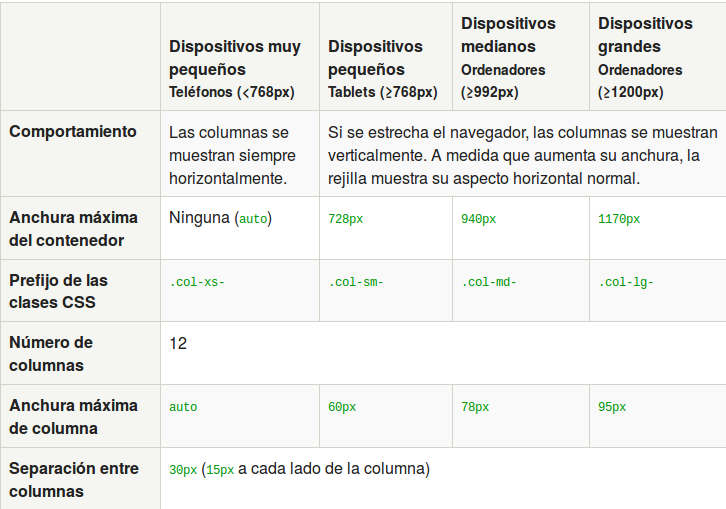
\includegraphics[width=17cm, keepaspectratio]{img/BootStrap}}
  \caption{Tama\~nos en diferentes dispositivos}
\end{figure}

El dise\~no de p\'aginas basado en rejilla se realiza mediante filas y columnas donde se colocan los contenidos. La rejilla de \textit{BootStrap} funciona del
siguiente modo: Las filas siempre se definen dentro de un contenedor de clase .container (anchura fija) o de tipo .container-fluid (anchura variable), 
de esta forma las filas se alinean bien y muestran el padding correcto. Las filas se utilizan para agrupar horizontalmente a varias columnas. 
El contenido siempre se coloca dentro de las columnas, ya que las filas s\'olo deber\'ian contener como hijos elementos de tipo columna. \textit{BootStrap} 
define muchas clases \textit{CSS} (como por ejemplo .row y .col-xs-4) para crear rejillas r\'apidamente. La separaci\'on entre columnas se realiza aplicando 
padding. Para contrarrestar sus efectos en la primera y \'ultima columnas, las filas (elementos .row) aplican m\'argenes negativos. Las columnas de la 
rejilla definen su anchura especificando cu\'antas de las 12 columnas de la fila ocupan. Si por ejemplo quieres dividir una fila en tres columnas 
iguales, utilizar\'ias la clase .col-xs-4 (el 4 indica que cada columna ocupa 4 de las 12 columnas en las que se divide cada fila).

\begin{figure}[htbp] 
  \label{figura:bootstrap1}
  \centering
  \subfigure[Dispositivo mediano]{\shadowbox{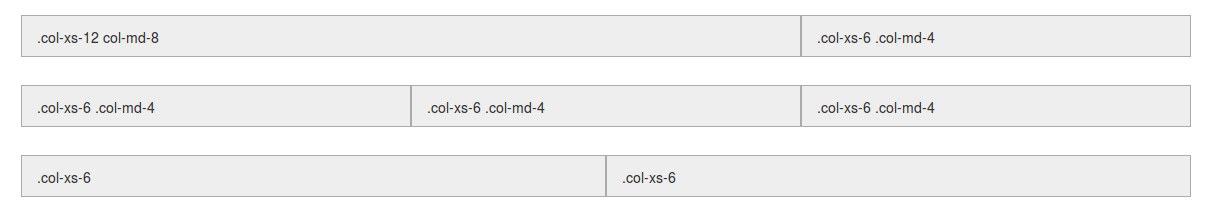
\includegraphics[width=11cm]{img/BootStrapMD}}}
  \subfigure[Dispositivo peque\~no]{\shadowbox{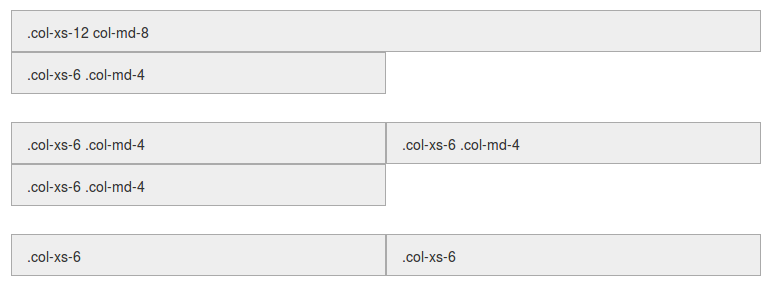
\includegraphics[width=11cm]{img/BootStrapXS}}}
  \caption{Ejemplo para dispositivos medianos (clase col-md-x) y peque\~nos (clase col-xs-x)}
\end{figure}

Por \'ultimo, hay que decir que \textit{BootStrap} permite el anidamiento, el reordenamiento y el desplazamiento de las columnas 
(tanto por la izquierda como por la derecha).

En la aplicaci\'on se usa un plugin de ventanas modales de \textit{BootStrap} que cabe mencionar. El plugin se llama \textit{BootStrapDialog} y es una 
ventana de cuadro de di\'alogo / emergente 
que aparece en la parte superior de la p\'agina actual. Esta ventana es un cuadro de di\'alogo con cabecera, cuerpo y footer, y adem\'as tiene a\~nadidos 
botones para realizar la acci\'on que se desee. 

En la p\'agina principal de un hilo en la parte del tutor, puede saltar dicha ventana si el tutor intenta 
eliminar una entrada o un alumno suscrito.


\section{Git}
\label{sec:git}
\textit{Git} es un sistema de control de versiones distribuido de c\'odigo abierto relativamente nuevo que nos ofrece las mejores caracter\'isticas en la 
actualidad, pero sin perder la sencillez. Es el sistema de control de versiones m\'as usado por desarrolladores en el mundo. 
A los programadores ayuda a ser m\'as eficientes en su trabajo, ya que ha universalizado las herramientas de control de versiones del software que 
hasta entonces no estaban tan popularizadas y tan al alcance del com\'un de los desarrolladores.

\textit{Git} es multiplataforma, por lo que puedes usarlo y crear repositorios locales en todos los sistemas operativos m\'as comunes, Windows, Linux o Mac. 
Existen multitud de GUIs (Graphical User Interface o Interfaz de Usuario Gr\'afica) para trabajar con \textit{Git}. Una de ellas es por l\'inea de comandos.

Dentro de este proyecto, para hacer uso de este sistema de control de versiones se ha utilizado \textit{GitHub}. \textit{GitHub} es un servicio para alojamiento de 
repositorios de software gestionados por el sistema de control de versiones \textit{Git}. Por tanto, \textit{Git} es algo m\'as general que nos sirve para controlar 
el estado de un desarrollo a lo largo del tiempo, mientras que \textit{GitHub} es un sitio web que usa \textit{Git} para ofrecer a la comunidad de desarrolladores 
repositorios de software. En definitiva, \textit{GitHub} es un sitio web pensado para hacer posible el compartir el c\'odigo de una manera m\'as f\'acil.

Una de sus caracter\'isticas m\'as importantes es la posibilidad de crear ramificaciones y trabajar en cada una de ellas sin afectar al resto, permitiendo 
estar trabajando con varios aspectos complejos de un programa de forma simult\'anea y completamente aislada, o dando la posibilidad de dividir un proyecto 
para desarrollar partes espec\'ificas para un determinado servicio o un determinado cliente, e incluso facilitar el desarrollo de proyectos en los que 
trabajen varias personas.

\section{Pivotal tracker}
\label{sec:pivotal}
Pivotal Tracker es un servicio para la gesti\'on \'agil de proyectos y colaboraci\'on creado por Pivotal Labs. Esta herramienta incluye soporte 
para el intercambio de archivos y gesti\'on de tareas, as\'i como para la planificaci\'on de las iteraciones. Adem\'as posee una API para extensiones y 
herramientas de terceros.

Las ventajas de usar Pivotal Tracker son:
\begin{itemize}
  \item Es gratis y no tiene ning\'un tipo de limitaci\'on. Es decir no hay licencia ``community'' y otra ``enterprise'', ni nada parecido.
  \item Esta en la nube. Con lo que no tenemos que instalar nada en nuestros ordenadores, todo lo haremos a trav\'es del navegador.
  \item Se centra en algo muy interesante que es la gesti\'on de la pila de producto, y m\'etricas como la velocidad.
  \item Se puede usar para trabajo con equipos descentralizados, puesto que est\'a en internet. Adem\'as se puede crear varios perfiles de acceso por 
  lo que podr\'ia haber usuarios que, por ejemplo, s\'olo tienen permiso para ver las cosas, pero no para modificarlas.
  \item Guarda hist\'orico de nuestras acciones.
\end{itemize}

Al logarse en la p\'agina web se muestra un ``Dashboard'' que es el panel de control donde se incluyen todos los proyectos creados.

Al crearse un nuevo proyecto, todas las historias de usuario se ordenan en varias pilas que podemos ver en la zona principal del proyecto.
\begin{itemize}
  \item {\bfseries Current}: Son las historias de usuario que tenemos planificadas para el sprint en el que estamos.
  \item {\bfseries Backlog}: Son las historias de usuario que tenemos planificadas para sprints futuros. Pivotal Tracker nos va marcando 
  donde empiezan los sprints. Esto lo hace de forma autom\'atica en funci\'on de nuestra velocidad media.
  \item {\bfseries Icebox}: Son historias de usuario que todav\'ia no tenemos planificadas.
  \item {\bfseries Done}: Esta pila por defecto no se muestra, pero si la activamos nos ense\~nar\'ia los sprint que ya han pasado. Aqu\'i podemos ver cu\'ando se 
  hizo qu\'e. 
\end{itemize}

\section{Crontab}
\label{sec:crontab}
\textit{Crontab} es una herramienta especializada en la automatizaci\'on de tareas y su principal pilar es el cron. 
En el sistema operativo Unix, cron es un administrador regular de procesos en segundo plano (demonio) que ejecuta procesos o guiones a intervalos 
regulares (por ejemplo, cada minuto, d\'ia, semana o mes). Los procesos que deben ejecutarse y la hora en la que deben hacerlo se especifican en el fichero 
\textit{Crontab}.
El demonio cron inicia de \texttt{/etc/rc.d/} o \texttt{/etc/init.d} dependiendo de la distribuci\'on. Cron se ejecuta en el background, revisa cada minuto la tabla de tareas
\textit{Crontab} \texttt{/etc/crontab} o en \texttt{/var/spool/cron} en b\'usqueda de tareas que se deban cumplir. Como usuario podemos agregar comandos o scripts con tareas a cron 
para automatizar algunos procesos. Esto es \'util por ejemplo para automatizar la actualizaci\'on de un sistema, ejecutar un script que tenemos para 
contabilizar cualquier asunto o bien para avisarnos peri\'odicamente del estado de alg\'un servicio en nuestro servidor Linux.
Para automatizar una tarea necesitamos un script hechos por nosotros, el cual queremos ejecutar. En este caso bastar\'a con escribir nuestro script y 
luego darle permisos de ejecuci\'on: 
  \begin{verbatim} #chmod +x miscript.py \end{verbatim}
Para a\~nadir el cron, ejecutamos la edici\'on del \textit{Crontab} con \begin{verbatim} crontab -e \end{verbatim} en algunas distros (como debian) nos da la opcion 
de elegir el editor de textos que deseemos, los dem\'as nos quedamos con \textit{vi}. El archivo \textit{Crontab} lucir\'a algo as\'i: 
  \begin{verbatim} # m h dom mon dow user command \end{verbatim} donde:
\begin{itemize}
  \item {\bfseries m}: Corresponde al minuto en que se va a ejecutar el script, el valor va de 0 a 59.
  \item {\bfseries h}: La hora exacta, se maneja el formato de 24 horas, los valores van de 0 a 23, siendo 0 las 12:00 de la medianoche.
  \item {\bfseries dom}: Hace referencia al d\'ia del mes. Por ejemplo, se puede especificar 15 si se quiere ejecutar cada d\'ia 15.
  \item {\bfseries mon}: Hace referencia al mes. Por ejemplo, se puede especificar 11 si se quiere ejecutar cada mes de noviembre.
  \item {\bfseries dow}: Significa el d\'ia de la semana, puede ser num\'erico (0 a 7, donde 0 y 7 son domingo) o las 3 primeras letras del d\'ia en 
  ingl\'es: mon, tue, wed, thu, fri, sat, sun.
  \item {\bfseries user}: Define el usuario que va a ejecutar el comando, puede ser root, u otro usuario diferente siempre y cuando tenga permisos de 
  ejecuci\'on del script.
  \item {\bfseries command}: Refiere al comando o a la ruta absoluta del script a ejecutar. Por ejemplo: /home/usuario/scripts/actualizar.sh. Si acaso 
  llama a un script, \'este debe ser ejecutable.
\end{itemize}
Dentro del c\'odigo de la aplicaci\'on, existe un script llamado \texttt{actualizar.py}. Es el encargado de guardar las entradas autom\'aticamente en base
de datos. Para su automatizaci\'on se cre\'o un cron que lo ejecuta cada minuto. Para ello, el fichero \textit{Crontab} fue modificado a\~nadiendo las dos \'ultimas 
l\'ineas: 
{\footnotesize\begin{verbatim} 
      # Edit this file to introduce tasks to be run by cron.
      # 
      # Each task to run has to be defined through a single line
      # indicating with different fields when the task will be run
      # and what command to run for the task
      # 
      # To define the time you can provide concrete values for
      # minute (m), hour (h), day of month (dom), month (mon),
      # and day of week (dow) or use '*' in these fields (for 'any').# 
      # Notice that tasks will be started based on the cron's system
      # daemon's notion of time and timezones.
      # 
      # Output of the crontab jobs (including errors) is sent through
      # email to the user the crontab file belongs to (unless redirected).
      # 
      # For example, you can run a backup of all your user accounts
      # at 5 a.m every week with:
      # 0 5 * * 1 tar -zcf /var/backups/home.tgz /home/
      # 
      # For more information see the manual pages of crontab(5) and cron(8)
      # 
      # m h  dom mon dow   command
      
      */1 * * * * cd /home/nombreMaquina/directorioGitProyecto/PlanetaBlogs/TFG;
      python actualizar.py; 
\end{verbatim}}

%%%%%%%%%%%%%%%%%%%%%%%%%%%%%%%%%%%%%%%%%%%%%%%%%%%%%%%%%%%%%%%%%%%%%%%%%%%%%%%%
%%%%%%%%%%%%%%%%%%%%%%%%%%%%%%%%%%%%%%%%%%%%%%%%%%%%%%%%%%%%%%%%%%%%%%%%%%%%%%%%
% DISEO E IMPLEMENTACIN %
%%%%%%%%%%%%%%%%%%%%%%%%%%%%%%%%%%%%%%%%%%%%%%%%%%%%%%%%%%%%%%%%%%%%%%%%%%%%%%%%

\cleardoublepage
\chapter{Dise\~no e implementaci\'on}

\section{Arquitectura general} 
\label{sec:arquitectura}
En esta secci\'on se define la estructura interna del proyecto. En la figura~\ref{fig:arquitectura} se muestra una imagen detallada de los directorios y 
subdirectorios con sus respectivos archivos que hacen posible el funcionamiento de la aplicaci\'on.
En dicha estructura cabe destacar los siguientes bloques:
\begin{itemize}
  \item {\bfseries actualizar.py}: Es un script \textit{Python} que realiza la funci\'on de actualizaci\'on autom\'atica de entradas. Cada vez que un alumno ingresa
  una nueva entrada en su blog, este script es el encargado de detectar esos nuevos cambios a trav\'es de los RSS guardados en base de datos. Se ejecutar\'a
  cada minuto.
  \item {\bfseries bbdd.sqlite}: Es la base de datos del proyecto donde se van a guardar todos los datos estructurados a partir de los modelos definidos en 
  \texttt{models.py}
  \item {\bfseries planetablogs}: Contiene la parte fundamental de la funcionalidad del proyecto. Dentro de este directorio se encuentran distintos ficheros
  python. \texttt{admin.py} hace la funci\'on de modificar la interfaz de administraci\'on que \texttt{Django} genera por defecto. En \texttt{formularios.py}
  se definen todos los formularios que ser\'an utilizados por los usuarios dentro de la aplicaci\'on para crear nuevos elementos o actualizar elementos
  existentes en la base de datos. En \texttt{models.py} se encuentran los modelos que se convertir\'an en tablas dentro de la base de datos. Estos modelos se
  encargan de representar los datos dentro de la aplicaci\'on y contienen los campos necesarios y el comportamiento de los datos que ser\'an almacenados.
  Por \'ultimo, \texttt{views.py} es un fichero donde se implementa toda la l\'ogica del proyecto llevando a cabo todas las peticiones de los usuarios.
  \item {\bfseries plantillas}: En este directorio se encuentran todas las plantillas de los documentos \textit{HTML} que ser\'an enviados al usuario y 
  mostrados por el navegador para dar una interfaz gr\'afica a la aplicaci\'on.
  \item {\bfseries static}: Esta carpeta contiene las librer\'ias \textit{BootStrap}, \textit{jQuery} y \textit{jQuery-ui}. Tambi\'en incluye un subdirectorio
  donde se guardan tanto las im\'agenes propias del proyecto como las im\'agenes de perfil introducidas por los usuarios en el campo de registro. 
  Y adem\'as, se localizan todos los ficheros \textit{.js} y \textit{.css} que a\~nadir\'an funcionalidad y definir\'an el dise\~no a su respectivo 
  documento \textit{HTML} o p\'agina web.
  \item {\bfseries TFG}: Contiene ficheros b\'asicos para el correcto funcionamiento de la aplicaci\'on.\\ \texttt{settings.py} es un fichero de 
  configuraci\'on que contiene todas las rutas relativas o directorios necesarios. \texttt{urls.py} define todas las URLs y las asocia a una vista en
  \texttt{views.py} que se encargar\'a de procesar las peticiones de los clientes.\\\\\\\\\\\\\\\\\\\\\\\\\\\\
\end{itemize}


\begin{figure}
  \centering
  \shadowbox{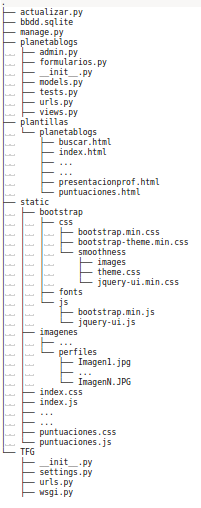
\includegraphics[width=9cm, keepaspectratio]{img/tree}}
  \caption{Estructura de directorios. Utilizando la herramienta \href{http://www.computerhope.com/unix/tree.htm}{\textit{tree}}.}
  \label{fig:arquitectura}
\end{figure}


\section{Estructura Django del proyecto} 
\label{sec:estructuradjango}
En esta secci\'on se expone una descripci\'on m\'as detallada del funcionamiento del proyecto. Se empieza con una introducci\'on que cuenta la estructura
o esqueleto del sistema \texttt{Django} y termina con una explicaci\'on m\'as espec\'ifica del dise\~no de las distintas partes implementadas en \'el.


\subsection{Introducci\'on a la estructura de Django} 
\label{sec:introestructura}
En la figura~\ref{fig:introestructura} se muestra un boceto de c\'omo funciona \texttt{Django} internamente. Hay dos partes diferenciadas que separan al
cliente del servidor. El cliente es el navegador y el servidor \texttt{Django}. El cliente tiene las funciones de enviar peticiones al servidor y de 
mostrar la presentaci\'on o interfaz al usuario final. Las peticiones las lleva a cabo el cliente a trav\'es del usuario en el momento en que \'este 
pulsa sobre un enlace o pide una URL en concreto en la barra del navegador mientras que el servidor se encarga de procesar dichas peticiones y de 
transferir los datos necesarios al cliente para que puedan ser visualizados por el usuario.

El proceso del sistema \texttt{Django} comienza con una solicitud por parte del usuario. Esta solicitud puede ser de tipo \texttt{GET} para conseguir 
informaci\'on de la base de datos o de tipo \texttt{POST} para guardar o modificar informaci\'on de la base de datos. La petici\'on es enviada por el 
cliente o navegador mediante una URL. \texttt{Django} atrapar\'a esa URL y comprobar\'a en su fichero \texttt{urls.py} si la URL existe o no 
\rule[1mm]{4mm}{0.1mm}en el caso de que la URL no exista \texttt{Django} devolver\'a al cliente una plantilla \textit{HTML} de error\rule[1mm]{4mm}{0.1mm}.
En caso de que la petici\'on sea correcta, \texttt{Django} mediante el \textit{URLConf} interpretar\'a dicha URL y se dirigir\'a a la vista apropiada 
\rule[1mm]{4mm}{0.1mm}en el fichero \texttt{urls.py} cada URL est\'a asociada a una vista\rule[1mm]{4mm}{0.1mm}. Dentro del fichero \texttt{views.py} se
ubicar\'a la vista que se necesita, la cual se encargar\'a de interactuar con el modelo, bien para obtener datos \rule[1mm]{4mm}{0.1mm}en caso de 
petici\'on \texttt{GET}\rule[1mm]{4mm}{0.1mm} o bien para guardar o modificar alg\'un elemento del modelo de datos \rule[1mm]{4mm}{0.1mm}en caso de 
petici\'on \texttt{POST}\rule[1mm]{4mm}{0.1mm}. La vista se redirigir\'a al fichero \texttt{forms.py} en caso de que la petici\'on se hubiera dado a trav\'es
de un formulario. Por \'ultimo, la funci\'on final de la vista ser\'a la de llamar a la plantilla situada en el directorio de templates, y \'esta plantilla
se ocupar\'a de renderizar la respuesta a la solicitud del cliente.

\texttt{Django} se responsabiliza del env\'io de los diferentes documentos que se encuentran en la parte del servidor. La respuesta al cliente se traduce
en forma de documento \textit{HTML}. Este documento contendr\'a las plantillas necesarias para mostrar los datos servidos al cliente por parte de 
\texttt{Django}. El servidor tambi\'en se encarga de servir los ficheros referenciados dentro de ese documento \textit{HTML}. El fichero \textit{JavaScript}
a\~nadir\'a la funcionalidad necesaria \rule[1mm]{4mm}{0.1mm}mediante \textit{JavaScript} puro, \textit{jQuery} o \textit{jQuery-ui}\rule[1mm]{4mm}{0.1mm}
para dar distintos comportamientos a los datos servidos \rule[1mm]{4mm}{0.1mm}datos proporcionados directamente en plantillas o serializados con formato
\textit{JSON}\rule[1mm]{4mm}{0.1mm}

En la interacci\'on del usuario con la interfaz recibida por el cliente cabe destacar el uso de \textit{AJAX}. El usuario usar\'a la aplicaci\'on de tal
modo que cuando env\'ie una petici\'on \textit{AJAX} a trav\'es del fichero \textit{JavaScript} referenciado en la p\'agina \textit{HTML} que est\'e manejando,
el servidor contestar\'a enviando los datos que pide sin necesidad de recargar esa p\'agina desde la cual se realiz\'o dicha petici\'on \textit{AJAX}.
\begin{figure}
  \centering
  \shadowbox{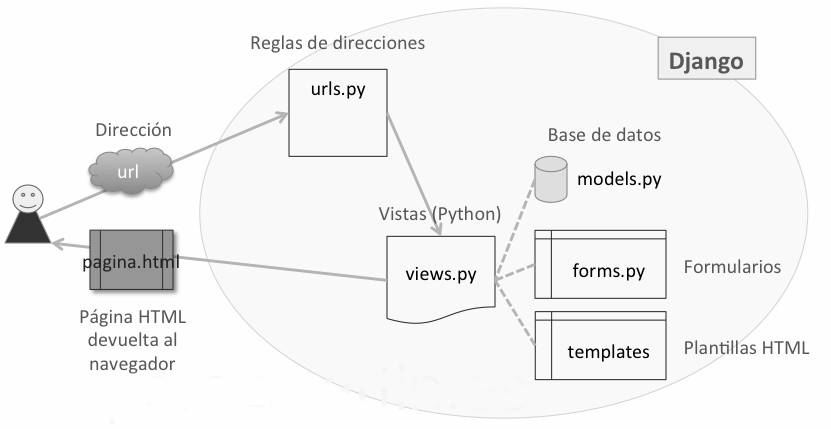
\includegraphics[width=17cm, keepaspectratio]{img/diagrama}}
  \caption{\textit{Estructura general del sistema \texttt{Django}.}}
  \label{fig:introestructura}
\end{figure}


\subsection{Dise\~no de la base de datos} 
\label{sec:disenobbdd}
El dise\~no de la base de datos se resume visualizando la gr\'afica~\ref{fig:disenobbdd} donde aparecen todos los modelos definidos en el fichero 
\texttt{models.py} dentro del bloque ``planetablogs'' del sistema de directorios y se manifiestan todos los elementos de todos los modelos con las
respectivas relaciones entre ellos. 

La gr\'afica ha sido obtenida mediante una extensi\'on de \texttt{Django} denominada 
\href{https://code.djangoproject.com/wiki/DjangoGraphviz}{\textit{Graphviz}}.

\subsubsection{\textit{Models}} 
\label{sec:models}
Cada modelo se convierte en una tabla en la base de datos. Los modelos definidos en este proyecto son:

\begin{itemize}
  \item {\bfseries User}: Este modelo es creado por \textit{Django} y simboliza un usuario gen\'erico que se registra a la aplicaci\'on introduciendo sus 
  atributos: Nombre de usuario \textit{Username}, nombre de pila \textit{Firstname}, primer apellido y segundo apellido \textit{Lastname}, contrase\~na 
  \textit{Password} 
  y direcci\'on de correo electr\'onico \textit{Email}. Dentro del fichero \texttt{models.py} se a\~nade un nuevo atributo \textit{Imagen} 
  \rule[1mm]{4mm}{0.1mm}se agrega con la funci\'on \texttt{addtoclass}\rule[1mm]{4mm}{0.1mm} que una vez introducida mediante un formulario de registro 
  junto con el resto de campos, ser\'a guardada en la carpeta ``perfiles'' dentro del sistema de directorios del proyecto. 
  
  \texttt{User} contendr\'a todos los usuarios de aplicaci\'on previamente registrados, y ninguno de \'estos podr\'a coincidir con otro en nombre de usuario
  puesto que en la p\'agina de registro se aplica un filtro al introducir el dato \textit{Username}.
  \item {\bfseries Profesor}: El modelo \texttt{Profesor} hereda todas las propiedades del model \texttt{User} mediante un \textit{ForeignKey}. Se crea un
  atributo \textit{ProfesorId} que coincide con el id que ocupa en la tabla del modelo \texttt{User}.
  \item {\bfseries Alumno}: El modelo \texttt{Alumno} hereda todas las propiedades del model \texttt{User} mediante un \textit{ForeignKey}. Se crea un
  atributo \textit{AlumnoId} que coincide con el id que ocupa en la tabla del modelo \texttt{User}.
  \item {\bfseries Asignatura}: Este modelo representa una asignatura. Cada asignatura es creada como un hilo de aplicaci\'on con su propia tem\'atica
  identificativa. Los atributos de este modelo son: \textit{Titulo} guarda un string de m\'aximo 35 caracteres y define el t\'itulo de la asignatura, 
  \textit{Descripcion} guarda un texto de m\'aximo 150 caracteres y da una descripci\'on breve y concisa sobre la tem\'atica del hilo, \textit{Entradas} 
  es un n\'umero entero que indica el n\'umero total de entradas que tiene esa asignatura y \textit{Creador} es el identificador del tutor que cre\'o la
  asignatura.
  \item {\bfseries RSS}: El modelo \texttt{RSS} representa al blog o blogs de los usuarios. Cada usuario necesita un blog nuevo para cada asignatura en la
  que se suscriba. Tiene como campos: \textit{RSS} que es la URL del RSS del blog y \textit{UltimaFecha} que guarda la fecha de la entrada de ese blog 
  que se guard\'o por \'ultima vez en base de datos.
  \item {\bfseries Entrada}: Este modelo representa una entrada de blog. Sus propiedades o comportamientos son los siguientes: \textit{Entrada} es un campo 
  entero que guarda el identificador de la entrada \rule[1mm]{4mm}{0.1mm}no es el campo pk de la tabla, sino un contador que se incrementa para diferenciar
  entradas con mismo identificador pero de distintas asignaturas\rule[1mm]{4mm}{0.1mm}, \textit{Titulo} guarda un string de m\'aximo 10 caracteres y define 
  el t\'itulo de la entrada, \textit{Descripcion} guarda un texto sin longitud m\'axima de caracteres y da una descripci\'on detallada de la entrada,
  \textit{Fecha} guarda la fecha en la que se cre\'o la entrada, \textit{link} salva la URL donde se ubica la propia entrada dentro del blog de usuario, 
  \textit{UrlBlog} guarda la URL del blog de usuario, \textit{TotalUp} guarda el n\'umero total de valoraciones positivas que recopila la entrada, 
  \textit{TotalDown} guarda el n\'umero total de valoraciones negativas que recopila la entrada, \textit{Total} guarda la puntuaci\'on que lleva hasta el
  momento la entrada teniendo en cuenta valoraciones positivas y valoraciones negativas \rule[1mm]{4mm}{0.1mm}esta puntuaci\'on se usa para imprimir en 
  la secci\'on de entradas m\'as valoradas\rule[1mm]{4mm}{0.1mm}, \textit{TotalComentarios} cuenta el total de comentarios que contiene la entrada 
  \rule[1mm]{4mm}{0.1mm}este entero se mostrar\'a entre par\'entesis al lado de ``Mostrar comentarios''\rule[1mm]{4mm}{0.1mm} y \textit{PuntuacionTutor}
  guarda la puntuaci\'on de la entrada recibida por el tutor.
  \item {\bfseries Comentario}: El modelo \texttt{Comentario} simula un comentario correspondiente a una entrada. Sus atributos son: \textit{Descripci\'on}
  guarda el contenido del comentario, \textit{Fecha} se queda con la fecha en la que fue enviado dicho comentario y \textit{Username} salva el nick del 
  usuario que realiz\'o el comentario.
  \item {\bfseries Up}: El modelo \texttt{Up} representa una valoraci\'on positiva de una entrada determinada.
  \item {\bfseries Down}: El modelo \texttt{Down} representa una valoraci\'on negativa de una entrada determinada.
  \item {\bfseries Valoracion}: \texttt{Valoracion} representa la valoraci\'on total de cada usuario. Tiene como atributos: \textit{Puntos} guarda el total
  de puntos obtenidos y \textit{Nivel} guarda el nivel en el que se situa con respecto a los puntos obtenidos.
\end{itemize}

\subsubsection{\textit{Relaciones}} 
\label{sec:relaciones}
Las relaciones entre modelos que tienen lugar en el proyecto son:

\begin{itemize}
  \item {\bfseries Profesor}: El modelo \texttt{Profesor} se vincula con el modelo \texttt{User} ya que un profesor es un usuario. El atributo pk de un 
  elemento \texttt{Profesor} puede ser diferente al atributo pk del elemento \texttt{User} que hereda.
  \item {\bfseries Alumno}: El modelo \texttt{Alumno} se relaciona con el modelo \texttt{User} puesto que un alumno es un usuario. Al igual que en el caso 
  del modelo \texttt{Profesor}, el atributo pk de un elemento \texttt{Alumno} puede ser diferente al atributo pk del elemento \texttt{User} que hereda. 
  Esto se debe a que a la hora de realizar un registro en la aplicaci\'on, se puede elegir entre hacerlo como profesor o hacerlo como alumno.
  \item {\bfseries Asignatura}: Este modelo tiene una relaci\'on \textit{ManyToMany} con el modelo \texttt{Profesor} puesto que una asignatura puede ser 
  ense\~nada por varios profesores y un profesor puede ense\~nar varias asignaturas. Lo mismo ocurre con el modelo \texttt{Alumno}, una asignatura puede 
  ser aprendida por muchos alumnos y un alumno puede tener muchas asignaturas, aunque en este caso se implementa de manera diferente a la relaci\'on con 
  \texttt{Profesor}.
  
  Para realizar la relaci\'on \texttt{Asignatura} - \texttt{Alumno} se ha utilizado un modelo intermedio \texttt{RSS} a trav\'es del argumento 
  \textit{Through}. Con este argumento, a la relaci\'on \textit{ManyToMany} se le est\'a se\~nalando que va a actuar un modelo intermediario. El modelo 
  intermediario se utilizar\'a para regular esta relaci\'on por lo que se pueden colocar campos adicionales en \texttt{RSS} para que \texttt{Asignatura}
  pueda acceder a m\'as datos relevantes de \texttt{Alumno}.
  \item {\bfseries RSS}: El modelo \texttt{RSS} tendr\'a dos relaciones \textit{ForeignKey} con \texttt{Alumno} y \texttt{Asignatura} debido
  a que un RSS s\'olo puede pertenecer a un alumno y a una asignatura. Los alumnos se suscriben a las asignaturas por medio de un RSS que adem\'as de 
  ser v\'alido, no debe estar repetido en base de datos, sino se muestra un error de validaci\'on.
  \item {\bfseries Entrada}: \texttt{Entrada} se relaciona con los modelos \texttt{Alumno} y \texttt{Asignatura}. Una entrada debe ser \'unica para un 
  alumno y en una asignatura. Mediante el proceso de actualizaci\'on autom\'atica de entradas, las entradas ser\'an guardadas en este modelo asociadas
  a un alumno y una asignatura o hilo en concreto.
  \item {\bfseries Comentario}: El modelo \texttt{Comentario} tiene una correspondencia directa con los modelos \texttt{Alumno}, \texttt{Asignatura} y 
  \texttt{Entrada}. Cada comentario ser\'a escrito por un alumno, en una entrada y en un hilo.
  \item {\bfseries Up}: El modelo \texttt{Up} tiene una relaci\'on con los modelos \texttt{Alumno}, \texttt{Asignatura} y \texttt{Entrada}. La acci\'on de 
  ``hacer click'' sobre el bot\'on de valoraci\'on positiva tendr\'a lugar en una entrada de un hilo por medio del alumno que realice dicha acci\'on.
  \item {\bfseries Down}: Lo mismo pasa con el modelo \texttt{Down}. La acci\'on de ``hacer click'' sobre el bot\'on de valoraci\'on negativa tendr\'a 
  lugar en una entrada de un hilo por medio del alumno que realice dicha acci\'on.
  \item {\bfseries Valoracion}: \texttt{Valoracion} tiene un nexo con los modelos \texttt{Alumno} y \texttt{Asignatura}. La valoraci\'on de un usuario se 
  basa en la obtenci\'on de puntos al interactuar con la aplicaci\'on mediante entradas, comentarios, valoraciones positivas o valoraciones negativas.
  Una valoraci\'on de un alumno tiene que pertenecer a un hilo en concreto para poder diferenciar valoraciones en el caso de que un alumno est\'e suscrito
  a varias asignaturas.
\end{itemize}


\begin{figure}
  \centering
  \Ovalbox{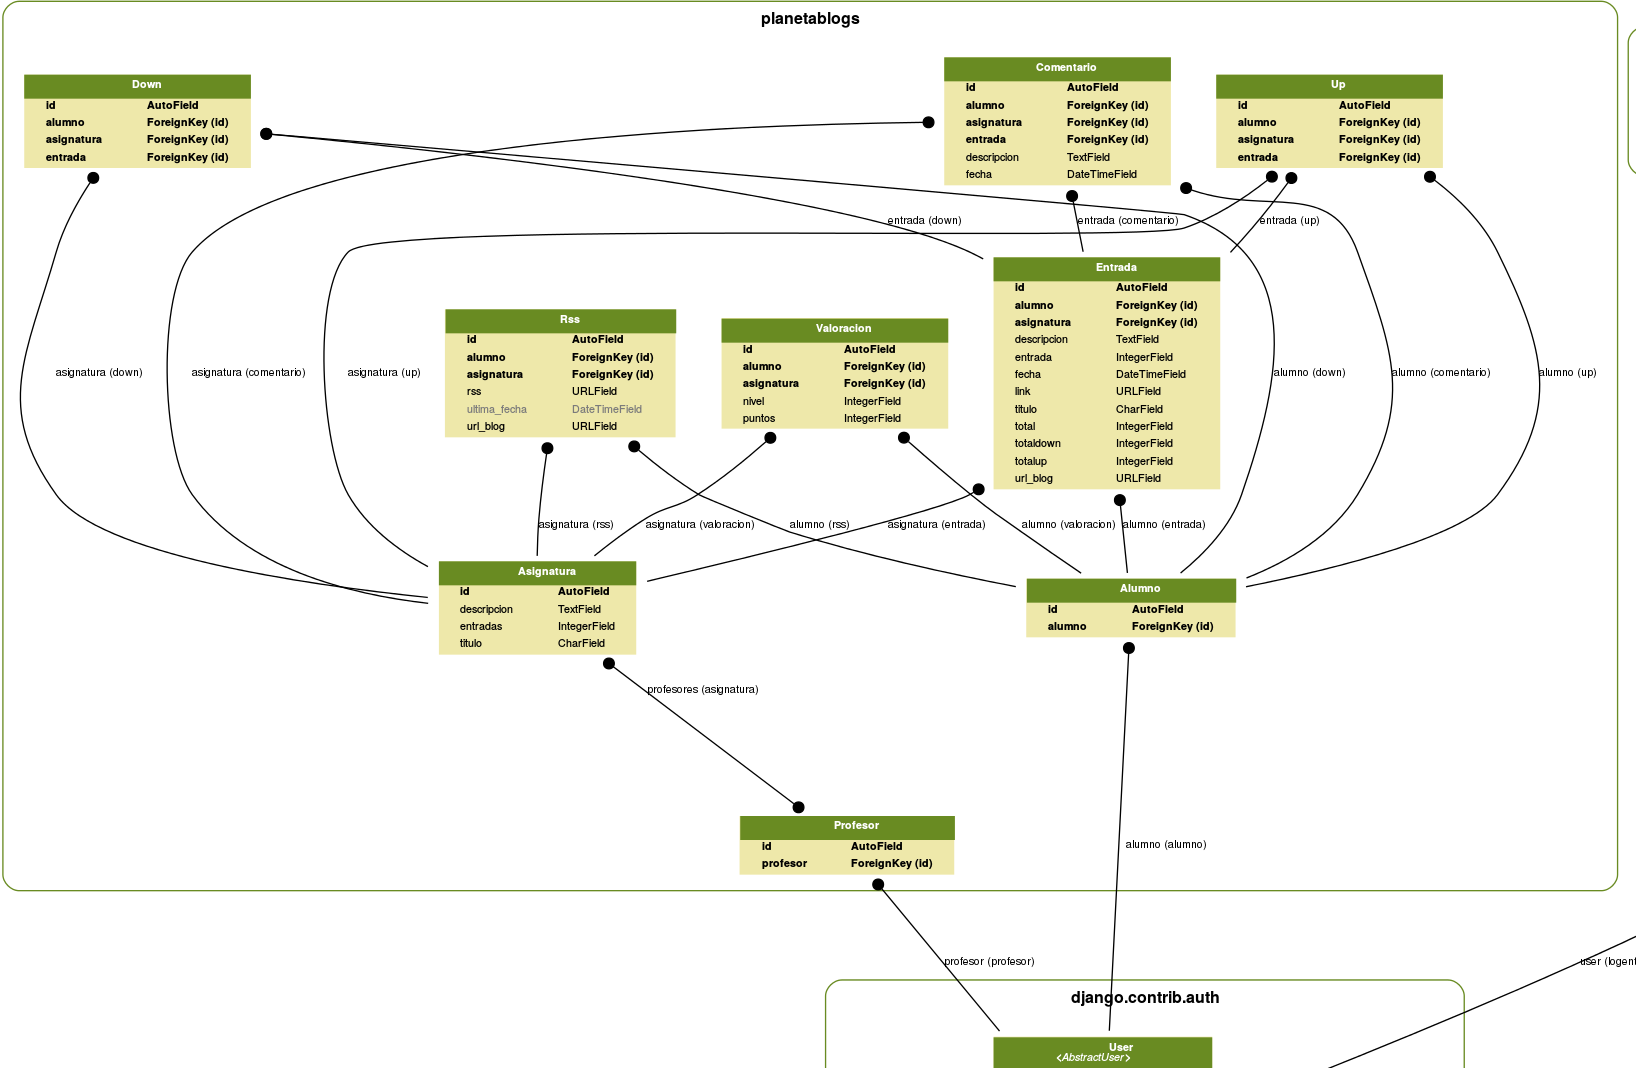
\includegraphics[width=17cm, keepaspectratio]{img/mis_modelos}}
  \caption{\textit{Estructura gr\'afica de la base de datos.}}
  \label{fig:disenobbdd}
\end{figure}


\subsection{Estructura de documentos \textit{HTML}} 
\label{sec:estructurahtml}
Todas las p\'aginas servidas por \texttt{Django} en este proyecto contienen en su cabecera (etiqueta \texttt{<head>}) las mismas referencias a ficheros 
\textit{JavaScript} y a ficheros \textit{CSS}. Estas referencias se vinculan con las tecnolog\'ias que ser\'an usadas dentro de los documentos \textit{HTML}:
Las bibliotecas \textit{JavaScript} de \textit{jQuery.js}, \textit{jQuery-ui.js} y \textit{BootStrap.js} son utilizadas para manejar distintas 
funcionalidades. Las bibliotecas \textit{CSS} de \textit{jQuery-ui.css} y \textit{BootStrap.css} son utilizadas para cambios en el dise\~no de la interfaz. 
Y por \'ultimo, los ficheros \textit{JavaScript} y \textit{CSS} propios de cada p\'agina que son utilizados para a\~nadir y mejorar tanto funcionalidad 
como dise\~no.

Dentro de la etiqueta \texttt{<body>} se introduce un elemento \texttt{<div>} con una clase \textit{.container} que mantiene una misma estructura en cada 
una de las p\'aginas:
\begin{itemize}
  \item {\bfseries Cabecera}: Dependiendo de la plantilla que se cargue en el cliente, la cabecera puede variar desde un mensaje de bienvenida a una barra
  de navegaci\'on.
  \item {\bfseries Contenedor}: En esta parte se muestra toda la informaci\'on con la que el usuario final podr\'a interactuar.
  \item {\bfseries Pie de p\'agina}: En todos los pies de p\'agina se muestra un correo electr\'onico como contacto y el nombre de la aplicaci\'on. 
  Las \'unicas p\'aginas que tienen pie de p\'agina son \texttt{index.html}, \texttt{ayuda.html} y las p\'aginas de registro.
\end{itemize}

\subsection{Dise\~no de las vistas y URLs} 
\label{sec:vistasurls}
Por la parte del servidor de un proyecto \texttt{Django} existe una parte importante que se encarga de procesar las solicitudes del cliente. Esta parte se
almacena en un fichero llamado \texttt{views.py}. Est\'a compuesto por vistas o funciones a las que \texttt{Django} accede despu\'es de que el usuario 
realice una petici\'on mediante una URL. El fichero \texttt{urls.py} define todas las URLs a las que se asociar\'a una vista distinta. A continuaci\'on
la vista procesa la solicitud y devuelve al cliente la informaci\'on pedida en forma de documento \textit{HTML} o \textit{JSON}.

Cada una de esas vistas se explican en las siguientes subsecciones:

\subsubsection{P\'agina de inicio} 
\label{sec:paginainicio}
El documento \textit{HTML} mostrado en la figura~\ref{fig:paginainicio} es la p\'agina de inicio. La p\'agina es servida tras una previa petici\'on \texttt{GET} del cliente 
mediante el correspondiente recurso \footnote{URL correspondiente a la p\'agina de inicio: \texttt{/planetablogs/login/}}. La vista asociada a ese recurso 
es \texttt{inicio}, la cual devuelve la plantilla \texttt{inicio.html} que crea el documento \textit{HTML} de la respuesta.

A esta p\'agina puede entrar cualquier usuario externo que pretenda crearse un perfil en la aplicaci\'on o quiera acceder a su perfil una vez creado.

En la cabecera se visualiza un mensaje de bienvenida animando a un ingreso en la aplicaci\'on. En el contenedor existen dos partes diferenciadas: 
\begin{itemize}
  \item {\bfseries \textit{Reg\'istrate}}: Se ofrece la posibilidad de darle a dos botones coloreados en verde, \textit{Alumno} o \textit{Tutor}. Debajo 
  de los botones se halla un mensaje explicativo que resumen la acci\'on de pulsar sobre ambos botones. Si se pulsa sobre el bot\'on \textit{Alumno} se 
  redirecciona a la p\'agina que se encarga de crear un perfil como alumno. Si se pulsa sobre el bot\'on \textit{Tutor} se redirecciona a la p\'agina que 
  se encarga de crear un perfil como tutor.
  \item {\bfseries \textit{Identif\'icate}}: En el formulario, una vez creado un usuario de aplicaci\'on, el usuario puede introducir sus datos 
  (\texttt{usuario} y \texttt{contrase\~na}) para identificarse y poder entrar a su perfil de usuario dentro de la aplicaci\'on. 
  
  Una vez se introducen los datos y el usuario pulsa en el bot\'on \textit{Aceptar}, el cliente realiza una petici\'on \texttt{POST} sobre la misma URL 
  por lo que ser\'a procesada por la misma vista \texttt{inicio}. Esta vista identifica la petici\'on como \texttt{POST}, almacena la informaci\'on enviada
  mediante el formulario, y la autentifica a trav\'es del proceso de autentificaci\'on de \texttt{Django} (\texttt{.authenticate}). Si el usuario est\'a 
  guardado en el modelo \texttt{User}, se ejecuta el proceso de login de \texttt{Django} (\texttt{.login}). A continuaci\'on se comprueba el tipo de usuario
  que se ha logado en la aplicaci\'on y dependiendo de si el tipo es \texttt{Alumno} o \texttt{Profesor}, la vista env\'ia una respuesta \texttt{HTTP} 
  redireccionando a la p\'agina de perfil del alumno o a la p\'agina de perfil del tutor, respectivamente. En el caso de que la informaci\'on sea incorrecta 
  la vista renderizar\'a la plantilla \texttt{inicio.html} con un mensaje de error de login.
\end{itemize}

\begin{figure}
  \centering
  \doublebox{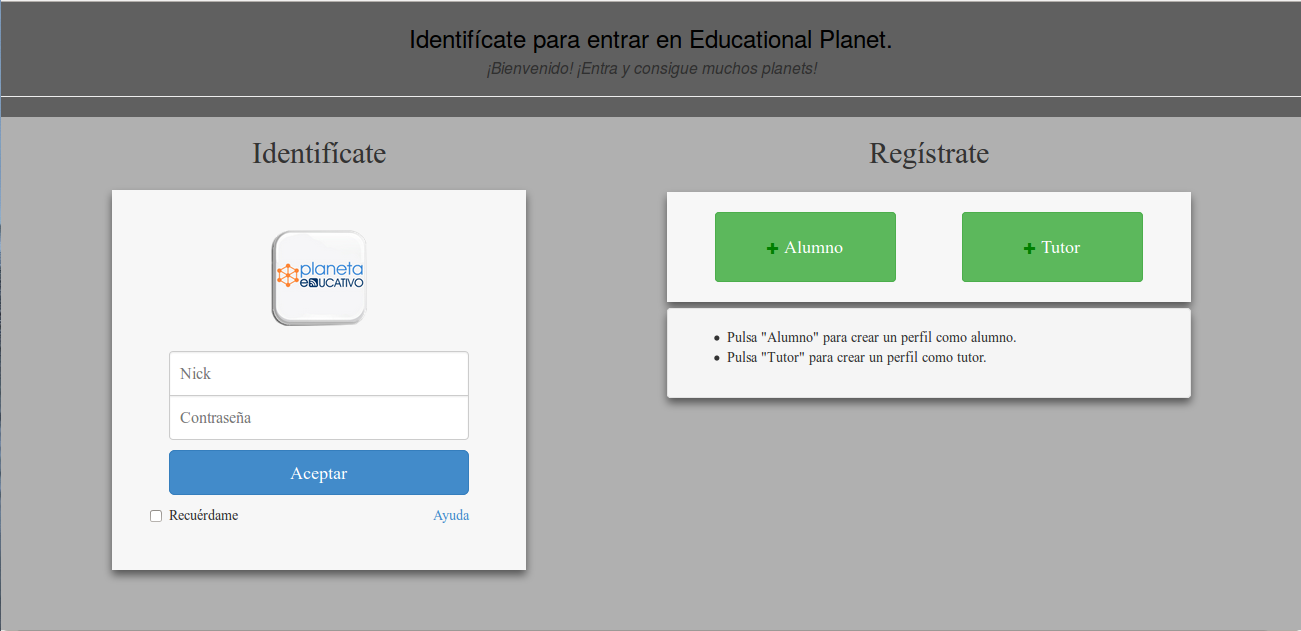
\includegraphics[width=17cm, keepaspectratio]{imagenes/PaginaInicio}}
  \caption{\textit{P\'agina de inicio.}}
  \label{fig:paginainicio}
\end{figure}


\subsubsection{Registro de alumno} 
\label{sec:registroalumno}
El documento \textit{HTML} mostrado en la figura~\ref{fig:registroalumno} es la p\'agina de registro realizado por parte de un alumno. La p\'agina es servida 
tras una previa petici\'on \texttt{GET} del cliente mediante el correspondiente recurso \footnote{URL correspondiente a la p\'agina de registro de un alumno: 
\texttt{/planetablogs/nuevoalumno/}}. La vista asociada a ese recurso es \texttt{nuevo\_alumno}, la cual devuelve la plantilla \texttt{nuevoalumno.html} 
que crea el documento \textit{HTML} de la respuesta.

A esta p\'agina puede acceder cualquier usuario externo que pretenda crearse un perfil en la aplicaci\'on.

En la cabecera se visualiza un mensaje informativo aclarando que el registro del perfil se crear\'a y guardar\'a como alumno. En el contenedor aparece un
formulario con la mayor\'ia de los campos del modelo \texttt{User} (\textit{Imagen}, \textit{Nick}, \textit{Nombre}, \textit{Apellidos}, \textit{Email} y 
\textit{Contrase\~na}).

Una vez relleno, el formulario se env\'ia pulsando sobre el bot\'on \texttt{Guardar} coloreado en verde. En ese momento, se realiza una petici\'on 
\texttt{POST} sobre la misma url por lo que ser\'a procesada por la misma vista \texttt{nuevo\_alumno}. Esta vista identifica la petici\'on como 
\texttt{POST}. La informaci\'on es enviada mediante un formulario de registro definido en \texttt{formularios.py}, y si este formulario es v\'alido, dicha
informaci\'on se almacena. La vista crea dos objetos, uno \texttt{User} y otro \texttt{Alumno}, y ambos los guarda en la base de datos. Y posteriormente, 
env\'ia una respuesta \texttt{HTTP} redireccionando a la p\'agina de inicio de la aplicaci\'on. En caso de que el formulario sea inv\'alido, la vista 
renderizar\'a la plantilla \texttt{nuevoalumno.html} con un mensaje de error de registro.

En caso de error de registro, te indicar\'a que puedes pasar el rat\'on por encima del icono de informaci\'on situado a la izquierda del bot\'on 
\texttt{Guardar}. Si esto sucede, mediante \textit{jQuery} y el evento \textit{.mouseover} en el fichero \texttt{nuevousuario.js}, se levanta un di\'alogo 
de informaci\'on que se encontraba previamente oculto.
\begin{figure}
  \centering
  \doublebox{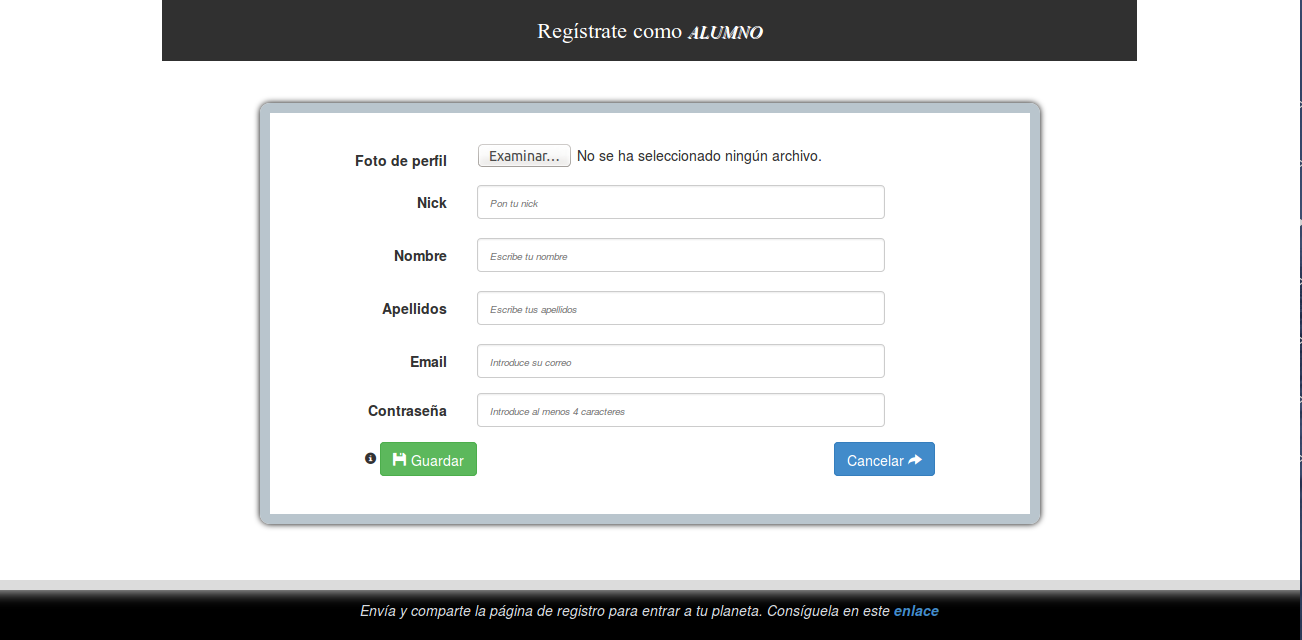
\includegraphics[width=17cm, keepaspectratio]{imagenes/RegistroAlumno}}
  \caption{\textit{P\'agina de registro de un alumno.}}
  \label{fig:registroalumno}
\end{figure}


\subsubsection{Registro de tutor} 
\label{sec:registrotutor}
El documento \textit{HTML} mostrado en la figura~\ref{fig:registrotutor} es la p\'agina de registro realizado por parte de un tutor. La p\'agina es servida 
tras una previa petici\'on \texttt{GET} del cliente mediante el correspondiente recurso \footnote{URL correspondiente a la p\'agina de registro de un alumno: 
\texttt{/planetablogs/nuevoprofesor/}}. La vista asociada a ese recurso es \texttt{nuevo\_profesor}, la cual devuelve la plantilla 
\texttt{nuevoprofesor.html} que crea el documento \textit{HTML} de la respuesta.

A esta p\'agina puede acceder cualquier usuario externo que pretenda crearse un perfil en la aplicaci\'on.

En la cabecera se visualiza un mensaje informativo aclarando que el registro del perfil se crear\'a y guardar\'a como tutor. En el contenedor aparece un
formulario con la mayor\'ia de los campos del modelo \texttt{User} (\textit{Imagen}, \textit{Nick}, \textit{Nombre}, \textit{Apellidos}, \textit{Email} y 
\textit{Contrase\~na}).

Una vez relleno, el formulario se env\'ia pulsando sobre el bot\'on \texttt{Guardar} coloreado en verde. En ese momento, se realiza una petici\'on 
\texttt{POST} sobre la misma URL por lo que ser\'a procesada por la misma vista \texttt{nuevo\_profesor}. Esta vista identifica la petici\'on como 
\texttt{POST}. La informaci\'on es enviada mediante un formulario de registro definido en \texttt{formularios.py}, y si este formulario es v\'alido, dicha
informaci\'on se almacena. La vista crea dos objetos, uno \texttt{User} y otro \texttt{Profesor}, y ambos los guarda en la base de datos. Y posteriormente, 
env\'ia una respuesta \texttt{HTTP} redireccionando a la p\'agina de inicio de la aplicaci\'on. En caso de que el formulario sea inv\'alido, la vista 
renderizar\'a la plantilla \texttt{nuevoprofesor.html} con un mensaje de error de registro.

En caso de error de registro, te indicar\'a que puedes pasar el rat\'on por encima del icono de informaci\'on situado a la izquierda del bot\'on 
\texttt{Guardar}. Si esto sucede, mediante \textit{jQuery} y el evento \textit{.mouseover} en el fichero \texttt{nuevousuario.js}, se levanta un di\'alogo 
de informaci\'on que se encontraba previamente oculto.
\begin{figure}
  \centering
  \doublebox{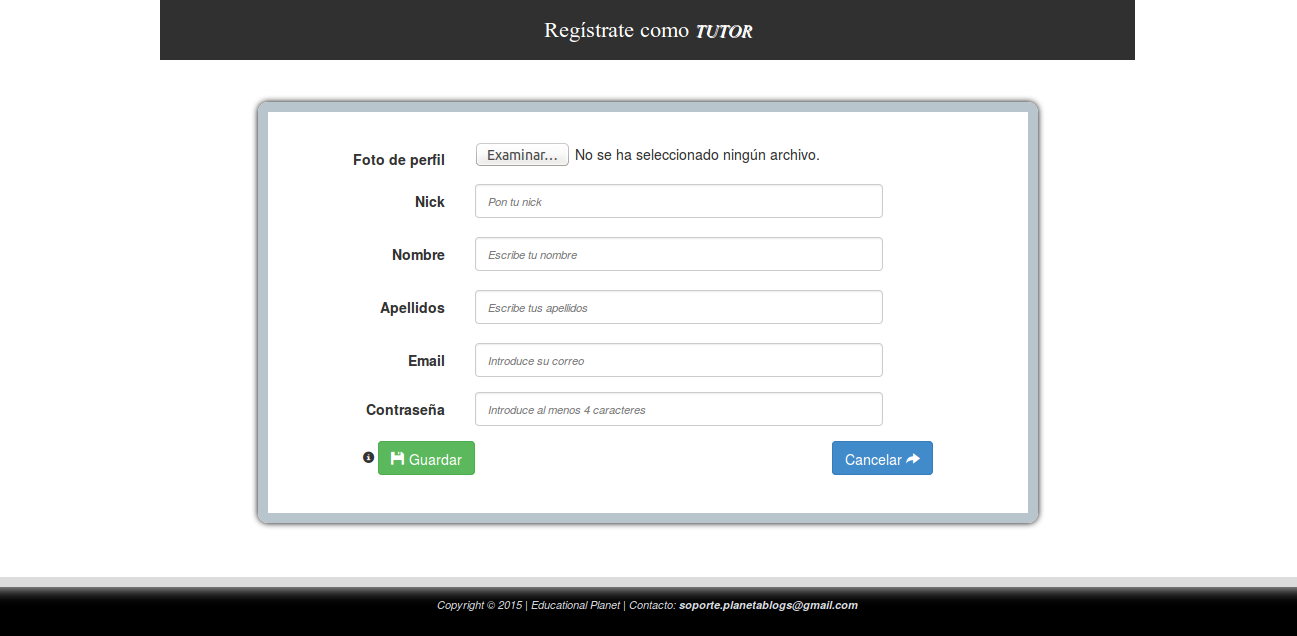
\includegraphics[width=17cm, keepaspectratio]{imagenes/RegistroTutor}}
  \caption{\textit{P\'agina de registro de un tutor.}}
  \label{fig:registrotutor}
\end{figure}


\subsubsection{Presentaci\'on de alumno} 
\label{sec:presentacionalumno}
El documento \textit{HTML} mostrado en la figura~\ref{fig:presentacionalumno} es la p\'agina de presentaci\'on del perfil de un alumno. La p\'agina es servida 
tras una previa petici\'on \texttt{GET} del cliente mediante el correspondiente recurso \footnote{URL correspondiente a la p\'agina de registro de un alumno: 
\texttt{/planetablogs/alumnos/}}. La vista asociada a ese recurso es \texttt{presentacionalumno}, la cual devuelve la plantilla 
\texttt{presentacionalum.html} que crea el documento \textit{HTML} de la respuesta.

A esta p\'agina solamente puede acceder un usuario que se haya registrado previamente en la aplicaci\'on, y adem\'as lo haya hecho como alumno.

En la parte superior de la cabecera se encuentra la barra de navegaci\'on con dos enlaces. \texttt{Mis hilos} hace referencia a la misma URL de la 
p\'agina servida, por lo que la recargar\'a, y \texttt{Desconectar} para el cierre de la sesi\'on (Secci\'on~\ref{sec:cierresesion}). En la parte inferior 
de la cabecera se muestra una foto de perfil y un mensaje que informa a quien pertenece el espacio de la sesi\'on.

Dentro del contenedor hay que destacar dos partes importantes:
\begin{itemize}
  \item {\bfseries \texttt{Hilos disponibles}}: Aparecen todas las asignaturas disponibles a las que se puede suscribir el alumno. Cada formulario 
  corresponde con una asignatura de la cual se muestra su t\'itulo y su descripci\'on. El campo del formulario se debe rellenar con un RSS v\'alido antes 
  de enviarlo pulsando sobre el bot\'on \texttt{Guardar y a\~nadir} coloreado en naranja. En ese instante, se realiza una petici\'on 
  \texttt{POST} sobre la misma URL por lo que ser\'a procesada por la misma vista \texttt{presentacionalumno}. Esta vista identifica la petici\'on como 
  \texttt{POST}. La informaci\'on es enviada mediante un formulario (\textit{FormularioAgregarRSS}) definido en \texttt{formularios.py}. La vista valida 
  el formulario de tal forma que cumpla que la URL del RSS tiene que ser correcta y no estar ocupada por ninguna asignatura de ning\'un alumno registrado 
  en la aplicaci\'on. La vista crea un objeto en la tabla del modelo \texttt{RSS} en base de datos con el dato introducido en el formulario y una fecha que 
  marca el inicio de la actividad de ese RSS. Adem\'as, la vista crea otro objeto en el modelo \texttt{Valoracion} para inicializar la puntuaci\'n y el 
  nivel de ese alumno en esa asignatura. Por \'ultimo, se env\'ia una respuesta \texttt{HTTP} redireccionando a la p\'agina de presentaci\'on del alumno. 
  En caso de que el formulario sea inv\'alido, la vista renderizar\'a la plantilla \texttt{presentacionalum.html} con un mensaje de error de dato 
  introducido.
  \item {\bfseries \texttt{Mis hilos}}: La vista busca por el \texttt{ID} del alumno y filtra las asignaturas a las que est\'a suscrito ese alumno para 
  imprimirlas posteriormente a la hora de renderizar la plantilla \texttt{presentacionalum.html}.
\end{itemize}

\begin{figure}
  \centering
  \doublebox{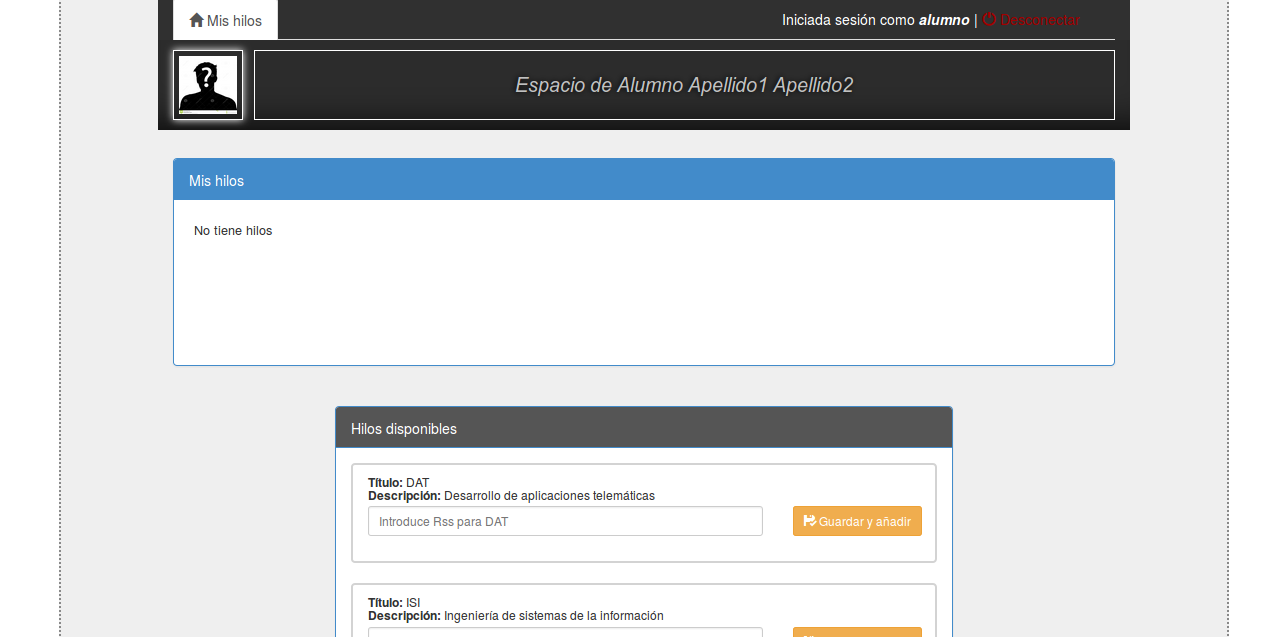
\includegraphics[width=17cm, keepaspectratio]{imagenes/PresentacionAlumno}}
  \caption{\textit{Presentaci\'on del perfil de un alumno.}}
  \label{fig:presentacionalumno}
\end{figure}


\subsubsection{Presentaci\'on de tutor}
\label{sec:presentaciontutor}
El documento \textit{HTML} mostrado en la figura~\ref{fig:presentaciontutor} es la p\'agina de presentaci\'on del perfil de un tutor. La p\'agina es servida 
tras una previa petici\'on \texttt{GET} del cliente mediante el correspondiente recurso \footnote{URL correspondiente a la p\'agina de registro de un alumno: 
\texttt{/planetablogs/tutores/}}. La vista asociada a ese recurso es \texttt{presentacionprofesor}, la cual devuelve la plantilla 
\texttt{presentacionprof.html} que crea el documento \textit{HTML} de la respuesta.

A esta p\'agina solamente puede acceder un usuario que se haya registrado previamente en la aplicaci\'on, y adem\'as lo haya hecho como profesor.

En la parte superior de la cabecera se encuentra la barra de navegaci\'on con dos enlaces. \texttt{Mis hilos} hace referencia a la misma URL de la 
p\'agina servida, por lo que la recargar\'a, \texttt{Resetear contrase\~na} hace referencia a la URL de cambio de contrase\~na y \texttt{Desconectar} para el cierre de la sesi\'on (Secci\'on~\ref{sec:cierresesion}). En la parte inferior 
de la cabecera se muestra una foto de perfil y un mensaje que informa a quien pertenece el espacio de la sesi\'on.

Dentro del contenedor hay que destacar tres partes importantes:
\begin{itemize}
  \item {\bfseries \texttt{Crear hilo}}: Es un bot\'on que despliega un formulario a trav\'es de un efecto \texttt{toggle} de \textit{jQuery-ui}. Este 
  formulario introduce dos campos, t\'itulo y descripci\'on, que definen un objeto del modelo \texttt{Asignatura}. Se env\'ia pulsando sobre el bot\'on
  \texttt{Enviar} y se realiza una petici\'on \texttt{POST} sobre la misma URL por lo que ser\'a procesada por la misma vista \texttt{presentacionprofesor}.
  Esta vista identifica la petici\'on como \texttt{POST}. La informaci\'on es enviada mediante un formulario (\textit{FormularioHilo}) definido en 
  \texttt{formularios.py}. La vista valida el formulario y crea un objeto en la tabla del modelo \texttt{Asignatura} en base de datos con los dos datos 
  introducidos en el formulario y un campo \texttt{entradas} que inicializa el n\'umero de entradas totales existentes en ese hilo. Se renderiza 
  la plantilla \texttt{presentacionprof.html} en la respuesta a la petici\'on la cual redirecciona a la p\'agina de presentaci\'on del profesor. 
  \item {\bfseries \texttt{Hilos disponibles}}: Aparecen todas las asignaturas disponibles a las que puede seguir el profesor, sin contar las asignaturas
  agregadas a su secci\'on de \texttt{Mis hilos}.
  \item {\bfseries \texttt{Mis hilos}}: La vista busca por el \texttt{ID} del profesor y filtra las asignaturas a las que sigue ese profesor para 
  imprimirlas posteriormente a la hora de renderizar la plantilla \texttt{presentacionprof.html}.
\end{itemize}

\begin{figure}
  \centering
  \doublebox{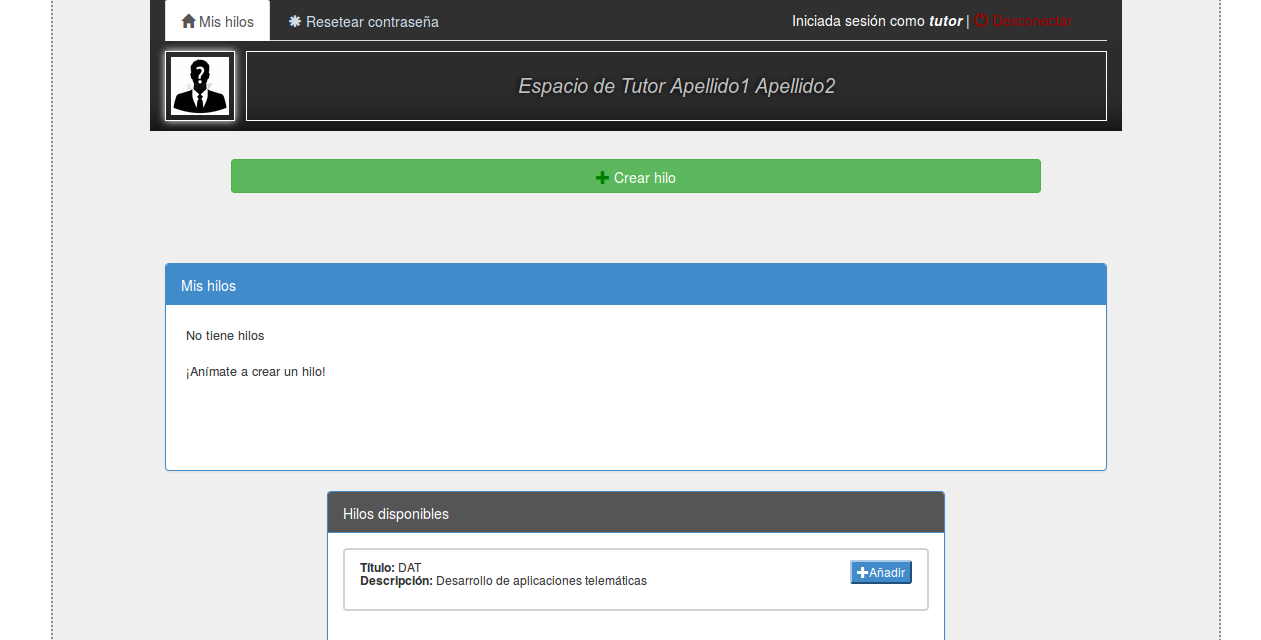
\includegraphics[width=17cm, keepaspectratio]{imagenes/PresentacionTutor}}
  \caption{\textit{Presentaci\'on del perfil de un tutor.}}
  \label{fig:presentaciontutor}
\end{figure}


\subsubsection{Resetear contrase\~na} 
\label{sec:resetpass}
El documento \textit{HTML} mostrado en la figura~\ref{fig:resetpass} es la p\'agina de modificaci\'on de contrase\~na. La p\'agina es servida 
tras una previa petici\'on \texttt{GET} del cliente mediante el correspondiente recurso \footnote{URL correspondiente a la p\'agina de resetear contrase\~na: 
\texttt{/planetablogs/tutores/resetear\_password/}}. La vista asociada a ese recurso es \texttt{resetear\_password}, la cual devuelve la plantilla 
\texttt{resetear\_password.html} que crea el documento \textit{HTML} de la respuesta.

A esta p\'agina solamente puede acceder un usuario que se haya registrado previamente en la aplicaci\'on, y adem\'as lo haya hecho como profesor. 

En la parte superior de la cabecera se encuentra la barra de navegaci\'on con tres enlaces. \texttt{Resetear contrase\~na} hace referencia a la misma 
URL de la p\'agina servida, por lo que la recargar\'a, \texttt{Mis hilos} hace referencia a la URL del perfil del tutor y \texttt{Desconectar} para 
el cierre de la sesi\'on (Secci\'on~\ref{sec:cierresesion}).

En el cuerpo del documento existe un formulario en el que el alumno que haya perdido u olvidado su contrase\~na, puede introducir su nick de usuario y una
nueva contrase\~na que sustituir\'a a la anterior.

\begin{figure}
  \centering
  \doublebox{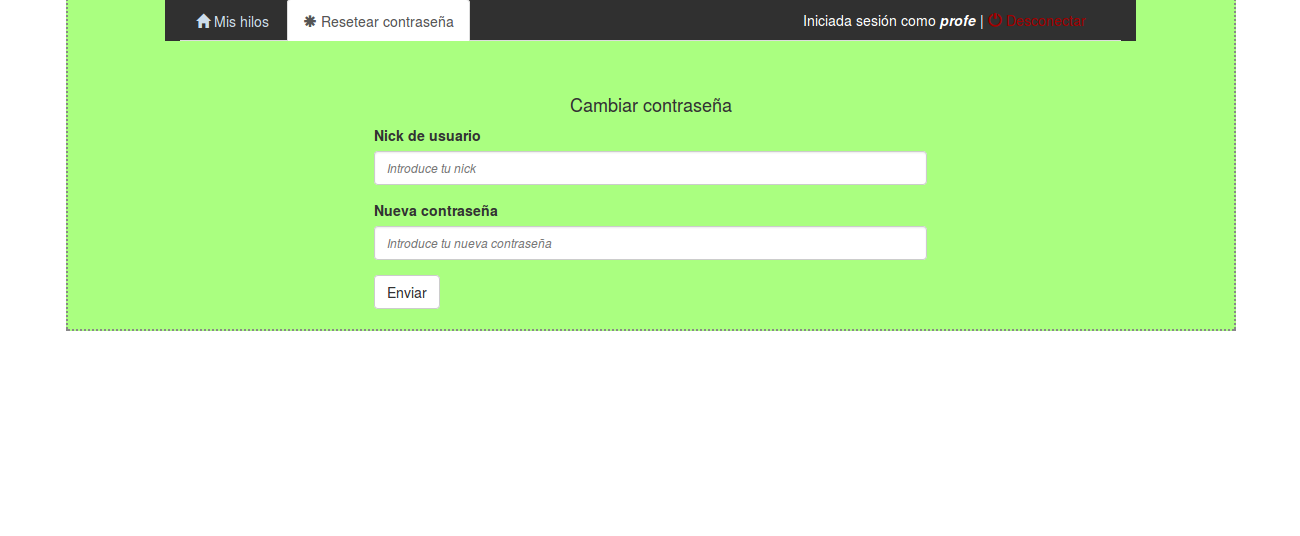
\includegraphics[width=17cm, keepaspectratio]{imagenes/ResetPass}}
  \caption{\textit{Modificar una contrase\~na desde el perfil de un tutor.}}
  \label{fig:resetpass}
\end{figure}




\subsubsection{Hilos} 
\label{sec:hilos}
En la figura~\ref{fig:hilos} se muestran dos documentos \textit{HTML} que recogen el contenido de un hilo. En la figura~\ref{fig:hilos}(a) se visualiza el interior
de un hilo limpio, sin entradas, en la parte del alumno. En la figura~\ref{fig:hilos}(b) se visualiza el interior del mismo hilo limpio en la parte del 
tutor. La diferencia entre ambas im\'agenes se explicar\'a en las dos pr\'oximas subsecciones.

La cabecera de ambas im\'agenes se pueden observar los distintos \'items de la barra de navegaci\'on. La barra de navegaci\'on ser\'a la misma dentro de
todas las plantillas con la siguiente URL: {\scriptsize \texttt{/planetablogs/alumnos/hilo/\textit(IdAsignatura)/[\textit(buscar),\textit(puntuaciones),
\textit(infopuntuaciones)]}}
\begin{itemize}
  \item {\bfseries \textit{Mis hilos}}: Es un enlace que hace referencia a la URL de la presentaci\'on del perfil de usuario 
  (Secci\'on~\ref{sec:presentacionalumno}).
  \item {\bfseries \textit{Asignatura}}: Enlace que hace referencia a la misma URL de la p\'agina servida, por lo que la recargar\'a (en este caso, 
  la asignatura se llama \texttt{DAT}).
  \item {\bfseries \textit{Buscar}}: Es un enlace que hace referencia a la URL de b\'usqueda (Secci\'on~\ref{sec:buscar}).
  \item {\bfseries \textit{Puntuaciones}}: Es una lista desplegable compuesta por tres enlaces. \textit{Ranking} hace referencia a la URL donde se muestran 
  todas las puntuaciones de los usuarios de un determinado hilo. \textit{Estad\'isticas} hace referencia a la URL donde se muestran las estad\'isticas de 
  cada usuario de un determinado hilo, tanto estad\'isticas generales como resumen de entradas. \textit{Informaci\'on} hace referencia a la URL que 
  recoge las bases de esas puntuaciones.
  \item {\bfseries \textit{Desconectar}}: Enlace que hace referencia a la URL servida para el cierre de la sesi\'on (Secci\'on~\ref{sec:cierresesion}).
\end{itemize}
Tambi\'en se expone, debajo de la barra de navegaci\'on, una imagen correspondiente al logo de la aplicaci\'on con su t\'itulo. Y en la parte derecha un 
apartado que agrupa las entradas m\'as valoradas del hilo.

\begin{figure}
  \centering
  \subfigure[Hilo limpio en alumno]{\doublebox{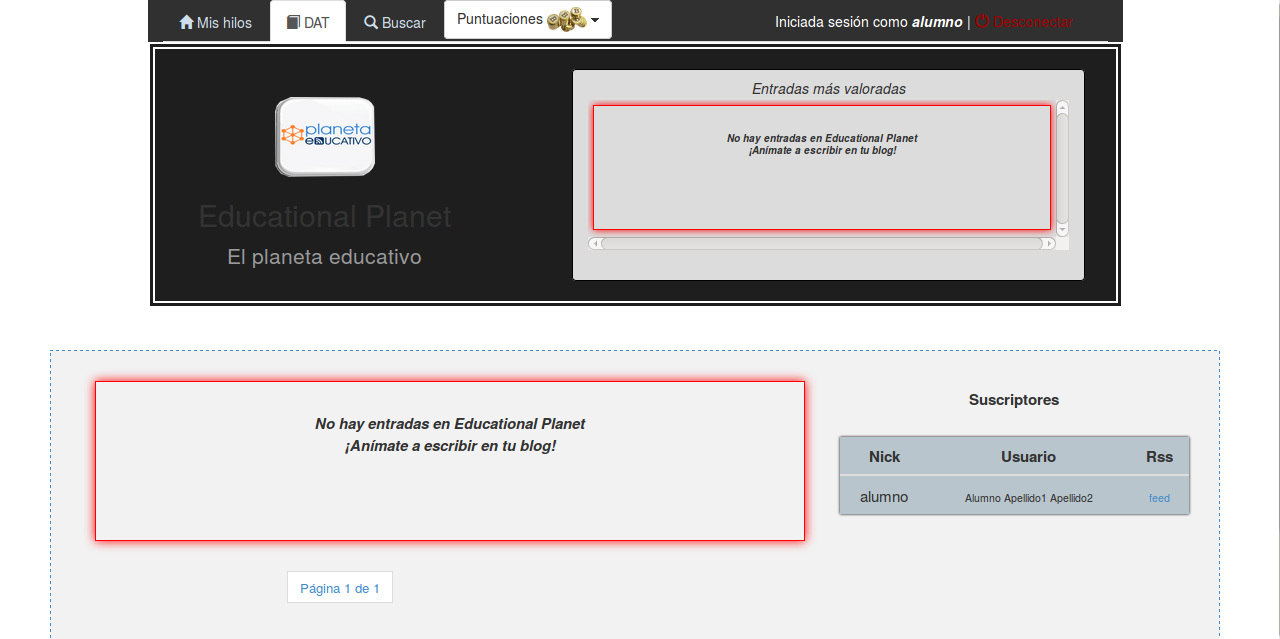
\includegraphics[width=7cm]{imagenes/HiloAlumno}}}
  \subfigure[Hilo limpio en tutor]{\doublebox{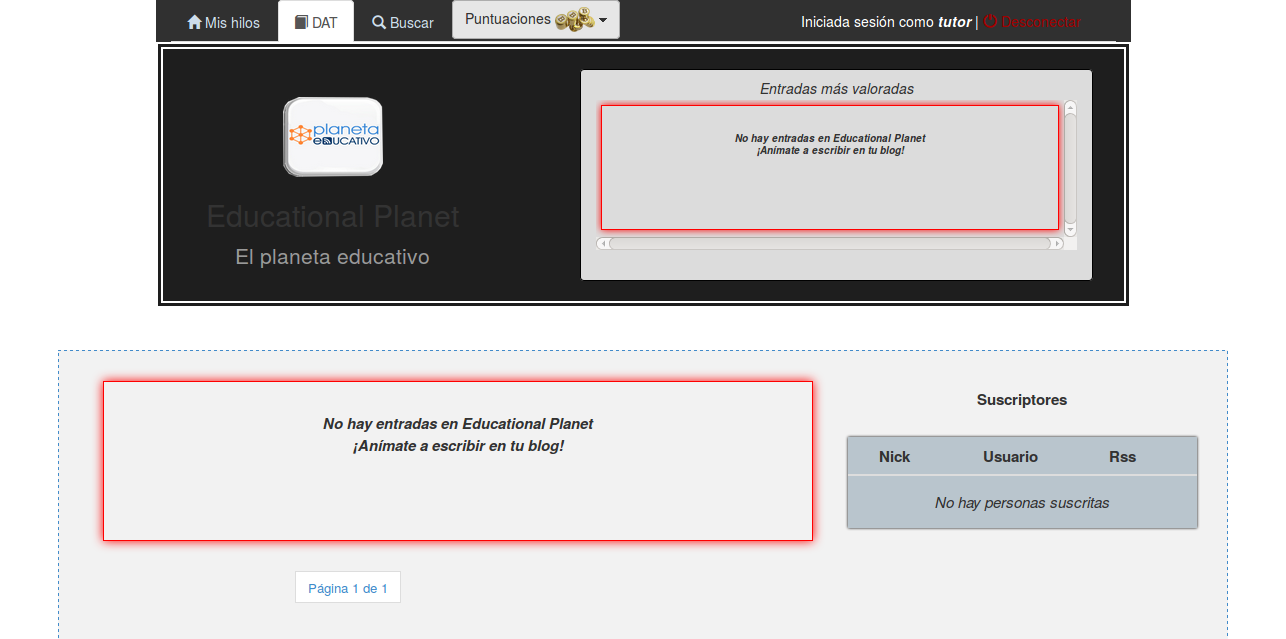
\includegraphics[width=7cm]{imagenes/HiloTutor}}}
  \caption{\textit{P\'agina principal de un hilo limpio.}}
  \label{fig:hilos}
\end{figure}


\subsubsection{Hilo de alumno} 
\label{sec:hiloalumno}
El documento \textit{HTML} mostrado en la figura~\ref{fig:hiloalumno} es el contenedor de la p\'agina de un determinado hilo al que est\'a suscrito un alumno. 
La p\'agina es servida tras una previa petici\'on \texttt{GET} del cliente mediante el correspondiente recurso \footnote{URL correspondiente al hilo al que est\'a
suscrito un alumno: \texttt{/planetablogs/alumnos/hilo/\textit(IdAsignatura)}}. La vista asociada a ese recurso es \texttt{mostrarhiloalumno}, la cual 
devuelve la plantilla \texttt{index.html} que crea el documento \textit{HTML} de la respuesta.

A esta p\'agina solamente puede acceder un usuario que se haya registrado previamente en la aplicaci\'on como alumno y que est\'e suscrito a la
correspondiente asignatura de inter\'es.

La vista filtra por el usuario conectado y por el Id de la asignatura pasada como argumento en el recurso de la petici\'on, para obtener la lista de 
usuarios, la lista de comentarios, la lista de entradas m\'as valoradas, y la lista de entradas pertenecientes a esa asignatura. 
El contenedor de la plantilla expone la lista de entradas tal y como se muestra en la figura. En la parte derecha del contenedor se re\'une la lista de 
usuarios suscritos a este hilo. Cabe destacar que la lista de entradas dentro del contenedor est\'a limitada por un paginador creado por la vista. Cada 
p\'agina dentro del hilo mostrar\'a en su contenedor cinco entradas como m\'aximo. El orden de la lista de entradas est\'a colocado de menor a mayor por 
antiguedad, siendo las primeras entradas visibles las m\'as recientes.

La respuesta de la vista tambi\'en contiene cinco estructuras \textit{JSON}, todos los usuarios del modelo \texttt{User} (\textit{json\_usuarios}), 
todas las valoraciones del modelo \texttt{Valoracion} pertenecientes a ese hilo (\textit{json\_valoracion}), todos los alumnos del modelo \texttt{Alumno} 
(\textit{json\_alumnos}), todas las asignaturas del modelo \texttt{Asignatura} (\textit{json\_asignaturas}), todos los profesores del modelo \texttt{Profesor} 
(\textit{json\_profesores}).

\begin{figure}
  \centering
  \Ovalbox{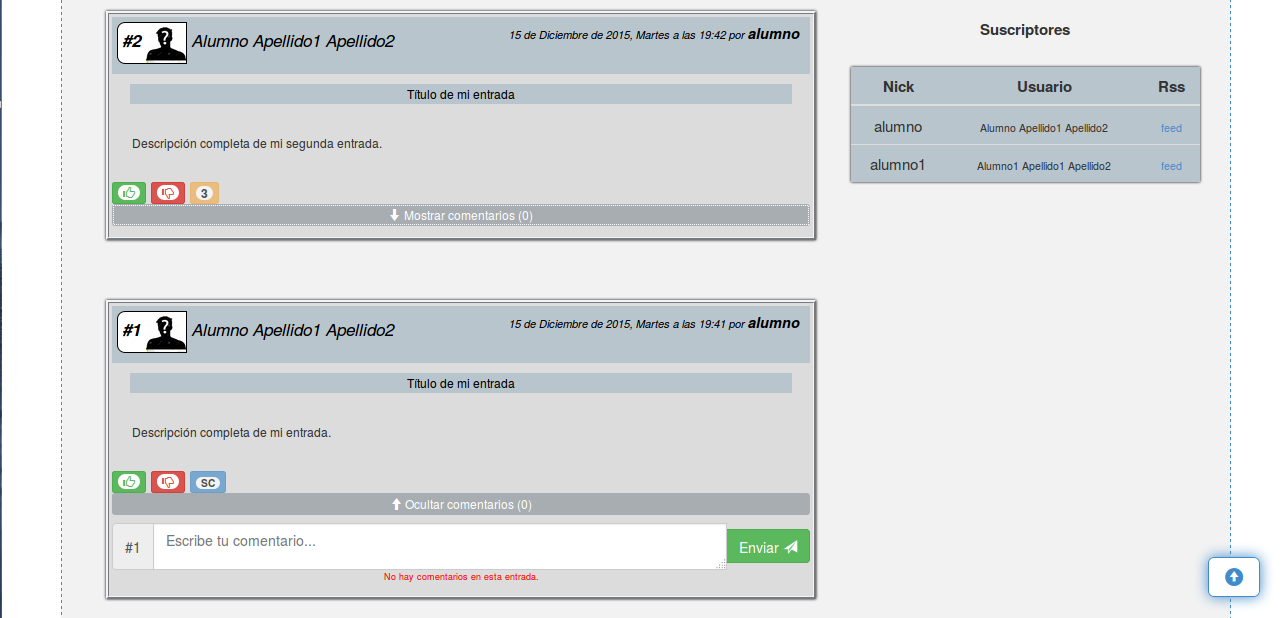
\includegraphics[width=17cm, keepaspectratio]{imagenes/HiloAlumnoEntradas}}
  \caption{\textit{P\'agina principal de un hilo de un alumno.}}
  \label{fig:hiloalumno}
\end{figure}


\subsubsection{Hilo de tutor} 
\label{sec:hilotutor}
El documento \textit{HTML} mostrado en la figura~\ref{fig:hilotutor} es el contenedor de la p\'agina de un determinado hilo al que est\'a suscrito un tutor. 
La p\'agina es servida tras una previa petici\'on \texttt{GET} del cliente mediante el correspondiente recurso \footnote{URL correspondiente al hilo al que est\'a
suscrito un tutor: \texttt{/planetablogs/tutores/hilo/\textit(IdAsignatura)}}. La vista asociada a ese recurso es \texttt{mostrarhiloprofesor}, la cual 
devuelve la plantilla \texttt{index\_tutor.html} que crea el documento \textit{HTML} de la respuesta.

A esta p\'agina solamente puede acceder un usuario que se haya registrado previamente en la aplicaci\'on como profesor y que est\'e suscrito a la
correspondiente asignatura de inter\'es.

La vista filtra por el Id de la asignatura pasada como argumento en el recurso de la petici\'on, para obtener la lista de 
usuarios, la lista de comentarios, la lista de entradas m\'as valoradas, y la lista de entradas pertenecientes a esa asignatura. 
El contenedor de la plantilla expone la lista de entradas tal y como se muestra en la figura. En la parte derecha del contenedor se re\'une la lista de 
usuarios suscritos a este hilo. Cabe destacar que la lista de entradas dentro del contenedor est\'a limitada por un paginador creado por la vista. Cada 
p\'agina dentro del hilo mostrar\'a en su contenedor cinco entradas como m\'aximo. El orden de la lista de entradas est\'a colocado de menor a mayor por 
antiguedad, siendo las primeras entradas visibles las m\'as recientes.

La respuesta de la vista tambi\'en contiene cinco estructuras \textit{JSON}, todos los usuarios del modelo \texttt{User} (\textit{json\_usuarios}), 
todas las valoraciones del modelo \texttt{Valoracion} pertenecientes a ese hilo (\textit{json\_valoracion}), todos los alumnos del modelo \texttt{Alumno} 
(\textit{json\_alumnos}), todas las asignaturas del modelo \texttt{Asignatura} (\textit{json\_asignaturas}), todos los profesores del modelo \texttt{Profesor} 
(\textit{json\_profesores}).

La principal diferencia con las p\'aginas de los hilos mostrados por parte de los alumnos, es que los tutores tienen el permiso de eliminar entradas de la 
lista de entradas o usuarios de la lista de usuarios, y adem\'as pueden puntuar de forma cuantitativa cada entrada.

\begin{figure}
  \centering
  \Ovalbox{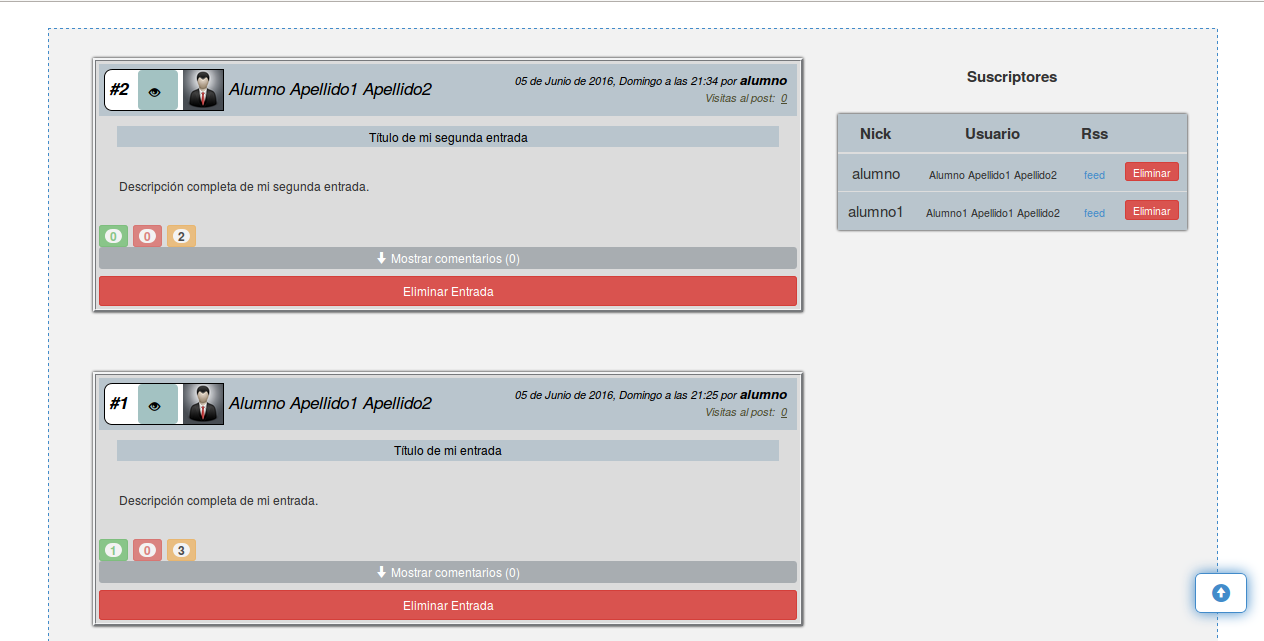
\includegraphics[width=17cm, keepaspectratio]{imagenes/HiloTutorEntradas}}
  \caption{\textit{P\'agina principal de un hilo de un tutor.}}
  \label{fig:hilotutor}
\end{figure}


\subsubsection{B\'usqueda avanzada} 
\label{sec:buscar}
El documento \textit{HTML} mostrado en la figura~\ref{fig:buscar} pertenece la p\'agina de b\'usqueda avanzada de entradas. 
La p\'agina es servida tras una previa petici\'on \texttt{GET} del cliente mediante el correspondiente recurso \footnote{URL correspondiente a la p\'agina de 
b\'usqueda: \texttt{/planetablogs/tutores/hilo/\textit(IdAsignatura)/buscar/}}. La vista asociada a ese recurso es \texttt{buscar}, la cual 
devuelve la plantilla \texttt{buscar.html} que crea el documento \textit{HTML} de la respuesta.

A esta p\'agina solamente puede acceder un usuario que se haya registrado previamente en la aplicaci\'on y que est\'e suscrito a la correspondiente 
asignatura de inter\'es.

La cabecera re\'une todos los \'items de la barra de navegaci\'on explicada en la secci\'on~\ref{sec:hilos}. La parte del documento de la clase 
\textit{.container} crea un formulario con una etiqueta \texttt{<select>} la cual despliega dos opciones de b\'usqueda a elegir, por \textit{Nick de usuario} 
y por \textit{Id de entrada}.
\begin{figure}
  \centering
  \doublebox{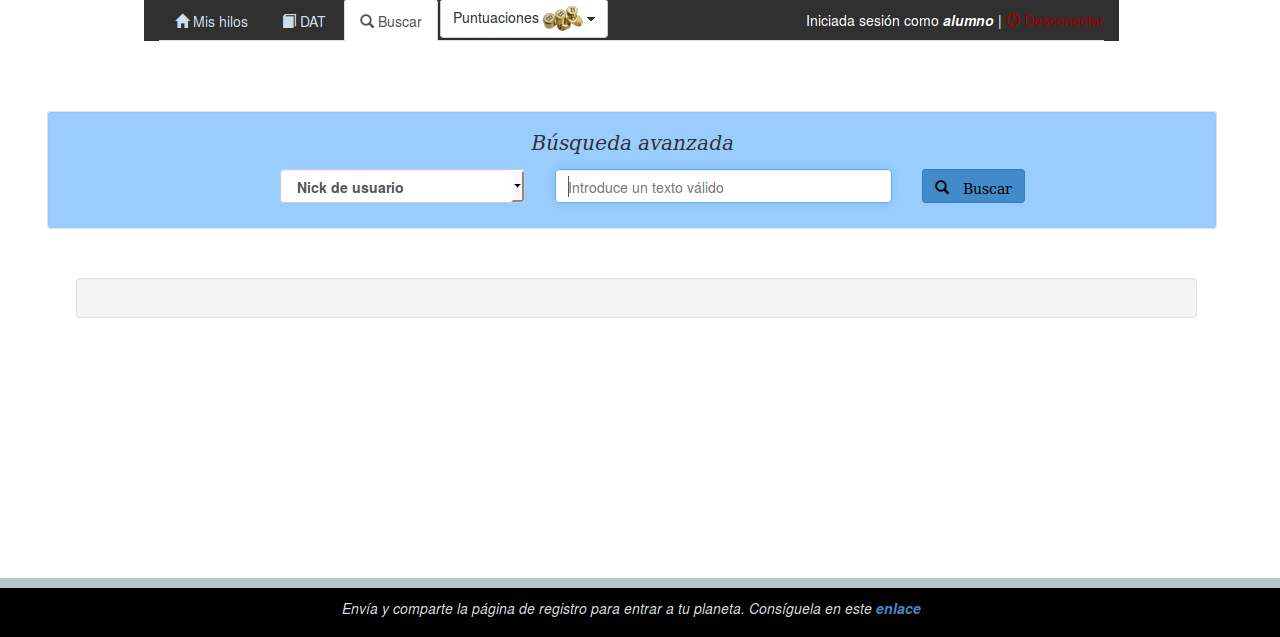
\includegraphics[width=17cm, keepaspectratio]{imagenes/HiloAlumnoBuscar}}
  \caption{\textit{P\'agina de b\'usqueda avanzada de entradas.}}
  \label{fig:buscar}
\end{figure}


\subsubsection{Ranking} 
\label{sec:ranking}
El documento \textit{HTML} mostrado en la figura~\ref{fig:ranking} corresponde con la p\'agina de ranking de un determinado hilo. 
La p\'agina es servida tras una previa petici\'on \texttt{GET} del cliente mediante el correspondiente recurso \footnote{URL correspondiente a la p\'agina de 
ranking: \texttt{/planetablogs/tutores/hilo/\textit(IdAsignatura)/puntuaciones/}}. La vista asociada a ese recurso es \texttt{puntuaciones}, la cual 
devuelve la plantilla \texttt{puntuaciones.html} que crea el documento \textit{HTML} de la respuesta.

A esta p\'agina solamente puede acceder un usuario que se haya registrado previamente en la aplicaci\'on y que est\'e suscrito a la
correspondiente asignatura de inter\'es.

La cabecera re\'une todos los \'items de la barra de navegaci\'on explicada en la secci\'on~\ref{sec:hilos}. 

La vista \texttt{puntuaciones} recibe como par\'ametro el Id del hilo, y mediante ese Id procesa la petici\'on obteniendo la asignatura y la lista 
de valoraciones asociadas a esa asignatura. Serializa una lista \textit{JSON} con todos los objetos del modelo \texttt{User} (\textit{json\_usuarios}).
Toda esa informaci\'on es enviada como respuesta a la solicitud en la plantilla \texttt{puntuaciones.html}. 

Por lo que, la parte del documento \textit{HTML} de la clase \textit{.container} agrupa todos los usuarios de una asignatura en una tabla \textit{HTML} (etiqueta 
\texttt{<table>}) con varios elementos de informaci\'on: \textit{Posici\'on}, \textit{Usuario}, \textit{Planets} y \textit{Nivel}.

\begin{figure}
  \centering
  \doublebox{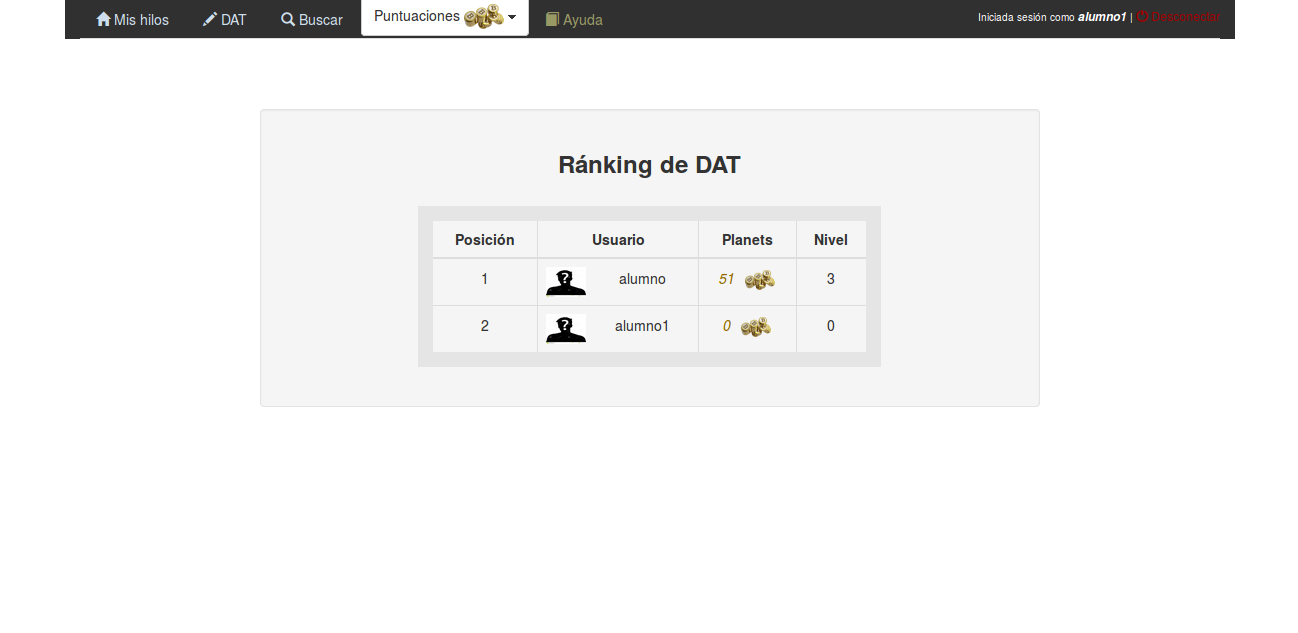
\includegraphics[width=17cm, keepaspectratio]{imagenes/HiloAlumnoRanking}}
  \caption{\textit{P\'agina de ranking.}}
  \label{fig:ranking}
\end{figure}


\subsubsection{Estad\'isticas} 
\label{sec:estadisticas}
El documento \textit{HTML} mostrado en la figura~\ref{fig:estadisticas} corresponde con la p\'agina de estad\'isticas de un determinado hilo. 
La p\'agina es servida tras una previa petici\'on \texttt{GET} del cliente mediante el correspondiente recurso \footnote{URL correspondiente a la p\'agina de 
ranking: \texttt{/planetablogs/tutores/hilo/\textit(IdAsignatura)/estadisticas/}}. La vista asociada a ese recurso es \texttt{estadisticas}, la cual 
devuelve la plantilla \texttt{estadisticas.html} que crea el documento \textit{HTML} de la respuesta.

A esta p\'agina solamente puede acceder un usuario que se haya registrado previamente en la aplicaci\'on y que est\'e suscrito a la
correspondiente asignatura de inter\'es.

La cabecera re\'une todos los \'items de la barra de navegaci\'on explicada en la secci\'on~\ref{sec:hilos}. 

La vista \texttt{estadisticas} recibe como par\'ametro el Id del hilo, y mediante ese Id procesa la petici\'on obteniendo la asignatura, la lista 
de entradas asociadas a esa asignatura y una lista de listas que recoge informaci\'on de cada alumno (datos personales, total de entradas, total de up 
recibidos, total de down recibidos, total up enviados, total down enviados, total comentarios recibidos y total comentarios enviados).

Toda esa informaci\'on es enviada como respuesta a la solicitud en la plantilla \texttt{estadisticas.html}. 

Por lo que, la parte del documento \textit{HTML} de la clase \textit{.container} agrupa todos los usuarioS de una asignatura en un acorde\'on (elemento 
\textit{jQuery-ui}). Cada secci\'on del acorde\'on pertenece a un usuario y muestra dos tablas (elemento \texttt{<table>}): \textit{Estad\'isticas 
generales del alumno} y \textit{Entradas del alumno}, con informaci\'on recopilada y organizada. 

En la parte superior del cuerpo de la p\'agina, mediante \textit{radiobuttons} se da la opci\'on de elegir lo que queremos mostrar. Al clicar sobre cada 
radiobutton, mediante los eventos \textit{jQuery}, \textit{hide()} y \textit{show()}, 
escritos en el fichero estadisticas.js, se oculta o se muestra la tabla de estad\'isticas de usuario, la tabla de resumen de entradas o ambas tablas.

\begin{figure}
  \centering
  \doublebox{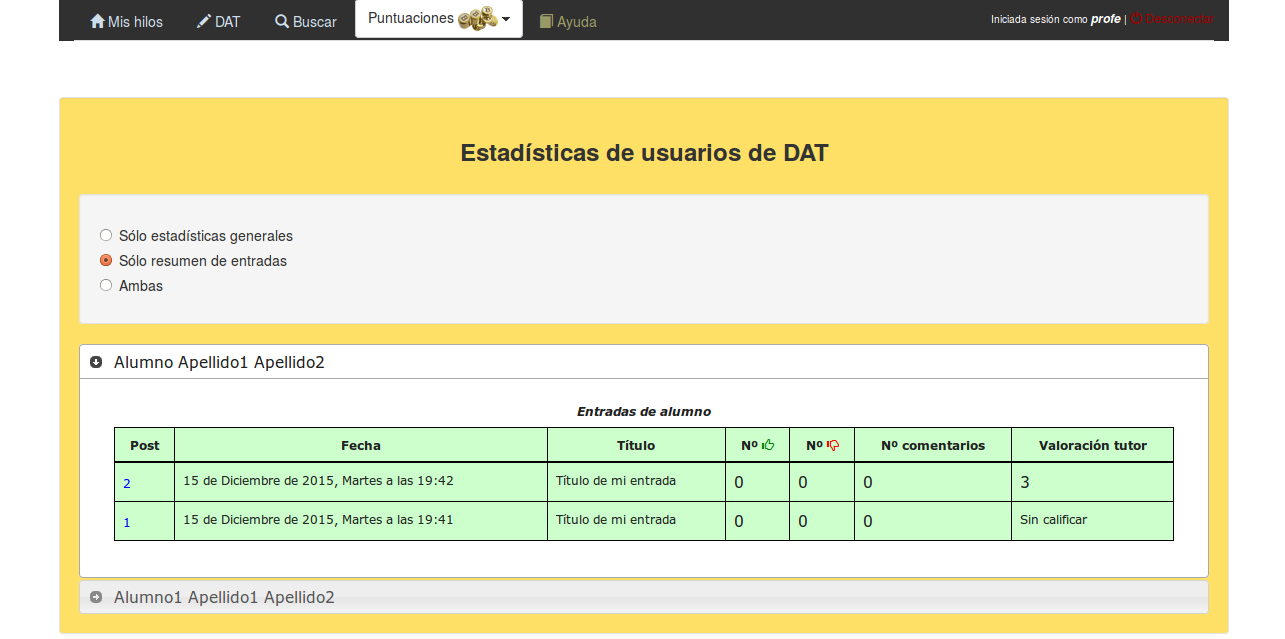
\includegraphics[width=17cm, keepaspectratio]{imagenes/HiloAlumnoEstadisticas}}
  \caption{\textit{P\'agina de ranking.}}
  \label{fig:estadisticas}
\end{figure}


\subsubsection{Informaci\'on de las puntuaciones} 
\label{sec:informacionpuntuaciones}
El documento \textit{HTML} mostrado en la figura~\ref{fig:informacionpuntuaciones} muestra informaci\'on sobre las condiciones o bases de las puntuaciones. 
La p\'agina es servida tras una previa petici\'on \texttt{GET} del cliente mediante el correspondiente recurso \footnote{URL correspondiente a la p\'agina de 
bases de las puntuaciones:\\ \texttt{/planetablogs/tutores/hilo/\textit(IdAsignatura)/infopuntuaciones/}}. La vista asociada a ese recurso es 
\texttt{infopuntuaciones}, la cual devuelve la plantilla \texttt{infopuntuaciones.html} que crea el documento \textit{HTML} de la respuesta.

A esta p\'agina solamente puede acceder un usuario que se haya registrado previamente en la aplicaci\'on.

La cabecera re\'une todos los \'items de la barra de navegaci\'on explicada en la secci\'on~\ref{sec:hilos}.

La vista \texttt{puntuaciones} recibe como par\'ametro el Id del hilo, y mediante ese Id procesa la petici\'on obteniendo el objeto completo de dicha 
asignatura. El contenedor de la plantilla re\'une una serie de condiciones de texto plano mediante una lista num\'erica (etiqueta \texttt{<ol>}) y 
en la parte inferior muestra una tabla \textit{HTML} que resume la consecuci\'on de niveles con respecto a la puntuaci\'on obtenida. Al pasar el rat\'on por encima 
de un nivel, y mediante los eventos \textit{JavaScript}, \texttt{mouseover} y \texttt{mouseout} del fichero \texttt{infopuntuaciones.js}, se a\~nade 
(\textit{.addClass}) y se remueve (\textit{.removeClass}) una clase \textit{CSS} que colorea seg\'un el nivel se\~nalado.

\begin{figure}
  \centering
  \doublebox{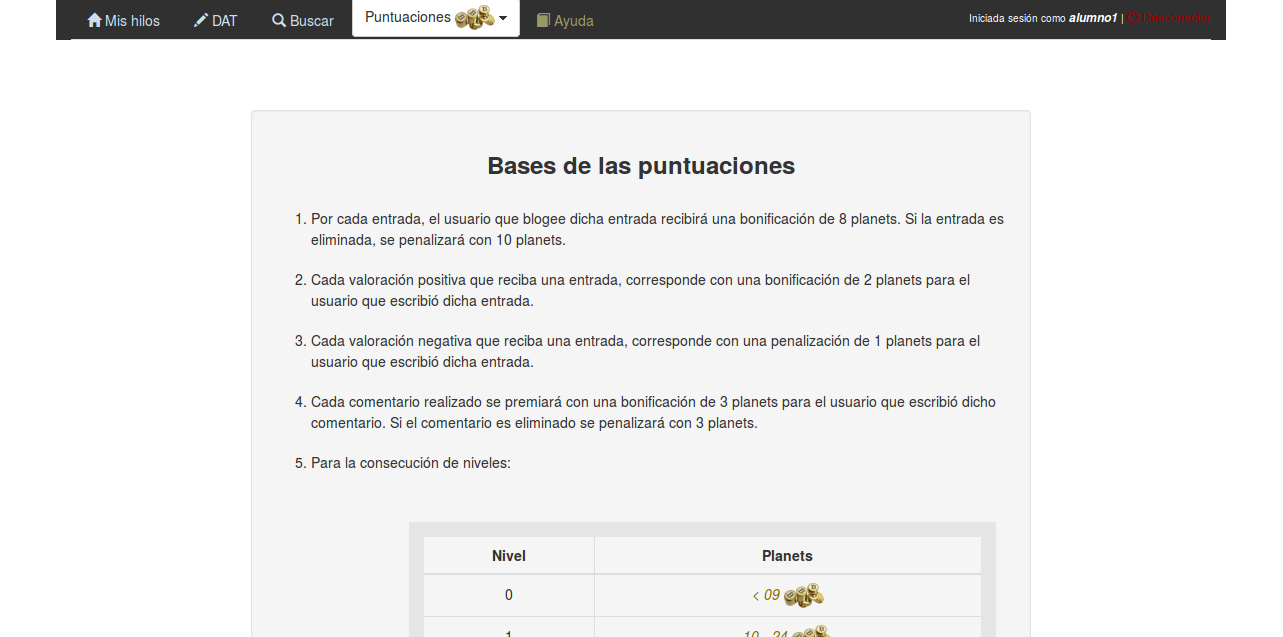
\includegraphics[width=17cm, keepaspectratio]{imagenes/HiloAlumnoInfoPuntuaciones}}
  \caption{\textit{P\'agina con las bases de las puntuaciones.}}
  \label{fig:informacionpuntuaciones}
\end{figure}


\subsubsection{Vistas con AJAX} 
\label{sec:vistasajax}
Hasta ahora hemos visto todas las vistas que procesaban peticiones con necesidad de renderizar una plantilla como respuesta a esas solicitudes. Con 
\textit{AJAX} se han definido numerables vistas para intercambio de datos entre cliente y servidor sin necesidad de recargar la p\'agina, simplemente 
enviando como respuesta el cacho de \textit{HTML} que se necesita.

Las vistas implementadas con \textit{AJAX} en el fichero \texttt{views.py} de este proyecto son las siguientes:

\begin{itemize}
  \item {\bfseries \textit{Eliminar hilo en presentaci\'on de alumno}}: En la secci\'on donde se ubican \textit{Mis hilos}, cada hilo de la lista mostrada 
  tiene dos botones a su derecha. El bot\'on \texttt{Eliminar} mediante el evento \textit{onClick} llama a la funci\'on \textit{JavaScript} 
  \texttt{EliminarHilo} del fichero \texttt{presentacionalum.js}. Esta funci\'on lanza un di\'alogo definido por \textit{BootStrap} que da la opci\'on de
  eliminar el hilo o cancelar dicha acci\'on tal y como se muestra en la figura~\ref{fig:eliminarhiloalumno}. 
  
  Al hacer click sobre el bot\'on \texttt{Eliminar} del cuadro de di\'alogo, se realiza una petici\'on \textit{AJAX} de tipo \texttt{GET} a la vista 
  \texttt{eliminarasignaturaalumno}. La petici\'on es enviada desde el fichero \texttt{presentacionalum.js} usando \textit{jQuery} e incluye como dato el 
  Id de la asignatura. Una vez llega la solicitud al servidor, la vista filtra por medio de ese Id y del Id del alumno en los modelos \texttt{RSS}, 
  \texttt{Valoracion} y \texttt{Entrada}, para realizar un borrado (\texttt{.delete}) de todos los objetos que ofrecen alguna dependencia con el hilo. La 
  funci\'on \textit{AJAX} no recibe ning\'un dato como respuesta.
  
  \begin{figure}
    \centering
    \Ovalbox{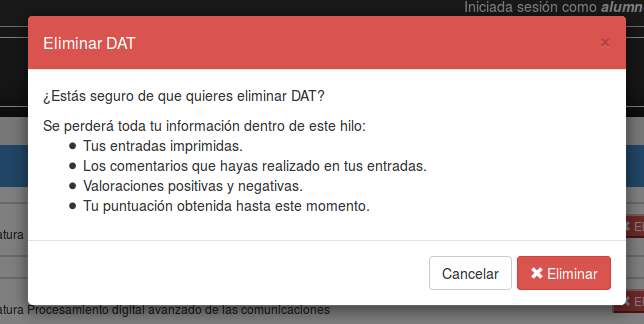
\includegraphics[width=17cm, keepaspectratio]{imagenes/PresentacionAlumnoEliminarHilo}}
    \caption{\textit{Eliminar hilo en una presentaci\'on de alumno.}}
    \label{fig:eliminarhiloalumno}
  \end{figure}

  \item {\bfseries \textit{Agregar hilo en presentaci\'on de tutor}}: En \textit{Hilos disponibles}, cada hilo de la lista ofrece la posibilidad de pinchar 
  sobre un bot\'on \texttt{A\~nadir} de color azul. Mediante el evento \textit{onClick} llama a la funci\'on \textit{JavaScript} \texttt{Agregar} del 
  fichero \texttt{presentacionprof.js}. Esta funci\'on realiza una petici\'on \textit{AJAX} de tipo \texttt{GET} a la vista 
  \texttt{agregarasignaturaprofesor}. La petici\'on es enviada desde el fichero \texttt{presentacionprof.js} usando \textit{jQuery} e incluye como dato el 
  Id de la asignatura. La vista filtra por el par\'ametro recibido en el modelo \texttt{Asignatura}. Una vez consigue el hilo, asocia al usuario que 
  puls\'o el bot\'on a\~nadir a ese hilo. La funci\'on \textit{AJAX} recibe una respuesta con c\'odigo \textit{HTML}. Mediante la funci\'on \textit{jQuery} 
  \texttt{.prepend} en la presentaci\'on se agrega el hilo en \textit{Mis hilos}, mientras que paralelamente con la funci\'on \texttt{.hide} de 
  \textit{jQuery-ui} se elimina de \textit{Hilos disponibles}.

  \item {\bfseries \textit{Eliminar hilo en presentaci\'on de tutor}}: En la secci\'on donde se ubican \textit{Mis hilos}, cada hilo de la lista mostrada 
  tiene dos botones a su derecha. El bot\'on \texttt{Eliminar} mediante el evento \textit{onClick} llama a la funci\'on \textit{JavaScript} 
  \texttt{EliminarHilo} del fichero \texttt{presentacionprof.js}. Esta funci\'on lanza un di\'alogo definido por \textit{BootStrap} que da la opci\'on de
  eliminar el hilo o cancelar dicha acci\'on tal y como se muestra en la figura~\ref{fig:eliminarhilotutor}. 
  
  Al hacer click sobre el bot\'on \texttt{Eliminar} del cuadro de di\'alogo, se realiza una petici\'on \textit{AJAX} de tipo \texttt{GET} a la vista 
  \texttt{eliminarasignaturaprofesor}. La petici\'on es enviada desde el fichero \texttt{presentacionprof.js} usando \textit{jQuery} e incluye como dato el 
  Id de la asignatura. Una vez llega la solicitud al servidor, la vista filtra por medio de ese Id y remueve el objeto con Id del tutor en el modelo
  \texttt{Asignatura} mediante el m\'etodo \textit{.remove}. La funci\'on \textit{AJAX} recibe una respuesta con c\'odigo \textit{HTML}. Mediante la funci\'on 
  \textit{jQuery} \texttt{.prepend} en la presentaci\'on se agrega el hilo en \textit{Hilos disponibles}, mientras que paralelamente con la funci\'on 
  \texttt{.hide} de \textit{jQuery-ui} se elimina de \textit{Mis hilos}.
  
  \begin{figure}
    \centering
    \Ovalbox{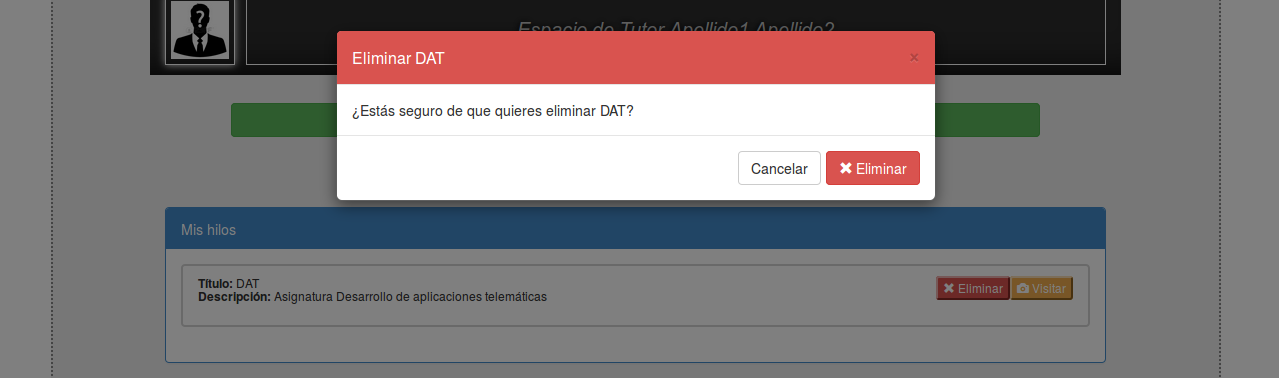
\includegraphics[width=17cm, keepaspectratio]{imagenes/PresentacionTutorEliminarHilo}}
    \caption{\textit{Eliminar hilo en una presentaci\'on de tutor.}}
    \label{fig:eliminarhilotutor}
  \end{figure}
  
  \item {\bfseries \textit{Agregar comentario en hilo de alumno}}: Las entradas de un hilo dan la posibilidad de comentar esa entrada mediante un texto
  introducido en una etiqueta \texttt{<textarea>} y un bot\'on \texttt{Enviar} como se muestra en la figura~\ref{fig:agregarcomentario}.
  
  El bot\'on \texttt{Enviar} mediante el evento \textit{onClick} llama a la funci\'on \textit{JavaScript}\\ \texttt{AgregarComentario} del fichero 
  \texttt{index.js}. Realiza una petici\'on \textit{AJAX} de tipo \texttt{GET} a la vista \texttt{agregarcomentario}. La petici\'on es enviada desde el 
  fichero \texttt{index.js} usando \textit{jQuery} e incluye como datos el Id de la asignatura, el Id de la entrada, el Id del usuario y la descripci\'on.
  Una vez llega la solicitud al servidor, si la descripci\'on es distinto de \textit{null} (es decir, se ha escrito alg\'un comentario), la vista crea un
  objeto \texttt{Comentario} y lo guarda en base de datos. Suma la valoraci\'on del comentario al alumno de la asignatura correspondiente y actualiza su 
  nivel. Por \'ultimo, la vista declara datos a trav\'es de un elemento que incluye dos \textit{JSON} (\texttt{json\_usuario} y \texttt{json\_comentario})
  que se traspasar\'an por medio de la respuesta \texttt{HTTP} al cliente. La funci\'on \textit{AJAX} recibe una respuesta con c\'odigo \textit{HTML} y datos \textit{JSON}. 
  Mediante la funci\'on \textit{jQuery} \texttt{.append} en la plantilla se plasma el comentario en la parte inferior de la entrada.
  
  \begin{figure}
    \centering
    \Ovalbox{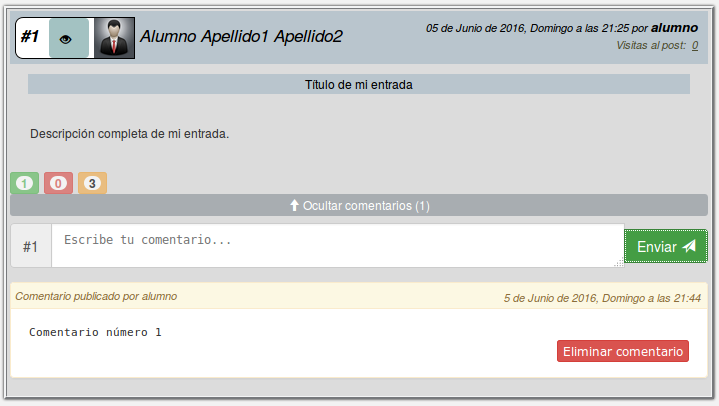
\includegraphics[width=17cm, keepaspectratio]{imagenes/HiloAlumnoEntradaComentario}}
    \caption{\textit{Comentario agregado en una entrada.}}
    \label{fig:agregarcomentario}
  \end{figure}
  
  \item {\bfseries \textit{Eliminar comentario en hilo de alumno o tutor}}: Las entradas de un hilo dan la posibilidad de eliminar comentarios sobre esa 
  entrada al pulsar el bot\'on \texttt{Eliminar comentario} que mediante el evento \textit{onClick} llama a la funci\'on \textit{JavaScript} 
  \texttt{EliminarComentario} del fichero \texttt{index.js}.
  
  La petici\'on \textit{AJAX} de tipo \texttt{GET} se vincula con la vista \texttt{eliminarcomentario}. La solicitud es enviada desde el 
  fichero \texttt{index.js} usando \textit{jQuery} e incluye como datos el Id de la asignatura y el Id del comentario.
  El servidor procesa la solicitud obteniendo el objeto \texttt{Comentario} a borrar. Cuando lo obtiene realiza un borrado con el m\'etodo \textit{.delete} 
  y resta la puntuaci\'on del objeto \texttt{Valoracion} perteneciente al usuario que elimina el comentario y actualiza su nivel.
  La funci\'on \textit{AJAX} recibe una respuesta con c\'odigo \textit{HTML}. Mediante la funci\'on \textit{jQuery} \texttt{.remove} suprime el comentario de la 
  plantilla y con la funci\'on \texttt{.show} muestra un mensaje de informaci\'on de borrado como se ve en la figura~\ref{fig:eliminarcomentario}.
  
  \begin{figure}
    \centering
    \Ovalbox{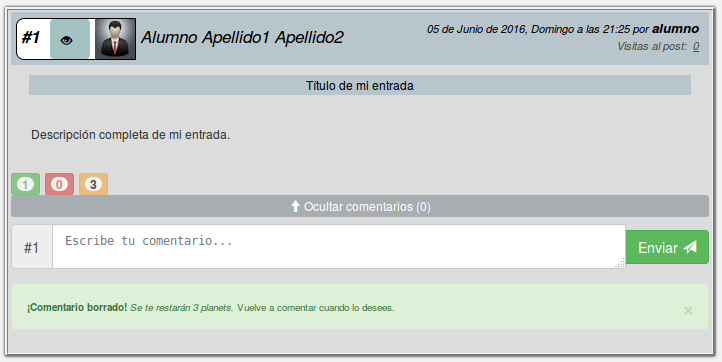
\includegraphics[width=17cm, keepaspectratio]{imagenes/HiloAlumnoEntradaComentarioBorrado}}
    \caption{\textit{Comentario eliminado en una entrada.}}
    \label{fig:eliminarcomentario}
  \end{figure}
  
  \item {\bfseries \textit{Valoraci\'on positiva y negativa de una entrada}}: Dentro de cada entrada se agrupan dos botones, de color verde para 
  valoraciones positivas y de color rojo para valoraciones negativas (figura~\ref{fig:hilos}(a)). Son enlaces \textit{hyperlink} que mediante el evento \textit{onClick} llaman a las 
  funciones \textit{JavaScript} \texttt{Up} o \texttt{Down} respectivamente. Estas funciones se definen en el fichero \texttt{index.js}. 
  
  Ambas funciones env\'ian una petici\'on \textit{AJAX} de tipo \texttt{GET} a su correspondiente vista mediante su recurso o URL. La petici\'on es enviada 
  desde el fichero \texttt{index.js} usando \textit{jQuery} e incluye como datos el Id de la asignatura, el Id del alumno, el Id de la entrada y el entero 
  Up o Down (valor del bot\'on antes de enviar la petici\'on).
  
  La vista \texttt{up} procesar\'a una valoraci\'on positiva. La vista crea un objeto en el modelo \texttt{Up} con los par\'ametros pasados en la solicitud. 
  Guarda el objeto y modifica la entrada del modelo \texttt{Entrada} en la que se efectu\'o el click del bot\'on positivo. En el objeto \texttt{Entrada} se
  cambia el campo \textit{total} (suma dos puntos que es la puntuaci\'on que se bonifica al hacer una valoraci\'on positiva) y el campo \textit{totalup} 
  (indica el total de valoraciones positivas que ha recibido esa entrada). Por \'ultimo, la vista modifica el objeto \texttt{Valoracion} sumando esos dos 
  puntos y actualizando el nivel al usuario.
  
  La vista \texttt{down} procesar\'a una valoraci\'on negativa. La vista crea un objeto en el modelo \texttt{Down} con los par\'ametros pasados en la 
  solicitud. Guarda el objeto y modifica la entrada del modelo \texttt{Entrada} en la que se efectu\'o el click del bot\'on negativo. En el objeto 
  \texttt{Entrada} se cambia el campo \textit{total} (resta un punto que es la puntuaci\'on que se penaliza al hacer una valoraci\'on negativa) y el campo 
  \textit{totaldown} (indica el total de valoraciones negativas que ha recibido esa entrada). Por \'ultimo, la vista modifica el objeto \texttt{Valoracion} 
  restando ese punto y actualizando el nivel al usuario.
  
  La funci\'on \textit{AJAX} recibe una respuesta con c\'odigo \textit{HTML}. Mediante la funci\'on \textit{jQuery} \texttt{.html} en la entrada del documento \textit{HTML} 
  se crean dos botones deshabilitados con la cantidad total de valoraciones positivas y negativas que ha recibido (figura~\ref{fig:hilos}(b))
  
  \begin{figure}
    \centering
    \subfigure[Botones sin valoraci\'on]{\Ovalbox{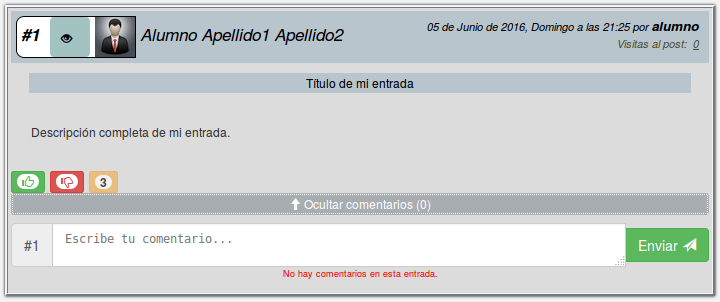
\includegraphics[width=7cm]{imagenes/SinValoracion}}}
    \subfigure[Botones con valoraci\'on]{\Ovalbox{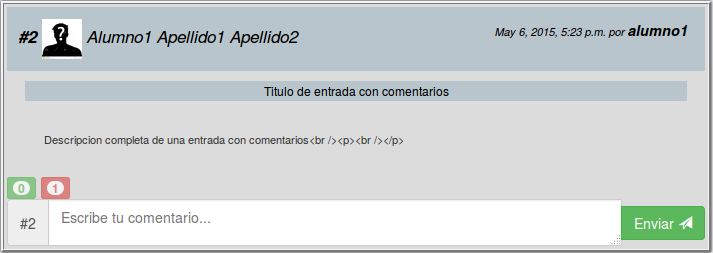
\includegraphics[width=7cm]{imagenes/ConValoracion}}}
    \caption{\textit{Valoraci\'on de una entrada.}}
    \label{fig:hilos}
  \end{figure}

  \item {\bfseries \textit{Eliminar entrada en hilo de tutor}}: Un tutor puede eliminar las entradas de un hilo escritas por un alumno a trav\'es del 
  bot\'on \texttt{Eliminar entrada}, tanto entradas ya valoradas (figura~\ref{fig:eliminarentrada}(a)) como entradas no valoradas 
  (figura~\ref{fig:eliminarentrada}(b)). Al pulsar sobre el bot\'on el evento \textit{onClick} llama a la funci\'on 
  \textit{JavaScript} \texttt{EliminarEntradaPopUp} del fichero \texttt{index\_tutor.js}. Esta funci\'on lanza un di\'alogo definido por \textit{BootStrap} 
  que da la opci\'on de eliminar la entrada o cancelar dicha acci\'on tal y como se muestra en la figura~\ref{fig:eliminarentrada}(c). 
  
  Al hacer click sobre el bot\'on \texttt{Eliminar} del cuadro de di\'alogo, se realiza una petici\'on \textit{AJAX} de tipo \texttt{GET} a la vista 
  \texttt{eliminarentrada}. La petici\'on es enviada desde el fichero \texttt{index\_tutor.js} usando \textit{jQuery} e incluye como datos el 
  Id de la asignatura y el Id de la entrada. La solicitud es aceptada en el servidor. La vista remueve el objeto \texttt{Entrada} mediante el m\'etodo 
  \textit{.remove} y elimina las valoraciones negativas o positivas de los modelos \texttt{Up} y \texttt{Down}. Adem\'as realiza un rec\'alculo del objeto 
  \texttt{Valoracion} al suprimir estas valoraciones y actualiza el nivel del alumno.
  
  La funci\'on \textit{AJAX} no recibe ning\'un dato como respuesta.
  
  \begin{figure}
    \centering
    \subfigure[Entrada en hilo de tutor con valoraci\'on.]{\Ovalbox{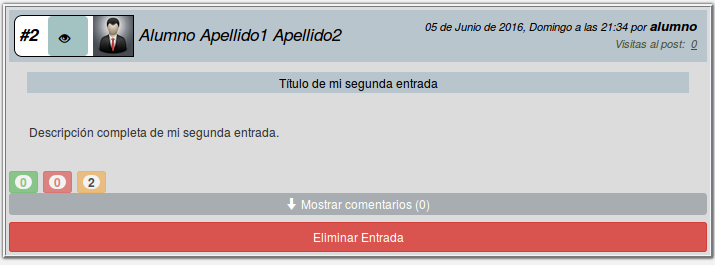
\includegraphics[width=10cm]{imagenes/EntradaTutorConValoracion}}}
    \subfigure[Entrada en hilo de tutor sin valoraci\'on.]{\Ovalbox{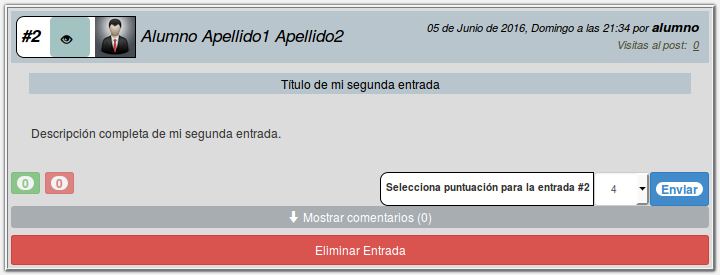
\includegraphics[width=10cm]{imagenes/EntradaTutorSinValoracion}}}
    \subfigure[Cuadro de di\'alogo de borrado.]{\Ovalbox{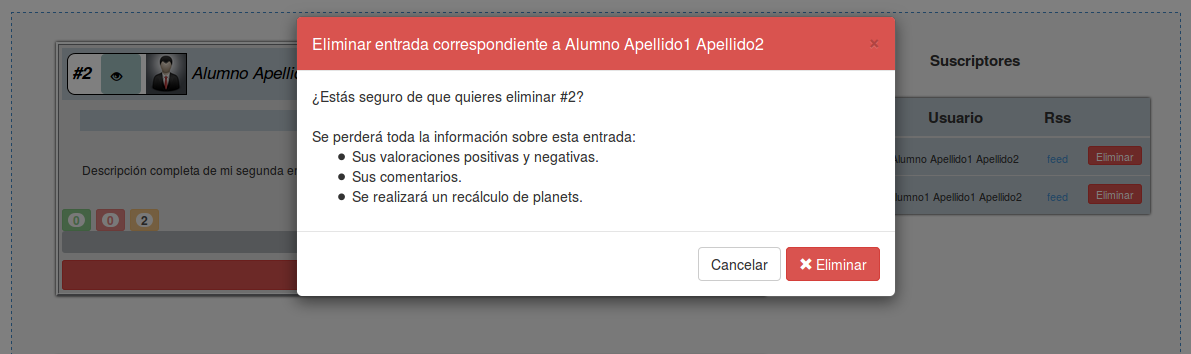
\includegraphics[width=10cm]{imagenes/HiloTutorEliminarEntrada}}}
    \caption{\textit{Eliminaci\'on de una entrada en el hilo de un tutor.}}
    \label{fig:eliminarentrada}
  \end{figure}

  
  \item {\bfseries \textit{Eliminar alumno en hilo de tutor}}: Un tutor puede eliminar los alumnos suscritos a un hilo a trav\'es del 
  bot\'on \texttt{Eliminar} (figura~\ref{fig:eliminaralumno}(a)). Al pulsar sobre el bot\'on el evento \textit{onClick} llama a la funci\'on 
  \textit{JavaScript} \texttt{EliminarAlumnoPopUp} del fichero \texttt{index\_tutor.js}. Esta funci\'on lanza un di\'alogo definido por \textit{BootStrap} 
  que da la opci\'on de eliminar el alumno o cancelar dicha acci\'on tal y como se muestra en la figura~\ref{fig:eliminaralumno}(b). 
  
  Al hacer click sobre el bot\'on \texttt{Eliminar} del cuadro de di\'alogo, se realiza una petici\'on \textit{AJAX} de tipo \texttt{GET} a la vista 
  \texttt{eliminaralumno}. La petici\'on es enviada desde el fichero \texttt{index\_tutor.js} usando \textit{jQuery} e incluye como datos el 
  Id de la asignatura y el Id del alumno. La solicitud es aceptada en el servidor. La vista remueve el objeto \texttt{RSS} mediante el m\'etodo 
  \textit{.delete} y procede a la eliminaci\'on de todas las entradas del alumno en ese hilo. Adem\'as se elimina su objeto \texttt{Valoracion},
  por lo que se habr\'a realizado un borrado completo de ese alumno en ese hilo.
  
  La funci\'on \textit{AJAX} no recibe ning\'un dato como respuesta.
  
  \begin{figure}
    \centering
    \subfigure[Tabla de suscriptores en hilo de tutor.]{\Ovalbox{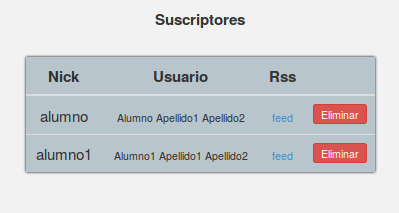
\includegraphics[width=8cm]{imagenes/HiloTutorAlumnos}}}
    \subfigure[Cuadro de di\'alogo de borrado.]{\Ovalbox{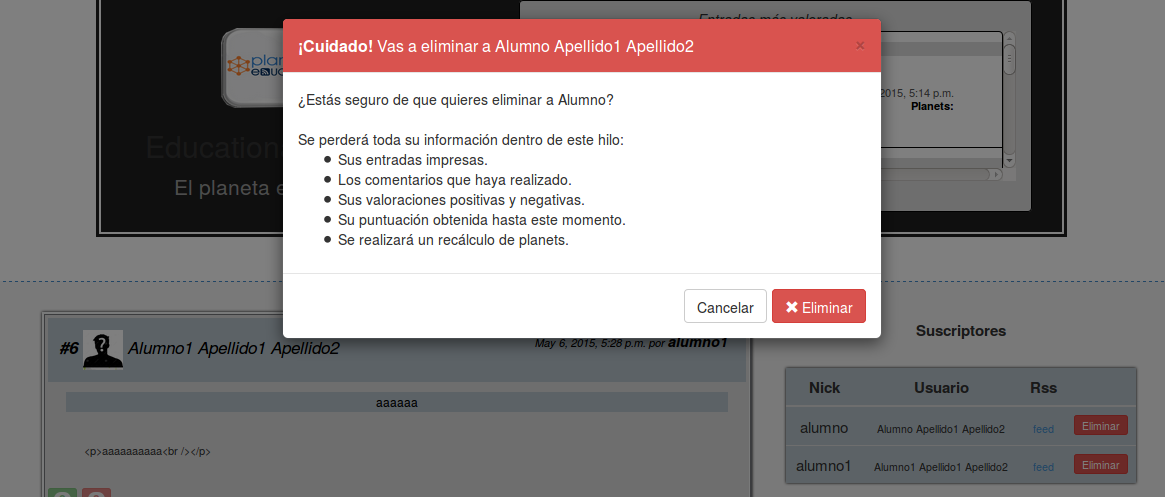
\includegraphics[width=8cm]{imagenes/HiloTutorEliminarAlumno}}}
    \caption{\textit{Eliminaci\'on de un alumno en el hilo de un tutor.}}
    \label{fig:eliminaralumno}
  \end{figure}
  
  
  \item {\bfseries \textit{B\'usqueda avanzada}}: Un alumno o un tutor tienen la opci\'on de buscar entradas por \textit{Nick de usuario} o 
  \textit{Id de entrada}. Cada opci\'on se selecciona con una etiqueta \texttt{<select>}. Al pulsar sobre el bot\'on \texttt{Buscar} el evento 
  \textit{onClick} llama a la funci\'on \textit{JavaScript} \texttt{Buscar} del fichero \texttt{buscar.js}. 
  
  Ambas acciones ejecutan una petici\'on \textit{AJAX} de tipo \texttt{GET}. La petici\'on es enviada desde el fichero \texttt{buscar.js} usando 
  \textit{jQuery} e incluye como datos el Id de la opci\'on y el texto escrito.

  En la figura~\ref{fig:buscarajax}(a) se procede a buscar por \textit{Nick de usuario}. La solicitud \textit{AJAX} vincula su recurso \textit{URL} a la 
  vista \texttt{buscarNickUsuario}. Comprueba que el texto enviado en la petici\'on no est\'a vac\'io y si existe un \texttt{username} que coincide con lo
  introducido. Una vez validado correctamente se crean dos listas \textit{JSON} de usuario (\texttt{list\_usuario}) y de entradas (\texttt{list\_entradas}) 
  filtradas por el Id del alumno. Estos datos \textit{JSON} son inclu\'idas como respuesta \texttt{HTTP} al cliente. En caso de que la validaci\'on sea incorrecta 
  se enviar\'a como respuesta \texttt{HTTP} un \textit{JSON} vac\'io que saltar\'a en la plantilla renderizada como un mensaje de aviso.

  En la figura~\ref{fig:buscarajax}(b) se procede a buscar por \textit{Id de entrada}. La solicitud \textit{AJAX} vincula su recurso \textit{URL} a la 
  vista \texttt{buscarIdEntrada}. Comprueba que el texto enviado en la petici\'on no est\'a vac\'io y si existe un Id de entrada que coincide con lo
  introducido. Una vez validado correctamente se crean dos listas \textit{JSON} de usuario (\texttt{list\_usuario}) y de entrada (\texttt{list\_entrada}). 
  Estos datos \textit{JSON} son inclu\'idas como respuesta \texttt{HTTP} al cliente. En caso de que la validaci\'on sea incorrecta se enviar\'a como respuesta \texttt{HTTP} 
  un \textit{JSON} vac\'io que saltar\'a en la plantilla renderizada como un mensaje de aviso.
  
  La funci\'on \textit{AJAX} recibe una respuesta con c\'odigo \textit{HTML}. Mediante la funci\'on \textit{jQuery} \texttt{.append} en el contenedor del documento 
  \textit{HTML} se agrega las entradas enviadas en la respuesta \texttt{HTTP}.
  
  \begin{figure}
    \centering
    \subfigure[Buscar entradas por Nick de usuario.]{\Ovalbox{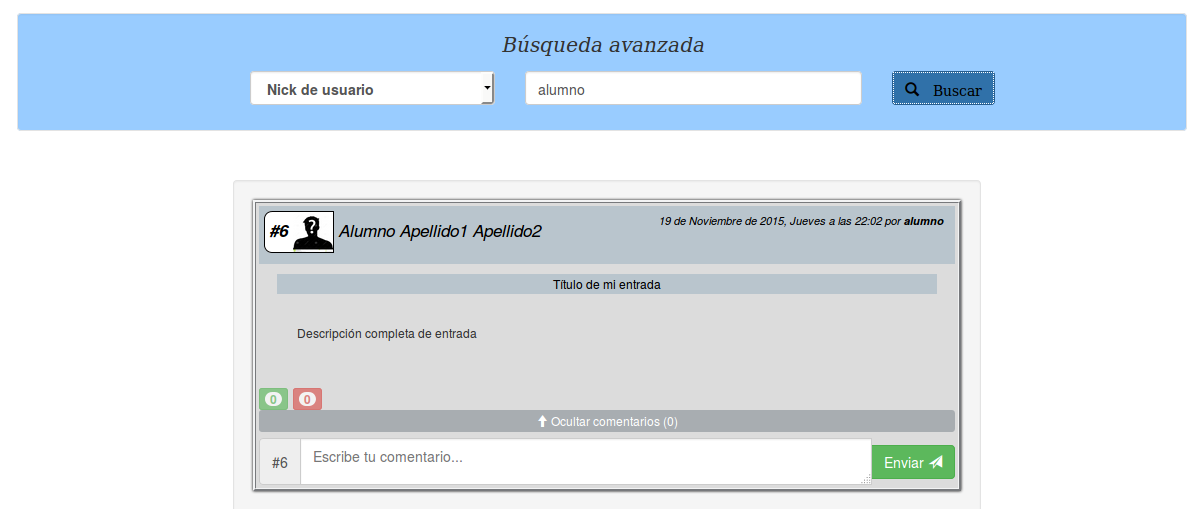
\includegraphics[width=10cm]{imagenes/HiloAlumnoBuscarPorNick}}}
    \subfigure[Buscar entrada por Id de entrada.]{\Ovalbox{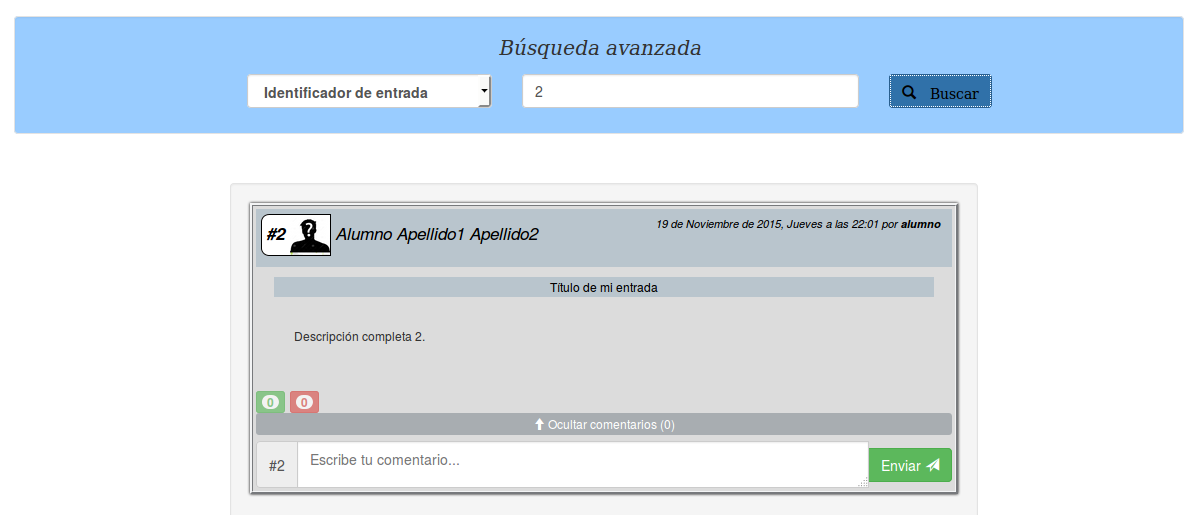
\includegraphics[width=10cm]{imagenes/HiloAlumnoBuscarPorId}}}
    \caption{\textit{Ejecuci\'on de una b\'usqueda.}}
    \label{fig:buscarajax}
  \end{figure}
  
\end{itemize}





\subsubsection{Cierre de sesi\'on} 
\label{sec:cierresesion}
El enlace mostrado en la figura~\ref{fig:cierresesion} en color rojo (\textit{Desconectar}) corresponde con el cierre de sesi\'on por parte de alumno o 
tutor. Al pulsar sobre el enlace se produce una petici\'on \texttt{GET} del cliente. La vista asociada al recurso interno del enlace es \texttt{salir}, la cual 
redirecciona a la plantilla \texttt{inicio.html} que crea el documento \textit{HTML} de la respuesta.

Este enlace se sit\'ua en la parte derecha de la barra de navegaci\'on de cualquier plantilla dentro de la aplicaci\'on que se cargue despu\'es de un previo
registro.
\begin{figure}
  \centering
  \Ovalbox{
\includegraphics[width=10cm, keepaspectratio]{imagenes/CierreSesion}}
  \caption{\textit{Enlace de cierre de sesi\'on.}}
  \label{fig:cierresesion}
\end{figure}


%%%%%%%%%%%%%%%%%%%%%%%%%%%%%%%%%%%%%%%%%%%%%%%%%%%%%%%%%%%%%%%%%%%%%%%%%%%%%%%%
%%%%%%%%%%%%%%%%%%%%%%%%%%%%%%%%%%%%%%%%%%%%%%%%%%%%%%%%%%%%%%%%%%%%%%%%%%%%%%%%
% RESULTADOS %
%%%%%%%%%%%%%%%%%%%%%%%%%%%%%%%%%%%%%%%%%%%%%%%%%%%%%%%%%%%%%%%%%%%%%%%%%%%%%%%%

\cleardoublepage
\chapter{Prueba en entorno real}
\label{chap:prueba}
En las secciones de este cap\'itulo se va a detallar todo lo involucrado en la prueba de la aplicaci\'on web que se realiz\'o en un entorno real. Este 
entorno se situa en una clase de $2^\circ$ de Ciclos Formativos de Grado Superior de Administraci\'on de Sistemas Inform\'aticos y Redes. Los usuarios 
comprometidos son el tutor, Don Jos\'e Ignacio Huertas, y los doce alumnos que conformaban la clase.

\section{Preparaci\'on de la prueba}
\label{seccion:preparacionprueba}
Antes de emprender con la prueba, se organiz\'o un proceso para asignar dicha prueba a un tutor que estuviera dispuesto a promoverla.

A trav\'es del profesor, Don Gregorio Robles Mart\'inez y la colaboraci\'on de Don Jes\'us Moreno, se lleg\'o a un acuerdo con Don Jos\'e 
Ignacio Huertas, profesor de $2^\circ$ de Ciclos Formativos de Grado Superior de Administraci\'on de Sistemas Inform\'aticos y Redes:

\begin{shaded}
\noindent\textbf{\textsf{
From: Jes\'us Moreno\\
To: Jos\'e Ignacio Huertas, Gregorio Robles, Adri\'an S\'aez\\
Fecha: 19 de octubre de 2015\\
}}
\emph{
Hola, Adri\'an,\\
He hablado con Jos\'e Ignacio Huertas, que est\'a en copia, sobre la nueva implementaci\'on del planeta de blogs que has realizado y la ha 
encantado la idea. \\
Jos\'e Ignacio da clases en un ciclo superior de inform\'atica y promueve el uso de los blogs entre sus alumnos. Adem\'as ya conoc\'ia la 
antigua versi\'on del planeta, FAVS, que ya us\'o con sus estudiantes hace unos a\~nos, as\'i que est\'a con ganas de probar esta nueva 
implementaci\'on de la herramienta.\\
Si os parece, os dejo para que pod\'ais acordar c\'omo comenzar con las pruebas.\\
Saludos!
}
\end{shaded}

\begin{shaded}
\noindent\textbf{\textsf{
From: Gregorio Robles\\
To: Jos\'e Ignacio Huertas, Jes\'us Moreno, Adri\'an S\'aez\\
Fecha: 19 de octubre de 2015\\
}}
\emph{
Gracias, Jes\'us. !`Y estupendo poder contar contigo Jos\'e Ignacio!\\
Adri\'an, ?`cu\'ando crees que estar\'ia listo todo para probarlo?\\
saludos, Gregorio
}
\end{shaded}

\begin{shaded}
\noindent\textbf{\textsf{
From: Adri\'an S\'aez\\
To: Jos\'e Ignacio Huertas, Jes\'us Moreno, Gregorio Robles\\
Fecha: 20 de octubre de 2015\\
}}
\emph{
Buenos d\'ias,\\
antes de nada, much\'simas gracias a todos por promover el nuevo planeta de blogs y que se pueda probar en un entorno real antes de su defensa.\\
Respecto a la fecha que estar\'ia listo, ahora estoy trabajando duro para arreglar unas cosillas y calculo que a mediados de la semana que viene estar\'a listo para 
ultimar detalles y poder probarlo, ?`Qu\'e os parece?\\
Un saludo, Adri\'an.
}
\end{shaded}

\begin{shaded}
\noindent\textbf{\textsf{
From: Jos\'e Ignacio Huertas\\
To: Gregorio Robles, Jes\'us Moreno, Adri\'an S\'aez\\
Fecha: 21 de octubre de 2015\\
}}
\emph{
Hola Adri\'an,\\
un placer conocerte y tener la oportunidad de usar la nueva versi\'on del planeta de blogs.\\
Espero tus noticias.\\
Un saludo,\\
JI
}\newline
\end{shaded}

\subsection{Pasos iniciales}
\label{subseccion:correosypasos}

\texttt{Primer paso}: Se facilit\'o un tutorial para tutor y alumnos, en \'el se indicaban unos pasos iniciales a seguir para el correcto uso de la aplicaci\'on. Estos 
pasos fueron los siguientes:
\begin{itemize}
	\item Pasos iniciales del tutor:
	\begin{enumerate}
		\item \textit{URL}: Para comenzar a usar la aplicaci\'on, pegar en el navegador: \\
		\href{http://tfg-asaez.libresoft.es:8080/planetablogs/login/}{http://tfg-asaez.libresoft.es:8080/planetablogs/login/}
		\item \textit{Crear perfil de tutor}: Pulsar sobre el bot\'on verde TUTOR, rellenar todos los campos del formulario (inclu\'ida foto), guardar e 
		identificarse en la p\'agina de inicio.
		\item \textit{Presentaci\'on de tutor}: Es el perfil de cada usuario. S\'olo el usuario registrado como tutor podr\'a crear hilos. Una vez creado, hay 
		que a\~nadirlo a ``Mis hilos'' (solamente puede agregar el hilo a ``Mis hilos'' el tutor que lo crea).
		\item \textit{Dentro del hilo}: La primera vez que se visite el hilo estar\'a vac\'io. Cuando los alumnos se registren y se animen a escribir entradas 
		en el blog asociado al hilo, se mostrar\'an dichas entradas. El tutor har\'a un papel de observador aunque tendr\'a el poder de eliminar entradas, 
		comentarios y alumnos. Con las correspondientes penalizaciones que sufrir\'an los alumnos y que est\'an escritas en la pesta\~na 
		Puntuaciones/Informaci\'on.
		\item \textit{Ayuda}: En la pesta\~na Ayuda en el interior de cada hilo, se mostrar\'a tanto informaci\'on general como consejos de uso, y una secci\'on 
		de sugerencias.
		\item \textit{Buscar}: En la pesta\~na Buscar se podr\'a realizar una b\'usqueda avanzada por nick de usuario o por Id de entrada. En las entradas que se 
		muestren, el tutor podr\'a borrar los comentarios que desee pero no eliminar entradas.\\
	\end{enumerate}
	\item Pasos iniciales del alumno:
	\begin{enumerate}
		\item \textit{URL}: Para comenzar a usar la aplicaci\'on, pegar en el navegador: \\
		\href{http://tfg-asaez.libresoft.es:8080/planetablogs/login/}{http://tfg-asaez.libresoft.es:8080/planetablogs/login/}
		\item \textit{Crear perfil de alumno}: Pulsar sobre el bot\'on verde ALUMNO, rellenar todos los campos del formulario (incluida foto), guardar e 
		identificarse en la p\'agina de inicio.
		\item \textit{Presentaci\'on de alumno}: Es el perfil de cada usuario. El alumno se encontrar\'a con los hilos previamente creados por el tutor. Para que 
		un usuario se suscriba a un hilo, debe introducir en su correspondiente formulario el RSS de su blog.
		\item \textit{Dentro del hilo}: La primera vez que se visite el hilo estar\'a vac\'io. Cuando los alumnos se registren y se animen a escribir entradas en 
		el blog asociado al hilo, se mostrar\'an dichas entradas. El alumno tendr\'a la opci\'on de interactuar comentando y valorando entradas de cualquiera de 
		los alumnos suscritos al hilo. El alumno podr\'a comentar las veces que desee pero s\'olo podr\'a borrar comentarios escritos por el mismo. Y por 
		\'ultimo, s\'olo podr\'a valorar una vez por entrada (Un positivo o un negativo).
		\item \textit{Ayuda}: En la pesta\~na Ayuda en el interior de cada hilo, se mostrar\'a tanto informaci\'on general como consejos de uso, y una secci\'on 
		de sugerencias.
		\item \textit{Buscar}: En la pesta\~na Buscar se podr\'a realizar una b\'usqueda avanzada por nick de usuario o por Id de entrada. En las entradas que 
		se muestren, el alumno podr\'a escribir los comentarios que desee pero s\'olo podr\'a borrarlos si no recarga la p\'agina una vez hecha la b\'usqueda. 
		No tiene la opci\'on de valorar entradas.
	\end{enumerate}
\end{itemize}

\texttt{Segundo paso}: Fue la creaci\'on del hilo por parte del tutor. En este caso, Don Jos\'e Ignacio Huertas asoci\'o el nombre de ``$2^\circ$ ASIR'' a su hilo 
(Figura~\ref{figura:pasohilo}).\\
\begin{figure}[htbp] 
  \centering
  \doublebox{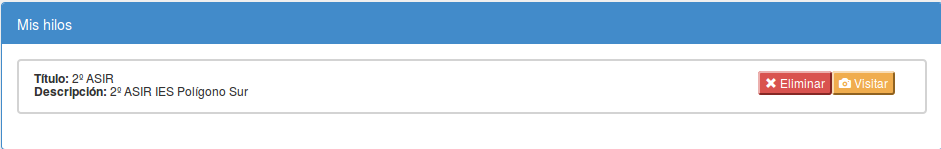
\includegraphics[width=17cm, keepaspectratio]{ImagenesPrueba/Hilo}}
  \caption{Hilo de la prueba.}
  \label{figura:pasohilo}
\end{figure}
Una vez fundado el hilo, se crearon doce perfiles correspondientes a los doce alumnos de la clase, adem\'as de un perfil de administrador que fue manejado 
por Adri\'an S\'aez. Los doce alumnos se suscribieron al hilo introduciendo el RSS de su blog personal de blogdiario.com 
(Figura~\ref{figura:suscriptoreshilo}).
\begin{figure}[htbp] 
  \centering
  \doublebox{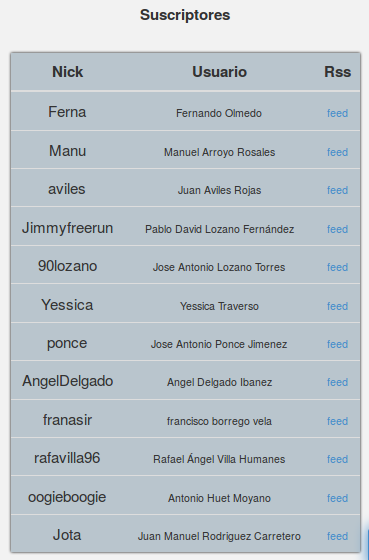
\includegraphics[width=8cm, keepaspectratio]{ImagenesPrueba/Suscriptores}}
  \caption{Suscriptores de la prueba.}
  \label{figura:suscriptoreshilo}
\end{figure}

\texttt{Tercer paso}: Comienzo de uso del planeta. El administrador escribi\'o una entrada en su blog con un mensaje de bienvenida para informar a los usuarios sobre la 
funci\'on de administrador, cooperador en la resoluci\'on de dudas y problemas, y encargado de dar soporte.

Por \'ultimo, los alumnos comenzaron a escribir sus post en sus blogs y una vez plasmados en el planeta, interactuaron con los dem\'as usuarios mediante las funciones 
que dispone la aplicaci\'on. La tem\'atica hablada en el hilo fue de seguridad inform\'atica y administraci\'on de servidores.


\subsection{Archivo \textit{nohup.out}}
\label{subseccion:archivonohup}
El servidor Django de la prueba se lanz\'o con el comando ``nohup''. Este comando permite mantener en ejecuci\'on un comando, pese a salir del terminal, ya que hace que 
se ejecute de forma independiente a la sesi\'on, en segundo plano.

La salida por defecto que saldr\'ia en el terminal, ser\'a procesada a un fichero llamado \texttt{nohup.out} gracias a la ejecuci\'on de dicho comando. Este fichero 
aparecer\'a en la ruta donde nos encontremos ejecutando el programa. 


\subsection{Control estad\'istico}
\label{subseccion:controlestadistico}
Dentro del c\'odigo del proyecto, en el fichero \texttt{views.py}, cada vista se encarga de gestionar y realizar una acci\'on pero adem\'as incluye una l\'inea 
informativa que saca por la salida est\'andar (fichero \texttt{nohup.out}).

Las l\'ineas informativas de todas las vistas siguen el siguiente protocolo:
    {\footnotesize\begin{verbatim}
    [**INICIALESACCION**] Descripci\'on de la funci\'on de la vista.
    \end{verbatim}}

donde INICIALESACCION son letras que identifican la funci\'on de dicha vista, por ejemplo:
    {\footnotesize\begin{verbatim}
    [**AI**] Alumno Identificado en la aplicaci\'on como Pepe.
    \end{verbatim}}
En base al contenido del fichero \texttt{nohup.out} se implement\'o un script para llevar un control estad\'istico de las acciones que realizaron los alumnos durante el 
periodo que dur\'o la prueba. Este script se encarga de parsear el archivo \texttt{nohup.out}. Este fichero se compone de multitud de l\'ineas con la nomenclatura indicada
anteriormente. Cada una de estas l\'ineas se parsea, sacando la informaci\'on necesaria (acci\'on, usuario y/o entrada) y se guarda en una lista. A trav\'es de esta 
lista se crean contadores para cada acci\'on, tanto para las estad\'isticas individuales (se necesitaba la acci\'on y el usuario) como para las estad\'isticas generales 
(se necesita la acci\'on \'unicamente). 

Gracias a este script se pudo contabilizar el n\'umero de veces que cada usuario acced\'ia a una pesta\~na o ejecutaba una operaci\'on de la aplicaci\'on.


\section{Resultados de la prueba}
\label{seccion:preparacionprueba}
A continuaci\'on se hace una valoraci\'on de los resultados obtenidos en la prueba realizada con el fin de estudiar y comprobar el funcionamiento de la 
aplicaci\'on en un entorno real.

\begin{itemize}
	\item \textit{Conclusiones de la clase}: Durante el uso de la prueba surgieron una serie de problemas que se solucionaron sobre la marcha, haciendo 
	efectiva la funci\'on del administrador de proporcionar apoyo y soporte. El tutor facilit\'o la siguiente lista y el administrador propuso e 
	implement\'o una soluci\'on para cada punto:
	\begin{enumerate}
		\item Una alumna se olvid\'o de la contrase\~na y no ha podido recuperarla (no hemos visto la opci\'on). La opci\'on restablecer 
		contrase\~na ser\'ia necesaria.\\
		\texttt{SOLUCI\'ON}: Se ha creado una pesta\~na en el perfil del tutor. El alumno que haya olvidado la contrase\~na puede introducir 
		su nick de usuario y su nueva contrase\~na.
		\item Podr\'ia existir alg\'un mecanismo que controle a aquellos que penalizan al resto y no reciben votos positivos de nadie. Quiz\'as 
		se podr\'ia limitar el n\'umero de ``Me gusta'' y ``No me gusta'' de alguna forma. Por ejemplo, para poder marcar alguna entrada con un 
		``no me gusta'' debes haber recibido un n\'umero de ``me gusta'' antes. O incluso limitarlo a un n\'umero m\'aximo semanal. En cualquier 
		caso, sacar una estad\'istica de esto y que se pueda visualizar por todos ser\'ia bueno: 
		Participante  --  Entradas blog -- $N^\circ$ me gusta (recibidos y dados) -- $N^\circ$ no me gusta (recibidos y dados) -- Comentarios 
		(recibidos y dados)\\
		\texttt{SOLUCI\'ON}: Dentro de cada hilo, en la secci\'on de puntuaciones, se ha a\~nadido otra pesta\~na de estad\'isticas en la que se 
		podr\'a ver estad\'isticas generales con lo recomendado [Participante  --  Entradas blog -- $N^\circ$ me gusta (recibidos y dados) -- 
		$N^\circ$ no me gusta (recibidos y dados) -- Comentarios (recibidos y dados)].
		Tambi\'en se muestra un resumen de las entradas de cada uno de los alumnos.
		Respecto al mecanismo de penalizaci\'on o limitaci\'on de ``Me gusta'', se pensar\'a para futuras implementaciones.
		\item Veo que el tutor solo puede eliminar mensajes o entradas (y penaliza al hacerlo, quitando puntos). En algunas ocasiones podr\'ia ser 
		bueno que el tutor tambi\'en pueda intervenir, de forma que un ``me gusta'' pueda dar puntos (no tengo claro si puntuando igual que si fuera 
		un alumno o algo m\'as).\\
		\texttt{SOLUCI\'ON}: En la parte del tutor, en cada entrada se ha agregado un puntuador con distintas opciones/valores de puntuaci\'on para 
		evaluar a los alumnos en cada entrada [-2, -1, 1, 2, 3 \'o 4 planets]. Son puntuaciones con m\'as poder que los simples 
		``Me gusta/No me gusta'' de los alumnos, ya que puede restar m\'as que un ``No me gusta'' y sumar m\'as que un ``Me gusta''.
		\item En los post que se muestran no se ven v\'ideos o im\'agenes. Esto ha supuesto para mis alumnos un inconveniente grave, dado que eran 
		necesarias para entender algunos posts. Al final se han dado cuenta de que al dar en el nombre se abre el post en el blog correspondiente.\\
		\texttt{SOLUCI\'ON}: Se identificaron las etiquetas de imagen y v\'ideo para el parseo correcto de la descripci\'on de las entradas. Ya se 
		muestran im\'agenes y v\'ideos en las descripciones plasmadas en el planeta.
		\item El cuadro de ``Entradas m\'as valoradas'' me parece muy interesante, aunque no me sale enlazada para que pueda abrirlas directamente 
		al hacer clic en ellas.\\
		\texttt{SOLUCI\'ON}: La secci\'on de ``Entradas m\'as valoradas'' ha sido modificada con links para que se pueda clicar sobre cada entrada 
		y te redirija al post del blog personal.
		\item Quiz\'as ser\'ia interesante, dentro de un hilo, poder crear distintas actividades. Por ejemplo, en mi hilo de $2^\circ$ ASIR se me 
		ocurre que podr\'ia existir una actividad en la que todos tuvieran que escribir una \'unica entrada en el blog referida a alg\'un tema 
		concreto y tener un ranking solo de esa actividad.\\
		\texttt{SOLUCI\'ON}: No se plante\'o ninguna soluci\'on. No obstante, se tuvo en cuenta para futuros trabajos.\\\\
	\end{enumerate}

	\item \textit{Resultados del control estad\'istico}: El script extrajo los siguientes resultados estad\'isticos:
	\begin{enumerate}
		\item En la figura~\ref{figura:estadgener} se muestra los resultados de estad\'isticas generales sobre las acciones totales que se 
		efectuaron.
		\begin{figure}[htbp] 
		  \centering
		  \doublebox{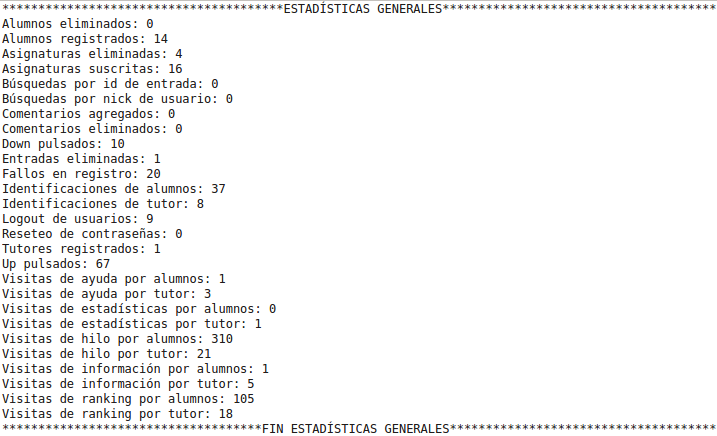
\includegraphics[width=8cm, keepaspectratio]{ImagenesPrueba/EstadGener}}
		  \caption{Estad\'isticas generales de la prueba.}
		  \label{figura:estadgener}
		\end{figure}
		\item En la figura~\ref{figura:estadindiv} se puede visualizar los resultados de estad\'isticas individuales de dos de los doce usuarios 
		suscritos al hilo (por simplicidad).
		\begin{figure}[htbp] 
		  \centering
		  \doublebox{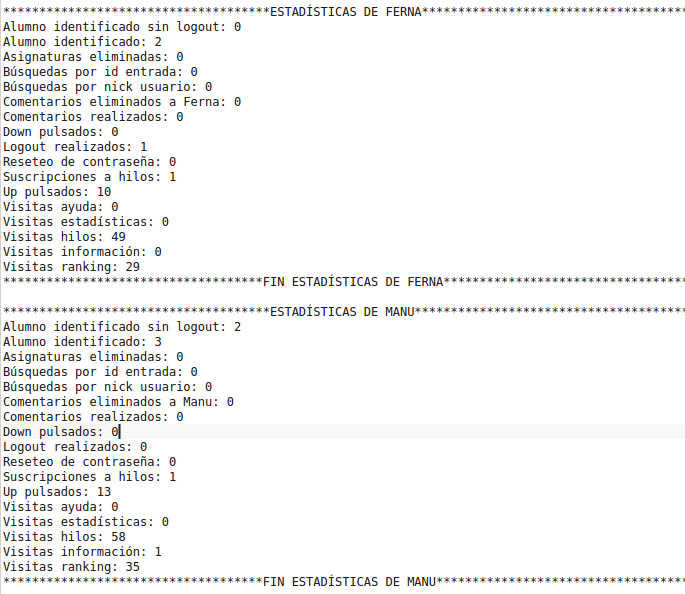
\includegraphics[width=8cm, keepaspectratio]{ImagenesPrueba/EstadIndiv}}
		  \caption{Estad\'isticas individuales de dos usuarios de la prueba.}
		  \label{figura:estadindiv}
		\end{figure}
	\end{enumerate}
\end{itemize}









%%%%%%%%%%%%%%%%%%%%%%%%%%%%%%%%%%%%%%%%%%%%%%%%%%%%%%%%%%%%%%%%%%%%%%%%%%%%%%%%
%%%%%%%%%%%%%%%%%%%%%%%%%%%%%%%%%%%%%%%%%%%%%%%%%%%%%%%%%%%%%%%%%%%%%%%%%%%%%%%%
% CONCLUSIONES %
%%%%%%%%%%%%%%%%%%%%%%%%%%%%%%%%%%%%%%%%%%%%%%%%%%%%%%%%%%%%%%%%%%%%%%%%%%%%%%%%

\cleardoublepage
\chapter{Conclusiones}
\label{chap:conclusiones}
Este cap\'itulo recoger\'a las conclusiones m\'as destacadas, la consecuci\'on de los distintos objetivos marcados previamente a la realizaci\'on del proyecto, las tecnolog\'ias y 
conocimientos adquiridos durante la carrera que han significado un aporte en la realizaci\'on de la aplicaci\'on web, la lecci\'on de lo aprendido en su implementaci\'on 
y una lista de puntos a mejorar o a\~nadir al resultado final del trabajo.

\section{Consecuci\'on de objetivos}
\label{sec:consecucion-objetivos}
\begin{itemize}
  \item \textit {Usabilidad sencilla:} La aplicaci\'on cuenta con botones con una etiqueta totalmente descriptiva, al 
  igual que los enlaces muestran t\'itulos emergentes descriptivos, todo ello para facilitar su usabilidad. Adem\'as se cuenta con dos 
  secciones de ayuda e informaci\'on de uso. El resultado es una aplicaci\'on bastante sencilla de usar. El \'unico punto m\'as complicado se puede dar a la hora de 
  ingresar el \textit{RSS} en un determinado hilo disponible.
  \item \textit {Integraci\'on de elementos sociales:} Objetivo logrado gracias a la secci\'on de escribir comentarios en cada una de las entradas, la puntuaci\'on del tutor, los 
  botones ``Me gusta'' y ``No me gusta'', el elemento popup con la informaci\'on de cada usuario (foto, nombre y apellidos, correo, puntos y nivel),..
  \item \textit {Inclusi\'on de gamificaci\'on:} En la pesta\~na ``Informaci\'on de puntuaciones'' se muestran todas las bases para la obtenci\'on de premio o 
  penalizaci\'on de \textit{planets}, en resumen:\\
  -El usuario que blogee una entrada recibir\'a una bonificaci\'on de 8 \textit{planets}. Si la entrada es eliminada, se penalizar\'a con 10 \textit{planets}.\\
  -Cada valoraci\'on positiva que reciba una entrada corresponde con una bonificaci\'on de 2 \textit{planets} para el usuario que escribi\'o dicha entrada. Cada valoraci\'on 
  negativa corresponde con una penalizaci\'on de 1 \textit{planets}.\\
  -Cada comentario realizado se premiar\'a con una bonificaci\'on de 3 \textit{planets} para el usuario que escribi\'o dicho comentario. Si el comentario es eliminado se 
  penalizar\'a con 3 \textit{planets}.\\
  -La puntuaci\'on del tutor premiar\'a o penalizar\'a al usuario de una entrada con la misma cantidad que valore el tutor en dicha entrada.\\
  -Tabla para la consecuci\'on de niveles.\\
  \item \textit {Adaptabilidad:} Este objetivo ha sido logrado en cualquier navegador y a cualquier anchura de pantalla en port\'atiles u ordenadores de mesa. 
  La adaptabilidad en dispositivos m\'oviles tiene problemas con solapamiento de distintos elementos, como botones, enlaces o el men\'u.
  \item \textit {Dinamismo y rapidez:} \textit{AJAX}, \textit{jQuery} y \textit{jQuery-ui} han logrado este objetivo. Sin necesidad de recargar la p\'agina y con la ayuda 
  de \textit{jQuery}, la aplicaci\'on es capaz de:\\
  -Eliminar hilos, entradas y alumnos.\\
  -Agregar hilos disponibles a ``Mis hilos''.\\
  -Mostrar popup con informaci\'on de usuario y popup con informaci\'on del creador del hilo.\\
  -Mostrar comentarios y ocultarlos.\\
  -Pulsar ``Me gusta'' y ``No me gusta''\\
  -Escribir comentarios y saltar popup con informaci\'on de ganancia de 3 \textit{planets}.\\
  -Zoom en fotos de usuarios.\\
  -B\'usqueda de entradas por id de entrada o por nick de usuario.\\
  Con la ayuda de \textit{jQuery-ui} se ha creado un acorde\'on que ha hecho de la secci\'on de estad\'isticas, una secci\'on din\'amica y con mucha informaci\'on recogida y 
  ordenada.
\end{itemize}

\section{Aplicaci\'on de lo aprendido}
\label{sec:aplicacion}
A lo largo de la carrera he cursado asignaturas de las cuales he aprendido diferentes pr\'acticas, conocimientos y habilidades que he aplicado en este proyecto:
\begin{enumerate}
  \item \textit{Servicios y aplicaciones telem\'aticas:}\\
  - Intercambio de datos mediante \textit{XML} y JSON.\\
  - Relaci\'on con la interfaz de usuario: Gesti\'on de \textit{HTML} en el navegador, motor DOM y tecnolog\'ias \textit{AJAX}.\\
  - Marcos de desarrollo \texttt{Django}: Esquema t\'ipico de la aplicaci\'on, bibliotecas y m\'odulos habituales.
  \item \textit{Desarrollo de aplicaciones telem\'aticas:}\\
  - \textit{HTML5}: Nuevos elementos, canvas, LocalStorage, navegaci\'on off-line, etc.\\
  - \textit{CSS3}: Conceptos b\'asicos, est\'andares, reglas, \textit{CSS3}, dinamicidad e interactividad.\\
  - \textit{JavaScript}: Conceptos b\'asicos, interacci\'on con el \'arbol DOM, \textit{AJAX}.\\
  - \textit{jQuery}: Interacci\'on con el \'arbol DOM, funcionalidades a\~nadidas con \textit{jQuery-ui}.\\
  - \textit{GitHub}: Uso del cliente de \textit{Git}. Creaci\'on y manejo de repositorio (clone, merge, push, pull,...).\\
  - Pivotal tracker: Gesti\'on y administraci\'on de tareas.\\
\end{enumerate}


\section{Lecciones aprendidas}
\label{sec:lecciones_aprendidas}
Enumero los puntos aprendidos en este Trabajo de Fin de Grado:
\begin{enumerate}
  \item Crear una aplicaci\'on web completa desde cero usando \texttt{Django} y \textit{Python}.
  \item Instalaci\'on y puesta a punto de servidor de aplicaci\'on para prueba en un entorno real.
\end{enumerate}


\section{Trabajos futuros}
\label{sec:trabajos_futuros}
Distintas ideas y funcionalidades a implementar para mejorar considerablemente la aplicaci\'on:
\begin{enumerate}
  \item Adaptabilidad completa en dispositivos m\'oviles: Mejorar la adaptabilidad en diferentes elementos que se salen de sus elementos padres y producen solapamiento en
  dispositivos m\'oviles.
  \item	Pesta\~na de mensajes privados: Chats para comunicar o contactar con otros usuarios.
  \item Notificaciones: Comentarios recibidos, ``Me gusta/No me gusta'' recibidos y mensajes privados recibidos.
  \item Contrase\~na olvidada en la parte del alumno. Formulario con correo y nueva contrase\~na para poder reestablecerla.
  \item Iconos ``Le\'ido'' y ``Favorito'': En cada post, cada alumno podr\'a visualizar si ya lo ha le\'ido, e incluso marcarlo como favorito.
  \item Eliminaciones: Posibilidad de eliminar hilos y eliminar cuentas de usuario.
  \item Paginador: Mejorar el paginador para obtener mejor accesibilidad a cualquier post.
  \item Actividades: Creaci\'on de distintas actividades dentro de un hilo.
  \item Buscador: B\'usqueda de entradas por calendario, indicando intervalo, mes o d\'ia.
  \item Listas: Pesta\~na o secci\'on que de opci\'on de crear listas personalizadas para guardar entradas.
  \item Optimizaci\'on de c\'odigo: Eliminar repetici\'on de c\'odigo. Usar plantilla.
\end{enumerate}




%%%%%%%%%%%%%%%%%%%%%%%%%%%%%%%%%%%%%%%%%%%%%%%%%%%%%%%%%%%%%%%%%%%%%%%%%%%%%%%%
%%%%%%%%%%%%%%%%%%%%%%%%%%%%%%%%%%%%%%%%%%%%%%%%%%%%%%%%%%%%%%%%%%%%%%%%%%%%%%%%
% APNDICE(S) %
%%%%%%%%%%%%%%%%%%%%%%%%%%%%%%%%%%%%%%%%%%%%%%%%%%%%%%%%%%%%%%%%%%%%%%%%%%%%%%%%
%%%%%%%%%%%%%%%%%%%%%%%%%%%%%%%%%%%%%%%%%%%%%%%%%%%%%%%%%%%%%%%%%%%%%%%%%%%%%%%%
%%%%%%%%%%%%%%%%%%%%%%%%%%%%%%%%%%%%%%%%%%%%%%%%%%%%%%%%%%%%%%%%%%%%%%%%%%%%%%%%
% INSTALACION Y USO %
%%%%%%%%%%%%%%%%%%%%%%%%%%%%%%%%%%%%%%%%%%%%%%%%%%%%%%%%%%%%%%%%%%%%%%%%%%%%%%%%
\cleardoublepage
\appendix
\chapter{Instalaci\'on y uso}
\label{app:instalacionuso}

\section{Instalaci\'on del entorno en el servidor}
Para el uso de la aplicaci\'on web es necesario montar un entorno desde cero en una m\'aquina \textit{Linux} que har\'a de servidor. Y adem\'as, tener 
instalado una serie de herramientas antes de su ejecuci\'on desde un terminal \textit{Linux}.
\begin{enumerate}
  \item Instalaci\'on \textit{Pip}: Es necesario este instalador y administrador de paquetes escritos en\\ \textit{Python}.
    {\footnotesize\begin{verbatim} 
    sudo apt-get install python-pip\end{verbatim}}
  \item Instalaci\'on \texttt{Django}: Para el desarrollo de la aplicaci\'on cabe destacar que se utiliz\'o la versi\'on \texttt{Django 1.6.6}.
    {\footnotesize\begin{verbatim} 
    sudo pip install Django==1.6.6
    sudo pip install django-extensions #Extensiones de django \end{verbatim}}
  \item Instalaci\'on de utilidades de \textit{Python}: Para el desarrollo de la aplicaci\'on cabe destacar que se utiliz\'o la versi\'on 
  \textit{Python 2.7.6}.
    {\footnotesize\begin{verbatim} 
    sudo pip install python-dateutil \end{verbatim}}
  \item Instalaci\'on \textit{Git}: Permitir\'a descargar el proyecto ubicado en el cliente \textit{GitHub} a la m\'aquina servidor.
    {\footnotesize\begin{verbatim} 
    sudo apt-get install git \end{verbatim}}
  Antes de clonar el repositorio de \textit{GitHub}, hay que crear un directorio donde se guardar\'a el c\'odigo del proyecto e inicializar\'a el repositorio.
    {\footnotesize\begin{verbatim} 
    mkdir directorioGitProyecto 
    cd directorioGitProyecto 
    git init 
    git clone https://github.com/AdrianSaezClemente/PlanetaBlogs.git \end{verbatim}}
  Una vez clonado el repositorio donde se ubica el proyecto, hay que modificar unas rutas en el fichero \texttt{settings.py}: 
  La ruta de las plantillas ``TEMPLATE\_DIRS'', la ruta del path del fichero de configuraci\'on ``SETTINGS\_PATH'', la ruta con los ficheros est\'aticos 
  ``STATICFILES\_DIRS'' y la ruta de los ficheros multimedia ``MEDIA\_ROOT''. Cambiar la ra\'iz por la ruta:
    {\footnotesize\begin{verbatim} 
    /home/nombreMaquina/directorioGitProyecto/PlanetaBlogs/TFG/(.....) \end{verbatim}}
  \item Instalaci\'on \textit{Crontab}:
    {\footnotesize\begin{verbatim} 
    sudo apt-get install cron \end{verbatim}}
  Una vez instalado \textit{Crontab}, editar una tarea desde el propio terminal con el comando:
    {\footnotesize\begin{verbatim} 
    cd /home/nombreMaquina/directorioGitProyecto/PlanetaBlogs/TFG
    chmod a+x actualizar.py
    crontab -e 	#Para editar cron\end{verbatim}}
  Se edita el cron con los dos comandos siguientes para lanzar la actualizaci\'on de entradas cada minuto y se guarda:
    {\footnotesize\begin{verbatim} 
    */1 * * * * cd /home/nombreMaquina/directorioGitProyecto/PlanetaBlogs/TFG; 
    python actualizar.py; \end{verbatim}}
  Posteriormente, se puede comprobar si se ha inclu\'ido la tarea correctamente:
    {\footnotesize\begin{verbatim} 
    crontab -l 	#Para ver cron \end{verbatim}}
  \item Instalaci\'on \textit{PIL}: Esta librer\'ia de \textit{Python} agrega soporte para abrir, manipular y guardar im\'agenes de gran variedad de 
  formatos.
    {\footnotesize\begin{verbatim} 
    sudo apt-get install python-pil \end{verbatim}}
  \item Instalaci\'on \textit{Feedparser}: Esta librer\'ia permite parsear etiquetas \textit{XML}.
    {\footnotesize\begin{verbatim} 
    sudo pip install feedparser \end{verbatim}}
\end{enumerate}
Por \'ultimo, hay que poner en marcha el servidor con \textit{nohup}:
  {\footnotesize\begin{verbatim} 
  nohup python manage.py runserver 0.0.0.0:8080\end{verbatim}}
\textit{Nohup} mantendr\'a la ejecuci\'on del comando en segundo plano, por lo que seguir\'a dando servicio de la aplicaci\'on a\'un cerrando el terminal. 
Con la direcci\'on 0.0.0.0 se puede acceder desde cualquier navegador con la IP p\'ublica o el dominio de la m\'aquina servidor.

\section{Uso de la aplicaci\'on}
Para comenzar su uso, abrir un navegador con una de las dos URLs: 
  {\footnotesize\begin{verbatim} 
  http://IPpublica:8080/planetablogs/login/
  http://Dominio:8080/planetablogs/login/\end{verbatim}}

%%%%%%%%%%%%%%%%%%%%%%%%%%%%%%%%%%%%%%%%%%%%%%%%%%%%%%%%%%%%%%%%%%%%%%%%%%%%%%%%
%%%%%%%%%%%%%%%%%%%%%%%%%%%%%%%%%%%%%%%%%%%%%%%%%%%%%%%%%%%%%%%%%%%%%%%%%%%%%%%%
% MANUAL DE USUARIO %
%%%%%%%%%%%%%%%%%%%%%%%%%%%%%%%%%%%%%%%%%%%%%%%%%%%%%%%%%%%%%%%%%%%%%%%%%%%%%%%%
\chapter{Manual de usuario}
\label{app:manual}


\section{P\'agina de inicio}
Para entrar a la aplicaci\'on es necesario visitar la p\'agina de inicio~\ref{figura:inicio}. Cuando accedes a dicha p\'agina tienes dos posibles 
acciones a realizar:

\begin{figure}[htbp] 
  \centering
  \doublebox{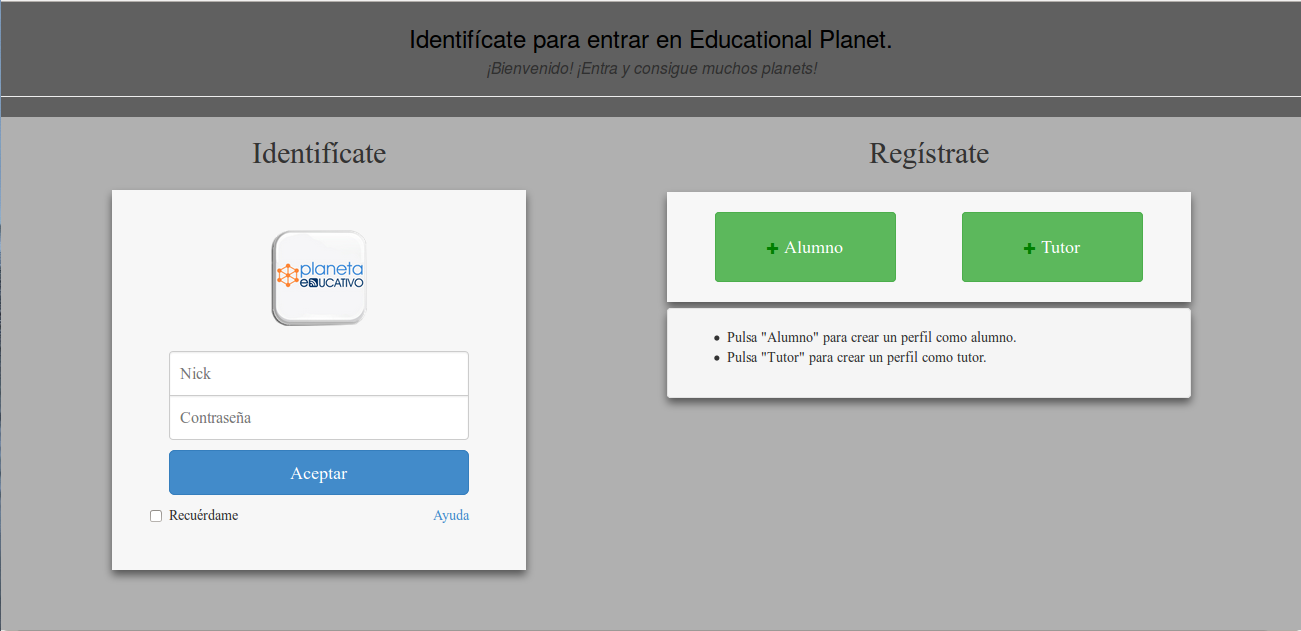
\includegraphics[width=17cm, keepaspectratio]{imagenes/PaginaInicio}}
  \caption{P\'agina de inicio.}
  \label{figura:inicio}
\end{figure}

\begin{itemize}
  \item {\bfseries Identif\'icate}: Iniciar sesi\'on con un formulario que aparece para introducir nombre de usuario y contrase\~na~\ref{figura:inicio1}(a).
  En caso de que los datos introducidos sean err\'oneos saldr\'a un mensaje indicando que se deben introducir datos v\'alidos~\ref{figura:inicio1}(b).
  \item {\bfseries Reg\'istrate}: Antes de iniciar sesi\'on como usuario dado de alta en la aplicaci\'on es obligatorio crearse un perfil pulsando sobre 
  uno de los dos botones que aparecen en verde. Con etiqueta ``Alumno'' para registrarse como alumno, y con etiqueta ``Tutor'' para registrarse como tutor.
\end{itemize} 

\begin{figure}[htbp] 
  \centering
  \subfigure[Formulario de inicio de sesi\'on.]{\Ovalbox{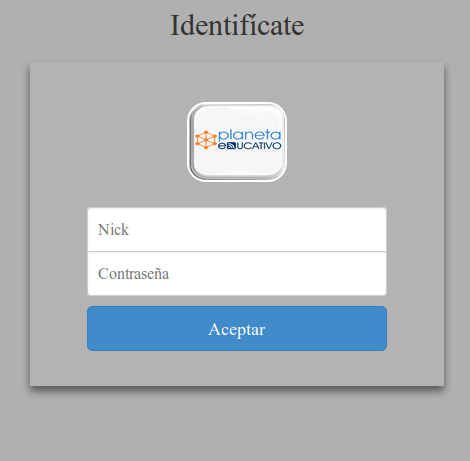
\includegraphics[width=7cm]{imagenes/InicioComoAlumno}}}
  \subfigure[Inicio de sesi\'on err\'onea.]{\Ovalbox{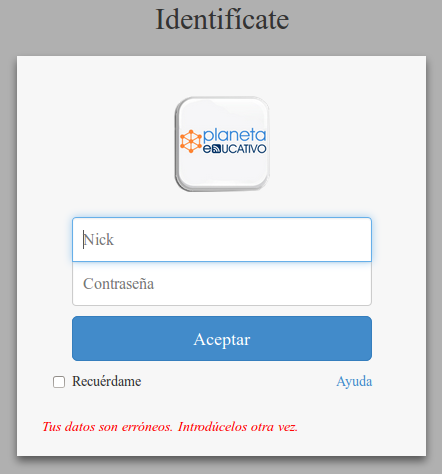
\includegraphics[width=7cm]{imagenes/InicioError}}}
  \caption{Inicio de sesi\'on.}
  \label{figura:inicio1}
\end{figure}



\section{P\'agina de registro}
La creaci\'on de un perfil de usuario pasa por rellenar los campos del formulario que se observan en ambas figuras. Tanto en el registro de  
alumnos~\ref{figura:registro}(a), como en el registro de tutores~\ref{figura:registro}(b) se rellenan los mismos campos: Una imagen, un nick de usuario,
un nombre y sus apellidos, un email y una contrase\~na.
\begin{figure}[htbp] 
  \centering
  \subfigure[Registro como alumno.]{\doublebox{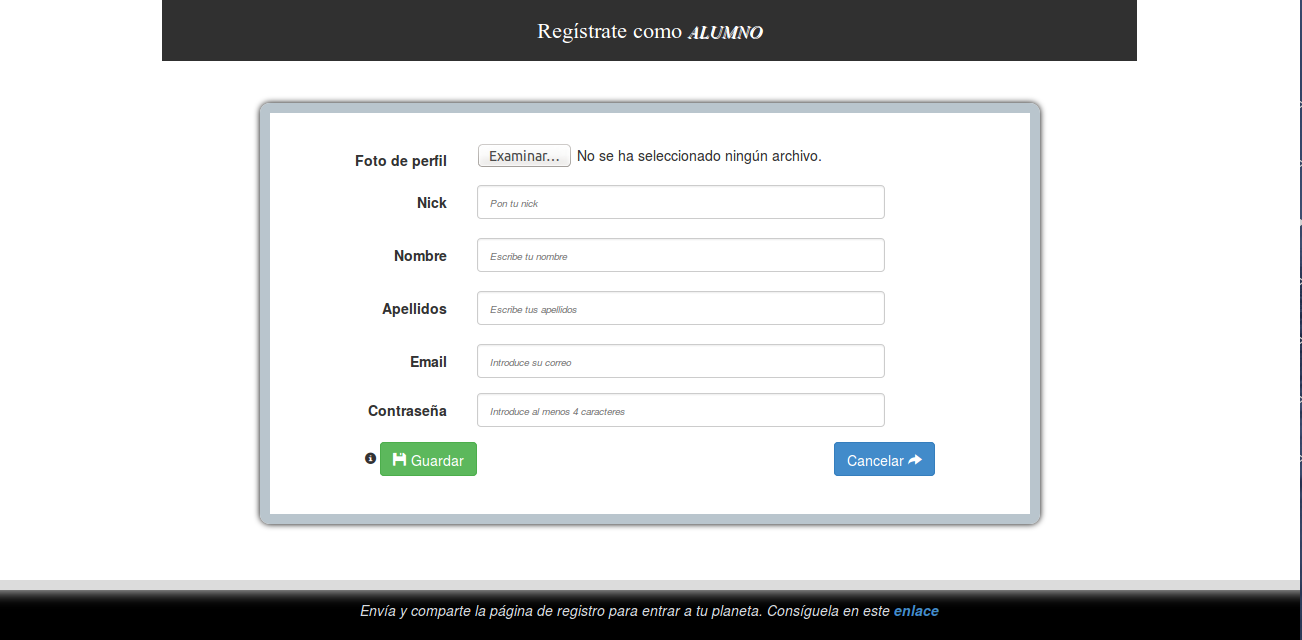
\includegraphics[width=12cm]{imagenes/RegistroAlumno}}}
  \subfigure[Registro como tutor.]{\doublebox{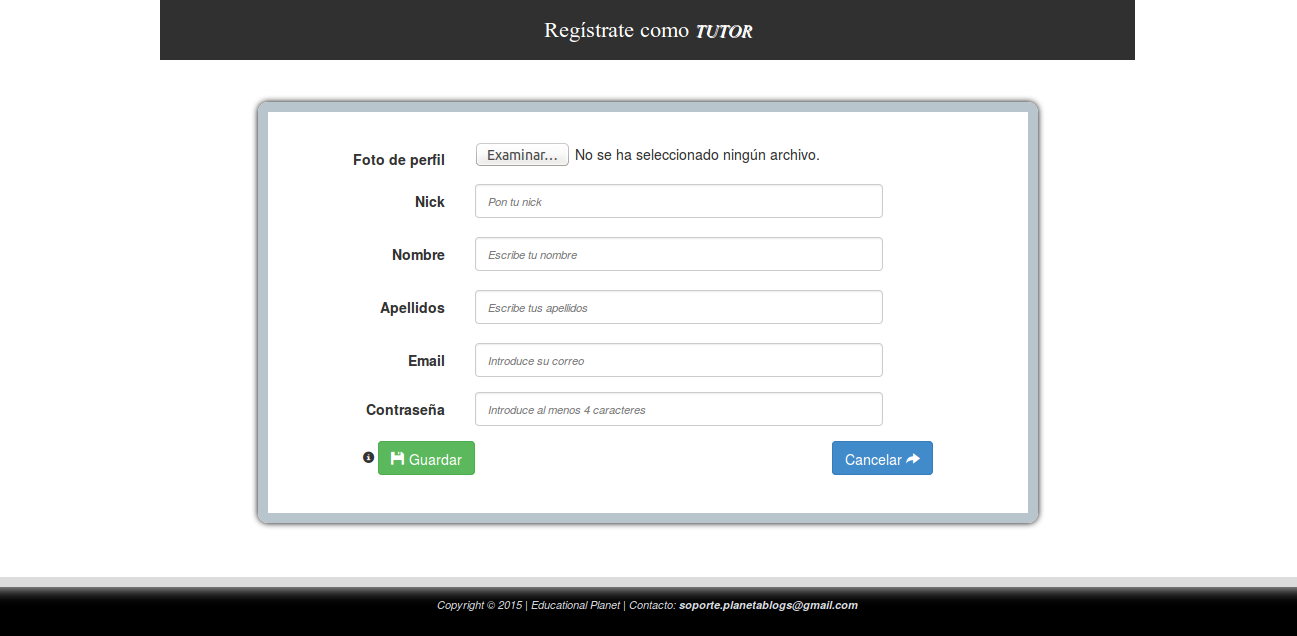
\includegraphics[width=12cm]{imagenes/RegistroTutor}}}
  \caption{Inicio de sesi\'on}
  \label{figura:registro}
\end{figure}

El nick de usuario debe ser \'unico y no estar ocupado por ning\'un integrante de la aplicaci\'on. Seg\'un se teclea el nick se mostrar\'a si el nick est\'a 
apropiado por otro usuario en rojo o por el contrario se encuentra libre en verde (figura~\ref{figura:registro1}).\\\\
\begin{figure}[htbp]
  \centering
  \Ovalbox{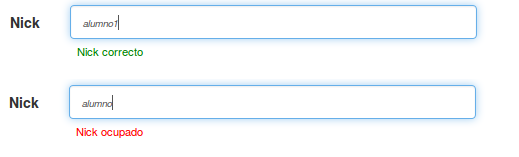
\includegraphics[width=17cm, keepaspectratio]{imagenes/NickCorrectoOcupado}}
  \caption{Rellenar nick}
  \label{figura:registro1}
\end{figure}

Una vez relleno todos los campos del formulario se debe pulsar el bot\'on ``Guardar''. Si los datos son correctos se redirigir\'a a la p\'agina de inicio
de sesi\'on para que se proceda con la identificaci\'on. Si los datos son incorrectos se mostrar\'a una alerta o panel rojo debajo del formulario con un 
mensaje de informaci\'on err\'onea que anime a introducirlos otra vez. Se puede dar al icono ``X'' para cerrar el panel 
(figura~\ref{figura:registro2}).
\begin{figure}[htbp] 
  \centering
  \Ovalbox{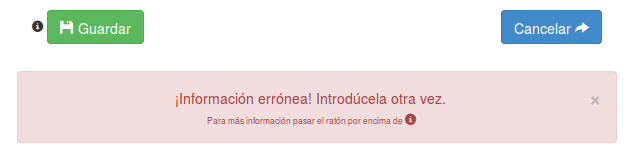
\includegraphics[width=17cm, keepaspectratio]{imagenes/RegistroAlumnoError}}
  \caption{Registro err\'oneo}
  \label{figura:registro2}
\end{figure}

Seg\'un se ve en el mensaje de informaci\'on err\'onea existe la posibilidad de pasar el rat\'on por encima del icono de informaci\'on, a la izquierda del 
bot\'on ``Guardar''. Al realizar esta acci\'on se abre una alerta azul con un mensaje recordatorio de como deben ser los datos introducidos para un correcto
registro de perfil de usuario. Son cinco condiciones que se enumeran en la figura~\ref{figura:registro3}.
\begin{figure}[htbp] 
  \centering
  \Ovalbox{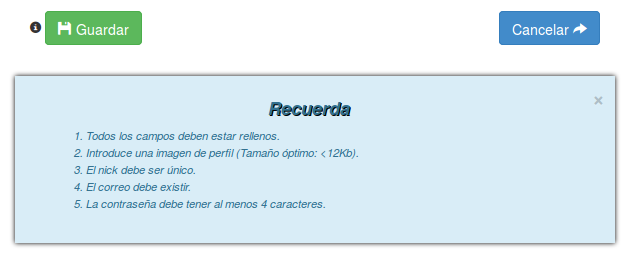
\includegraphics[width=17cm, keepaspectratio]{imagenes/RegistroAlumnoInfo}}
  \caption{Informaci\'on de registro}
  \label{figura:registro3}
\end{figure}

Otra acci\'on a destacar dentro de la p\'agina de registro es la opci\'on de cancelar el registro con el bot\'on azul ``Cancelar''. Si se pulsa sobre \'el se
redirigir\'a a la p\'agina de inicio de sesi\'on.


\section{Presentaci\'on de tutor}
\label{app:presentaciontutor}
Despu\'es de haber realizado el registro de usuario como tutor y de introducir nombre de usuario y contrase\~na en la p\'agina de inicio, la sesi\'on 
comienza con la presentaci\'on de tutor o perfil de tutor (figura~\ref{figura:tutor}). En la cabecera se ofrece la posibilidad de desconectar la sesi\'on (a la derecha, pulsando el 
enlace ``Desconectar'' en rojo). Aparece una pesta\~na ``Mis hilos'' la cual tiene la funci\'on de actualizar la p\'agina de perfil 
de tutor y tambi\'en otra pesta\~na ``Resetear contrase\~na'' la cual se encargar\'a de redirigir a una p\'agina formulario con la posibilidad de
modificar la contrase\~na de cualquier usuario. Adem\'as se exhibe una foto del usuario y un t\'itulo con la expresi\'on 
\textit{Espacio de NOMBRE APELLIDO1 APELLIDO2} indicando de quien es el perfil.

\begin{figure}[htbp] 
  \centering
  \doublebox{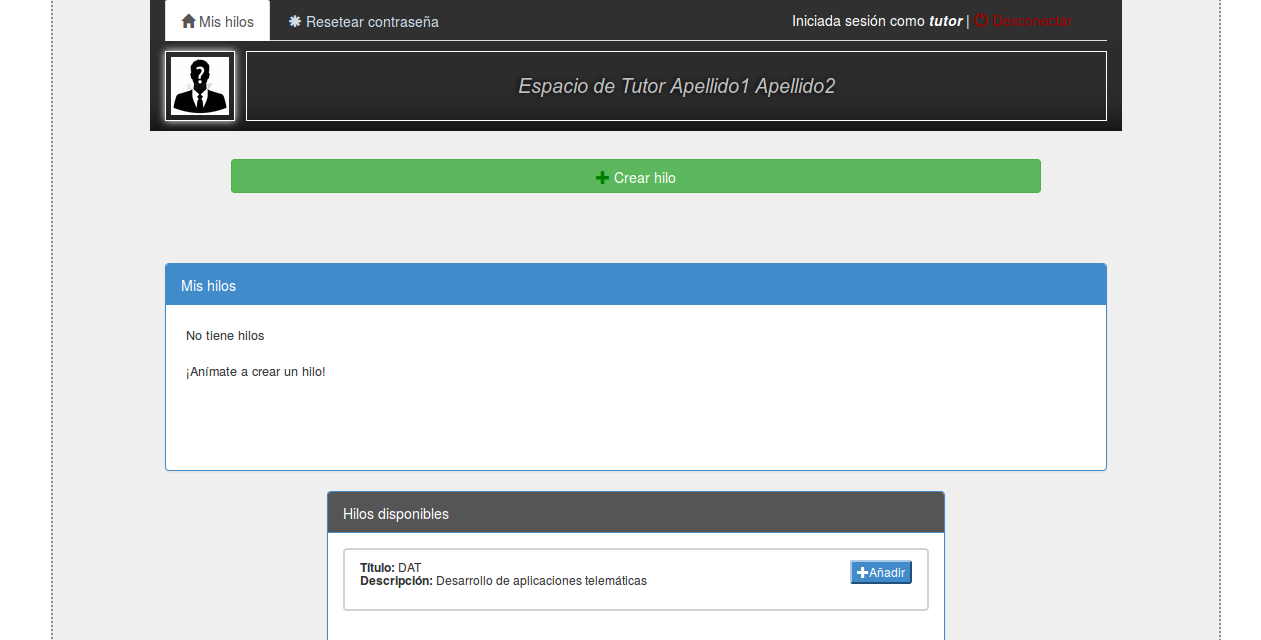
\includegraphics[width=17cm, keepaspectratio]{imagenes/PresentacionTutor}}
  \caption{P\'agina de presentaci\'on de tutor.}
  \label{figura:tutor}
\end{figure}

Las secciones que se incluyen en la presentaci\'on de un tutor son:

\begin{itemize}
  \item {\bfseries Crear hilo}: Al presionar el bot\'on verde y alargado ``Crear hilo'', se extiende un formulario como el de la figura~\ref{figura:tutor1} 
  por el cual un tutor puede fundar un hilo asignando un t\'itulo y una descripci\'on breve sobre la tem\'atica del hilo. Al enviar el formulario, el hilo 
  pasa directamente a la secci\'on de ``Hilos disponibles''.
  \begin{figure}[htbp] 
    \centering
    \Ovalbox{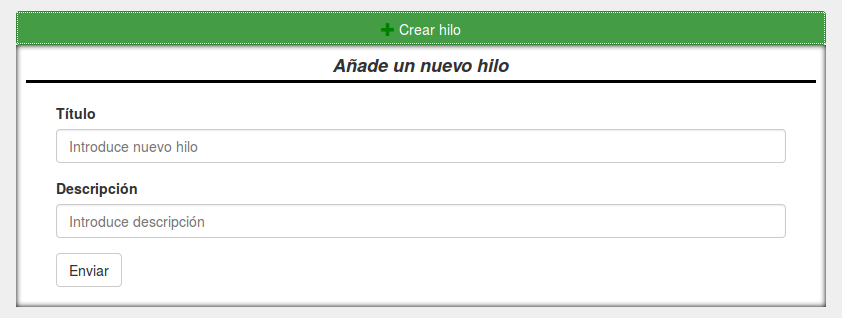
\includegraphics[width=17cm, keepaspectratio]{imagenes/PresentacionTutorCrearHilo}}
    \caption{Formulario para la creaci\'on de un hilo.}
    \label{figura:tutor1}
  \end{figure}
  
  \item {\bfseries Hilos disponibles}: Se presentan todos los hilos creados anteriormente a los que el tutor no est\'a suscrito (ya sean creados o no por 
  el tutor del propio perfil). Sin embargo, como se muestra en la figura~\ref{figura:tutor2}, al lado de cada hilo se expondr\'a un bot\'on ``A\~nadir'' 
  solamente si ha sido creado por dicho tutor. Si se presiona pasar\'a a la secci\'on de ``Mis hilos''.
  \begin{figure}[htbp] 
    \centering
    \Ovalbox{\includegraphics[width=17cm, keepaspectratio]{imagenes/PresentacionTutorHilosDisponibles}}
    \caption{Secci\'on de \textit{Hilos disponibles} en una presentaci\'on de tutor.}
    \label{figura:tutor2}
  \end{figure}
  
  \item {\bfseries Mis hilos}: Se presentan todos los hilos a los que el tutor est\'a suscrito (figura~\ref{figura:tutor3}). Para cada hilo se hallan las 
  alternativas de apretar el bot\'on ``Eliminar'' para suprimir el hilo de esta secci\'on y enviarlo a ``Hilos disponibles'', o de presionar el bot\'on
  ``Visitar'' para acceder a la p\'agina propia de la asignatura pertinente. Al pulsar sobre el bot\'on ``Eliminar'' se abre un cuadro de di\'alogo en el 
  centro de la pantalla para asegurarse de que es la acci\'on que realmente se quiere realizar.
  \begin{figure}[htbp] 
    \centering
    \Ovalbox{\includegraphics[width=17cm, keepaspectratio]{imagenes/PresentacionTutorMisHilos}}
    \caption{Secci\'on de \textit{Mis hilos} en una presentaci\'on.}
    \label{figura:tutor3}
  \end{figure}
\end{itemize} 


\section{Presentaci\'on de alumno}
\label{app:presentacionalumno}
Despu\'es de haber realizado el registro de usuario como alumno y de introducir nombre de usuario y contrase\~na en la p\'agina de inicio, la sesi\'on 
comienza con la presentaci\'on de alumno o perfil de alumno (figura~\ref{figura:alumno}). En la cabecera se ofrece la posibilidad de desconectar la sesi\'on 
(a la derecha, pulsando el enlace ``Desconectar'' en rojo). S\'olo aparece una pesta\~na ``Mis hilos'', a la izquierda, la cual tiene la funci\'on de 
actualizar la p\'agina de perfil de alumno. Tambi\'en se exhibe una foto del usuario y un t\'itulo con la expresi\'on 
\textit{Espacio de NOMBRE APELLIDO1 APELLIDO2} indicando de quien es el perfil.

\begin{figure}[htbp] 
  \centering
  \doublebox{\includegraphics[width=17cm, keepaspectratio]{imagenes/PresentacionAlumno}}
  \caption{P\'agina de presentaci\'on de alumno.}
  \label{figura:alumno}
\end{figure}

Las secciones que se incluyen en la presentaci\'on de un alumno son:

\begin{itemize}
  \item {\bfseries Hilos disponibles}: Se presentan todos los hilos creados anteriormente a los que el alumno no est\'a suscrito. Como se ve en la 
  figura~\ref{figura:alumno1} cada hilo expone un bot\'on ``Guardar y a\~nadir'' para que cuando sea presionado, el hilo correspondiente pase a la 
  secci\'on de ``Mis hilos''. Pero antes se debe haber introducido un enlace \textit{RSS} v\'alido en el formulario proporcionado para ello. En ese 
  \textit{RSS} (blog) ser\'a donde el alumno escribir\'a sus entradas para que se publiquen autom\'aticamente dentro de la aplicaci\'on, concretamente
  en el hilo al que pertenecen.
  \begin{figure}[htbp] 
    \centering
    \Ovalbox{\includegraphics[width=17cm, keepaspectratio]{imagenes/PresentacionAlumnoHilosDisponibles}}
    \caption{Secci\'on de \textit{Hilos disponibles} en una presentaci\'on de alumno.}
    \label{figura:alumno1}
  \end{figure}
  
  En caso de que el \textit{RSS} no sea v\'alido se recargar\'a la p\'agina de presentaci\'on de alumno indicando un error en un panel de alerta marr\'on 
  (figura~\ref{figura:alumno2}).
  \begin{figure}[htbp] 
    \centering
    \Ovalbox{\includegraphics[width=17cm, keepaspectratio]{imagenes/HiloAlumnoErrorRss}}
    \caption{Error al introducir \textit{RSS} en una presentaci\'on de alumno.}
    \label{figura:alumno2}
  \end{figure}
  
  \item {\bfseries Mis hilos}: Se presentan todos los hilos a los que el alumno est\'a suscrito (secci\'on id\'entica a la que expone la presentaci\'on de 
  tutor (figura~\ref{figura:tutor3}). Para cada hilo se hallan las alternativas de apretar el bot\'on ``Eliminar'' para suprimir el hilo de esta secci\'on y 
  enviarlo a ``Hilos disponibles'', o de presionar el bot\'on ``Visitar'' para acceder a la p\'agina propia de la asignatura pertinente. Al pulsar sobre el 
  bot\'on ``Eliminar'' se abre un cuadro de di\'alogo en el centro de la pantalla para asegurarse de que es la acci\'on que realmente se quiere realizar, 
  avisando de los riesgos que ello conlleva (figura~\ref{figura:alumno3}).
  \begin{figure}[htbp] 
    \centering
    \Ovalbox{\includegraphics[width=17cm, keepaspectratio]{imagenes/PresentacionAlumnoEliminarHilo}}
    \caption{Eliminar hilo de la secci\'on de \textit{Mis hilos} en una presentaci\'on de alumno.}
    \label{figura:alumno3}
  \end{figure}
\end{itemize} 


\section{Hilo de alumno}
\label{app:hiloalumno}
La p\'agina de una asignatura concreta por parte de un alumno se visualiza despu\'es de dar al bot\'on ``Visitar'' en su presentaci\'on. En la 
figura~\ref{figura:hiloalumno} se muestra un hilo vac\'io en sus inicios, sin entradas.
\begin{figure}[htbp] 
  \centering
  \doublebox{\includegraphics[width=17cm, keepaspectratio]{imagenes/HiloAlumno}}
  \caption{Hilo vac\'io de un alumno.}
  \label{figura:hiloalumno}
\end{figure}

Para ver tus propias entradas es necesario escribir previamente en el blog asociado a esa asignatura. En la aplicaci\'on se ejecuta un script 
autom\'atico cada sesenta segundos que se encarga de guardar y actualizar las entradas de todos los blogs de todos los alumnos que est\'en suscritos al 
hilo. Cada vez que un usuario suscrito escriba un mensaje en su blog, este mensaje se plasmar\'a en el contenedor de la p\'agina. Para recargar la p\'agina 
se puede pulsar sobre la pesta\~na que est\'a activa en cabecera, y que expone el t\'itulo del hilo.
\begin{figure}[htbp] 
  \centering
  \doublebox{\includegraphics[width=17cm, keepaspectratio]{imagenes/HiloAlumnoLleno}}
  \caption{Hilo con entradas de un alumno.}
  \label{figura:hiloalumno1}
\end{figure}

\subsection{Entradas}
El usuario puede interactuar con una entrada (\ref{figura:hiloalumno1}) de diversas maneras:
\begin{itemize}
  \item {\bfseries Valoraci\'on cuantitativa}: Los botones verde y rojo aportan una valoraci\'on cuantitativa. Si se decide por pulsar 
  la valoraci\'on positiva (bot\'on verde), el alumno que cre\'o la entrada recibir\'a una bonificaci\'on de dos \textit{planets} (el \textit{planet} es la 
  moneda de la aplicaci\'on). Si se decide por pulsar la valoraci\'on negativa (bot\'on rojo), el alumno que cre\'o la entrada recibir\'a una penalizaci\'on 
  de un \textit{planet}. Si un usuario presiona uno de los dos botones sobre una entrada, no podr\'a valorar m\'as veces en ella, ya que ambos botones 
  emerger\'an deshabilitados con su contador total. En este momento, el usuario podr\'a visualizar el total de valoraciones positivas y negativas que posee 
  esa entrada.
  \item {\bfseries Valoraci\'on cualitativa}: El \'area facilitado para escribir un comentario aporta una valoraci\'on cualitativa. Para mostrar dicho 
  \'area hay que desplegar el bot\'on ``Mostrar comentarios'', al lado del cual se encuentra un contador total de comentarios escritos sobre esa entrada.
  Si el usuario decide proponer una opini\'on, este usuario recibir\'a una bonificaci\'on de tres \textit{planets} al presionar el bot\'on ``Enviar'', y 
  simult\'aneamente se mostrar\'a un popup informando de que acabas de recibir tres \textit{planets} (ver figura~\ref{figura:hiloalumno6})
  \begin{figure}[htbp] 
    \centering
    \Ovalbox{\includegraphics[width=17cm, keepaspectratio]{imagenes/HiloAlumnoInfoComentario}}
    \caption{Informaci\'on emergente de un comentario.}
    \label{figura:hiloalumno6}
  \end{figure}
  
  Si ese comentario es eliminado, el usuario obtendr\'a una penalizaci\'on de tres \textit{planets}.
  
  \item {\bfseries Puntuaci\'on del tutor}: La valoraci\'on del tutor se muestra a la derecha de los botones verde y rojo. En caso de que el tutor haya
  calificado la entrada se podr\'a ver la puntuaci\'on dada en naranja (\ref{figura:hiloalumno7}(a)). En caso contrario, se obtendr\'a una calificaci\'on de 
  ``Sin Calificar'' en azul (\ref{figura:hiloalumno7}(b)).
  \begin{figure}
    \centering
    \subfigure[Entrada valorada por el tutor.]{\Ovalbox{\includegraphics[width=11cm]{imagenes/ValoracionTutorCalificada}}}
    \subfigure[Entrada no valorada por el tutor.]{\Ovalbox{\includegraphics[width=11cm]{imagenes/ValoracionTutorNoCalificada}}}
    \caption{\textit{Valoraciones del tutor en entradas.}}
    \label{figura:hiloalumno7}
  \end{figure}
  
  \item {\bfseries Ojear blog}: En una entrada existen dos enlaces que redirigir\'an directamente al blog del alumno donde se ubican todas sus entradas 
  fuera de la aplicaci\'on. Los dos enlaces aparecen en forma de ``Nombre y apellidos'' y ``Nick'' (al lado de la fecha, en negrita).
  
  Si se presiona sobre el enlace del t\'itulo, se abrir\'a otra pesta\~na con la ubicaci\'on de la propia entrada dentro del blog.
  \item {\bfseries Visualizar informaci\'on del usuario}: Al pasar el rat\'on por encima del enlace ``Nombre y apellidos'' brotar\'a un mensaje informativo 
  con datos del usuario: Foto de perfil, nombre, apellidos, puntuaci\'on total y nivel (\ref{figura:hiloalumno2}).
  \begin{figure}[htbp] 
    \centering
    \Ovalbox{\includegraphics[width=17cm, keepaspectratio]{imagenes/HiloAlumnoInfoAlumno}}
    \caption{Informaci\'on emergente de un alumno.}
    \label{figura:hiloalumno2}
  \end{figure}
  
  \item {\bfseries Informaci\'on adicional}: Adem\'as, la entrada muestra el n\'umero de identificaci\'on seguido de ``\#'' y una foto. Para cada hilo no puede existir
  dos entradas con un mismo n\'umero identificativo.
\end{itemize}

\subsection{Logo}
Debajo de la cabecera, en la parte izquierda se puede observar el logo y el nombre de la aplicaci\'on, junto con una frase motivadora que hace de eslogan.
Cada vez que se recarga la p\'agina o se presiona sobre la frase, \'esta se modifica autom\'atica y aleatoriamente de entre un conjunto de 21 oraciones 
(~\ref{figura:logonombrefrase})
\begin{figure}[htbp] 
  \centering
  \Ovalbox{\includegraphics[width=17cm, keepaspectratio]{imagenes/LogoNombreFrase}}
  \caption{Logo, nombre y eslogan aleatorio de la aplicaci\'on.}
  \label{figura:logonombrefrase}
\end{figure}

\subsection{Entradas m\'as valoradas}
Otra parte importante se sit\'ua en la parte superior de la p\'agina debajo de la cabecera, donde se agrupan las entradas con m\'as valoraci\'on 
cuantitativa de la asignatura. Se aplica una f\'ormula, la cual suma dos \textit{planets} por cada valoraci\'on positiva y resta un \textit{planet} por 
cada valoraci\'on negativa. Se calcula el total de la suma y se plasman las diez mejores entradas.

En la figura~\ref{figura:hiloalumno3} se muestra la secci\'on donde encajan las diez entradas seleccionadas. Cada una se rellena con el n\'umero de 
posici\'on que ocupa, su identificador, su t\'itulo, la persona que lo escribi\'o, su fecha, las valoraciones positivas y negativas (en color verde y rojo,
respectivamente), y por \'ultimo su n\'umero total de \textit{planets}. Son enlaces que al pinchar encima de cada entrada te lleva a la p\'agina del post 
correspondiente.
\begin{figure}[htbp] 
  \centering
  \Ovalbox{\includegraphics[width=17cm, keepaspectratio]{imagenes/HiloAlumnoEntradasValoradas}}
  \caption{Entradas m\'as valoradas del hilo de alumno.}
  \label{figura:hiloalumno3}
\end{figure}

\subsection{Usuarios suscritos}
En la columna situada a la derecha se re\'unen en una tabla todos los alumnos suscritos en el hilo. Esta tabla se compone de tres columnas correspondientes
al nick de usuario, nombre y apellidos de usuario, y un enlace que redirecciona al RSS del blog del alumno. 
(~\ref{figura:hiloalumno4}).
\begin{figure}[htbp] 
  \centering
  \Ovalbox{\includegraphics[width=17cm, keepaspectratio]{imagenes/HiloAlumnoUsuariosSuscritos}}
  \caption{Usuarios suscritos al hilo.}
  \label{figura:hiloalumno4}
\end{figure}

\subsection{Paginador y flecha}
Estas dos funciones se pueden ver en la figura~\ref{figura:hiloalumno5}.

El paginador se encuentra en la parte inferior de la p\'agina. Cada p\'agina del hilo mostrar\'a las cinco entradas m\'as recientes, las posteriores cinco 
las pondr\'a en la siguiente p\'agina y as\'i sucesivamente.

Otra funci\'on a\~nadida es la flecha de subida situada en la parte inferior derecha de la pantalla. \'Esta aparece cuando desciende el scroll una 
determinada altura. Si se pulsa sobre ella, el scroll asciende autom\'aticamente hasta la parte superior de la p\'agina.
\begin{figure}[htbp] 
  \centering
  \Ovalbox{\includegraphics[width=17cm, keepaspectratio]{imagenes/HiloAlumnoPaginatorYFlecha}}
  \caption{Paginador y flecha.}
  \label{figura:hiloalumno5}
\end{figure}

\section{Hilo de profesor}
Se conservan las mismas funciones que en la secci\'on~\ref{app:hiloalumno} (hilo de alumno) con algunos cambios en ``Entradas'' y en ``Usuarios 
suscritos''. En la figura~\ref{figura:hiloprofesor} se observa como estos cambios se reducen simplemente a que un tutor tiene el permiso de eliminar 
cualquier entrada, eliminar cualquier alumno de un determinado hilo y valorar cualquier entrada de forma cuantitativa.
\begin{figure}[htbp] 
  \centering
  \Ovalbox{\includegraphics[width=17cm, keepaspectratio]{imagenes/HiloTutorEntradas}}
  \caption{Hilo con entradas de un tutor.}
  \label{figura:hiloprofesor}
\end{figure}

Al pulsar el bot\'on ``Eliminar entrada'' se abrir\'a una alerta de aviso con unos puntos que se podr\'an leer para confirmar si realmente se quiere esa 
eliminaci\'on o no. Ver figura~\ref{figura:hiloprofesor1}(a).

Al pulsar el bot\'on ``Eliminar'' se abrir\'a otra alerta de aviso con unos puntos que se podr\'an leer para confirmar si realmente se quiere eliminar ese
usuario de ese hilo o no. Ver figura~\ref{figura:hiloprofesor1}(b).
\begin{figure}
  \centering
  \subfigure[Eliminar entrada.]{\Ovalbox{\includegraphics[width=11cm]{imagenes/HiloTutorEliminarEntrada}}}
  \subfigure[Eliminar alumno.]{\Ovalbox{\includegraphics[width=11cm]{imagenes/HiloTutorEliminarAlumno}}}
  \caption{\textit{Eliminaciones en hilo de tutor.}}
  \label{figura:hiloprofesor1}
\end{figure}

La valoraci\'on del tutor se realiza a trav\'es de la parte de la entrada vista en la figura~\ref{figura:hiloprofesor2}. Los posibles valores est\'an dentro
de un rango con un l\'imite m\'aximo que es superior al valor de un ``UP'' y con un l\'imite m\'inimo que es inferior al valor de un ``DOWN''. El intervalo de
\textit{planets} es [-2, -1, 1, 2, 3, 4]. Una vez seleccionado el valor, se env\'ia al pulsar sobre el bot\'on ``Enviar'' azul.
\begin{figure}[htbp] 
  \centering
  \Ovalbox{\includegraphics[width=17cm, keepaspectratio]{imagenes/HiloTutorValoracionEntradas}}
  \caption{Valoraci\'on de tutor en una determinada entrada.}
  \label{figura:hiloprofesor2}
\end{figure}

\section{Opciones de men\'u en cabecera}
Dentro de la cabecera del hilo de un alumno o de un tutor se encuentran varias opciones. Cada pesta\~na esconde un enlace que redirigir\'a a su 
correspondiente p\'agina. Una vez el usuario se encuentre en la p\'agina del enlace pulsado, la pesta\~na se mostrar\'a activa en color blanco mientras que 
las dem\'as pesta\~nas permanecer\'an inactivas en color negro.

\subsection{Mis hilos}
La pesta\~na de ``Mis hilos'' devolver\'a al usuario a su perfil o presentaci\'on descrita anteriormente en la secci\'on~\ref{app:presentacionalumno} (si el usuario
es un alumno) o en la secci\'on~\ref{app:presentaciontutor} (si el usuario es un tutor).

\subsection{T\'itulo del hilo}
Esta opci\'on es la p\'agina principal de cada hilo. Hay que tener en cuenta que por debajo de la aplicaci\'on se ejecuta un script autom\'aticamente cada 
sesenta segundos para actualizar y guardar entradas nuevas de los distintos blogs, por lo que si se pulsa sobre esta pesta\~na, \'esta har\'a la funci\'on 
de recargar la p\'agina para plasmar esas actualizaciones peri\'odicas en el contenedor de entradas.

\subsection{Buscar}
La p\'agina asociada a la pesta\~na ``Buscar'' se muestra en la figura~\ref{fig:buscar} mostrada en la secci\'on~\ref{sec:buscar} que explica la 
vista ``B\'usqueda avanzada''.

La b\'usqueda se puede realizar por identificador de entrada o por nick de usuario. Al elegir una opci\'on, se debe escribir un identificador de entrada o 
un nick de usuario v\'alidos. En caso de \'exito se visualizar\'a la entrada por introducci\'on del identificador o las entradas por introducci\'on del nick
(figura~\ref{fig:buscarajax}). En caso de no introducir un texto v\'alido se notificar\'a con un mensaje en rojo en el contenedor.

\subsection{Puntuaci\'on}
Si se despliega el men\'u ``Puntuaci\'on'' emergen dos opciones:
\begin{itemize}
  \item {\bfseries Ranking}: La figura~\ref{fig:ranking} de la secci\'on~\ref{sec:ranking} muestra la p\'agina al pulsar sobre el enlace de la pesta\~na 
  ``Ranking''. La p\'agina es informativa en su mayor\'ia. Muestra el ranking del hilo en una tabla con cuatro columnas: Posici\'on, nick de usuario con su
  foto, puntuaci\'on total y nivel.
  
  El usuario puede interactuar con esta p\'agina poniendo el rat\'on encima de la foto para ampliarla, y encima del nivel para visualizar el color al que 
  est\'a asociado (\ref{figura:ranking}).
  \begin{figure}
    \centering
    \subfigure[Color asociado al nivel.]{\Ovalbox{\includegraphics[width=11cm]{imagenes/HiloAlumnoRankingColor}}}
    \subfigure[Foto de perfil ampliada.]{\Ovalbox{\includegraphics[width=11cm]{imagenes/HiloAlumnoRankingFoto}}}
    \caption{\textit{Interacciones de usuario en la p\'agina de Ranking.}}
    \label{figura:ranking}
  \end{figure}
  \item {\bfseries Estad\'isticas}: La figura~\ref{fig:estadisticas} de la secci\'on~\ref{sec:estadisticas} muestra la p\'agina al pulsar sobre el enlace de la pesta\~na 
  ``Estad\'isticas''. La p\'agina es informativa. Da la opci\'on al usuario de elegir las estad\'isticas que quiere visualizar (\ref{figura:estadisticas}).
  
  \begin{figure}
    \centering
    \Ovalbox{\includegraphics[width=17cm, keepaspectratio]{imagenes/HiloAlumnoEstadisticasRB}}
    \caption{Opciones de estad\'isticas.}
    \label{figura:estadisticas}
  \end{figure}
  Cada pesta\~na del acorde\'on refleja la informaci\'on de un usuario. La informaci\'on que se visualice depende de las opciones que el usuario haya elegido.
  En la figura~\ref{figura:estadisticas1} se puede observar las tres opciones posibles: S\'olo estad\'isticas generales (a), s\'olo resumen de entradas (b) o 
  ambas (c).
  \begin{figure}
  \centering
  \subfigure[Estad\'isticas generales.]{\Ovalbox{\includegraphics[width=11cm]{imagenes/HiloAlumnoEstadisticasGenerales}}}
  \subfigure[Resumen de entradas.]{\Ovalbox{\includegraphics[width=11cm]{imagenes/HiloAlumnoEstadisticasEntradas}}}
  \subfigure[Ambas opciones anteriores.]{\Ovalbox{\includegraphics[width=11cm]{imagenes/HiloAlumnoEstadisticasAmbas}}}
  \caption{\textit{Visualizaci\'on de opciones estad\'isticas.}}
  \label{figura:estadisticas1}
\end{figure}

  \item {\bfseries Informaci\'on}: La figura~\ref{fig:informacionpuntuaciones} de la secci\'on~\ref{sec:informacionpuntuaciones} muestra la p\'agina al 
  presionar el enlace de la pesta\~na ``Informaci\'on''. La p\'agina es plenamente informativa. Crea unas bases de juego muy importantes para que el usuario
  tenga noci\'on del sistema de puntuaciones. Tambi\'en se muestra una tabla con el rango de puntuaciones que pertenece a cada nivel. Si se pasa el rat\'on
  por encima del nivel, \'este se iluminar\'a con su color asociado. El nivel 0 es el rojo y el nivel m\'aximo es el verde.
\end{itemize}


\subsection{Ayuda}
La pesta\~na ``Ayuda'' muestra una serie de informaci\'on y consejos de uso meramente informativos sobre la aplicaci\'on. Adem\'as, se aconseja enviar a un 
correo electr\'onico espec\'ifico con sugerencias para futuras mejoras o con planteamientos de diversos problemas que se encuentren los usuarios 
(figura~\ref{figura:ayuda}).
\begin{figure}[htbp] 
  \centering
  \doublebox{\includegraphics[width=17cm, keepaspectratio]{imagenes/Ayuda}}
  \caption{Ayuda.}
  \label{figura:ayuda}
\end{figure}


\subsection{Cierre de sesi\'on}
El enlace en rojo ``Desconectar'' expuesto en la parte derecha de la cabecera se usa para cerrar la sesi\'on de usuario. Al presionarlo se saldr\'a de la 
aplicaci\'on y volver\'a a la p\'agina de inicio para logarse otra vez si se desea.\\
Si el usuario superpone el rat\'on encima del icono azul (a la derecha del enlace de desconectar), se despliega un popup con informaci\'on del creador del 
hilo (nombre y apellidos, y correo ~\ref{figura:infocreador})
\begin{figure}[htbp] 
  \centering
  \Ovalbox{\includegraphics[width=17cm, keepaspectratio]{imagenes/HiloAlumnoInfoCreador}}
  \caption{Informaci\'on del creador del hilo.}
  \label{figura:infocreador}
\end{figure}

%%%%%%%%%%%%%%%%%%%%%%%%%%%%%%%%%%%%%%%%%%%%%%%%%%%%%%%%%%%%%%%%%%%%%%%%%%%%%%%%
%%%%%%%%%%%%%%%%%%%%%%%%%%%%%%%%%%%%%%%%%%%%%%%%%%%%%%%%%%%%%%%%%%%%%%%%%%%%%%%%
% BIBLIOGRAFIA %
%%%%%%%%%%%%%%%%%%%%%%%%%%%%%%%%%%%%%%%%%%%%%%%%%%%%%%%%%%%%%%%%%%%%%%%%%%%%%%%%

\cleardoublepage

% Las siguientes dos instrucciones es todo lo que necesitas
% para incluir las citas en la memoria
\bibliographystyle{abbrv}
\bibliography{memoria}  % memoria.bib es el nombre del fichero que contiene
% las referencias bibliogrficas. Abre ese fichero y mira el formato que tiene,
% que se conoce como BibTeX. Hay muchos sitios que exportan referencias en
% formato BibTeX. Prueba a buscar en http://scholar.google.com por referencias
% y vers que lo puedes hacer de manera sencilla.
% Ms informacin: 
% http://texblog.org/2014/04/22/using-google-scholar-to-download-bibtex-citations/

\end{document}
